% !TeX document-id = {723fde2e-8374-4acb-a15d-4655fdd0b330}
% !TeX TXS-program:compile = txs:///pdflatex/[--shell-escape]
\pdfminorversion=7
%\RequirePackage[l2tabu, orthodox]{nag}
\documentclass[12pt,a4paper,twoside]{report}%report
%\usepackage[style=numeric, backend=bibtex]{biblatex}
\usepackage[style=numeric, backend=bibtex]{biblatex}
\addbibresource{cap/references.bib}
\usepackage{graphicx}
\usepackage[font=small,labelfont=bf]{caption}
\usepackage{hyperref}
\usepackage{subcaption}
%%%%%%
\usepackage[a4paper,width=150mm,top=25mm,bottom=25mm,bindingoffset=6mm]{geometry}
\usepackage[utf8]{inputenc}

%%fonts
%\usepackage{lmodern}
%\usepackage[qtm]{tgtermes}

\usepackage{xcolor}

%% code part
\usepackage{listings}
\usepackage{minted}
\usemintedstyle{bw}

%% TOREMOVE
\usepackage{easyReview}

%% ~
\usepackage{textcomp}
\newcommand{\mytexttilde}{\raisebox{0.5ex}{\texttildelow}}
%% error copy _
\usepackage[T1]{fontenc}
%\usepackage{lmodern}


%% pdf-A
%\usepackage[a-1b,mathxmp]{pdfx}[2018/12/22]
%\usepackage{colorprofiles}
%\usepackage{pdfa}

%\begin{filecontents*}[overwrite]{\jobname.xmpdata}
%	\Title{An implementation of Open-RMF in an industrial environment}
%	\Author{Michele Belletti}
%	\Language{en-GB}
%	\Subject{The abstract or short description.}
%	\Keywords{keyword1\sep keyword2\sep keyword3}
%\end{filecontents*}

\title{An implementation of Open-RMF in an industrial environment}
\author{Michele Belletti}
%\date{2025\\ December}

%\usepackage{blindtext}
%\usepackage{emptypage}
%\usepackage{graphicx}
%\usepackage{float}
%\usepackage{amsmath}
%\usepackage{gensymb}
%\usepackage{textcomp}
%\usepackage{booktabs}

%\usepackage{setspace}
%\setstretch{1.5}

%\usepackage{subcaption}

%\usepackage{multirow}

%\usepackage{natbib}
% modification to natbib citations
%\bibliographystyle{tmlr}
%\setcitestyle{authoryear,round,citesep={;},aysep={,},yysep={;}}

%\usepackage[format=hang,font=small,labelfont=bf]{caption}

%\usepackage{etoolbox}
%\renewcommand{\topfraction}{0.9}	% max fraction of floats at top
%\renewcommand{\bottomfraction}{0.8}	% max fraction of floats at bottom

%\setcounter{topnumber}{2}
%\setcounter{bottomnumber}{2}
%\setcounter{totalnumber}{4}     % 2 may work better
%\setcounter{dbltopnumber}{2}    % for 2-column pages
%\renewcommand{\dbltopfraction}{0.9}	% fit big float above 2-col. text
%\renewcommand{\textfraction}{0.07}	% allow minimal text w. figs

\begin{document}

\begin{figure}[h]
	\centering
	
\includegraphics[width=0.3\linewidth]{img/units_simbl.png}
\end{figure}
\hrule
\vspace*{10mm}
\begin{center}
{\large 	Dipartimento di Ingegneria e Architettura\\
	\vspace*{7mm}
	CORSO DI LAUREA IN INGEGNERIA DELL'ENERGIA\\ ELETTRICA E DEI SISTEMI\\
	\vspace*{7mm}
	PROVA FINALE\\}
\vspace{10mm}
{\huge AN IMPLEMENTATION OF\vspace{5mm}
OPEN-RMF IN AN\vspace{5mm}
INDUSTRIAL ENVIRONMENT}
\end{center}
\vspace{30mm}
Laureando: Michele Belletti
\mbox{}\hfill Relatore: \hspace{7.5mm} Stefano Seriani\\
\mbox{}\hfill Correlatori: \hspace{4mm} Roberto Pugliese\\
\mbox{}\hfill Georgios Kourousias\\
\vspace{30mm}

\begin{center}
	ANNO ACCADEMICO 2024-2025
\end{center}

%\maketitle
\tableofcontents

\part{Introduction}
This work presents a study on the new system, OPEN-RMF, which is still under active development but has reached a mature enough state to be deployed in mobile robots at Elettra Sincrotrone Trieste.
\chapter{Background and motivation}
Elettra Sincontrone Trieste\footnote{\href{https://www.elettra.eu/}{https://www.elettra.eu/}} is a major research facility that primarily provides users access to two light sources: the synchrotron Elettra and the free electron laser FERMI.
In addition to operating these sources, the facility actively researches new technologies and techniques to enhance its capabilities and operations. Many recent advancements are based on robotics, which, especially after the COVID-19 pandemic and with the rapid rise of large language models (LLMs), have enabled new ways for users to interact with the infrastructure, including robot-assisted information retrieval and package delivery services.
Previously, the facility developed a global planner, D-Star (D-star based optimized trajectory planner)\cite{10.1007/978-3-031-45770-8_29}, within the ROS 1 framework to enable robot navigation across large-scale environments.  However, as ROS 1 has reached end-of-life, the codebase must now be migrated to ROS 2.
Additionally, the facility employs robots from multiple vendors, each specialized in different tasks and not designed to coordinate with one another.
An environment that has narrow passages and lifts can create significant coordination challenges during navigation.
To address this issue,  Open-RMF\footnote{\href{https://www.open-rmf.org/}{https://www.open-rmf.org/}} has been developed in recent years as a multiplatform system for controlling and managing heterogeneous fleets of robots.
\chapter{Research questions and objectives}
The objectives of this thesis are: to integrate a Rover Mini robot from the company RoverRobotics \footnote{\href{https://roverrobotics.com/}{https://roverrobotics.com/}}
into the ROS 2 Nav2 ecosystem,\\
\begin{figure}[h]
	\centering
	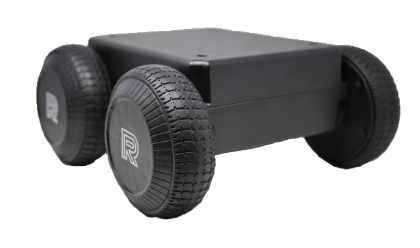
\includegraphics[width=0.4\linewidth]{img/RoverRoboticsMini.png}
	\captionof{figure}{RoverRobotics Rover Mini}
	\label{fig:RoverRobotics Rover Mini}
\end{figure}\\
to port the D-Star global planner from ROS 1 to ROS 2,
upgrade our Jobot rover from ROS 1 to ROS 2,\\
\begin{figure}[h]
	\centering
	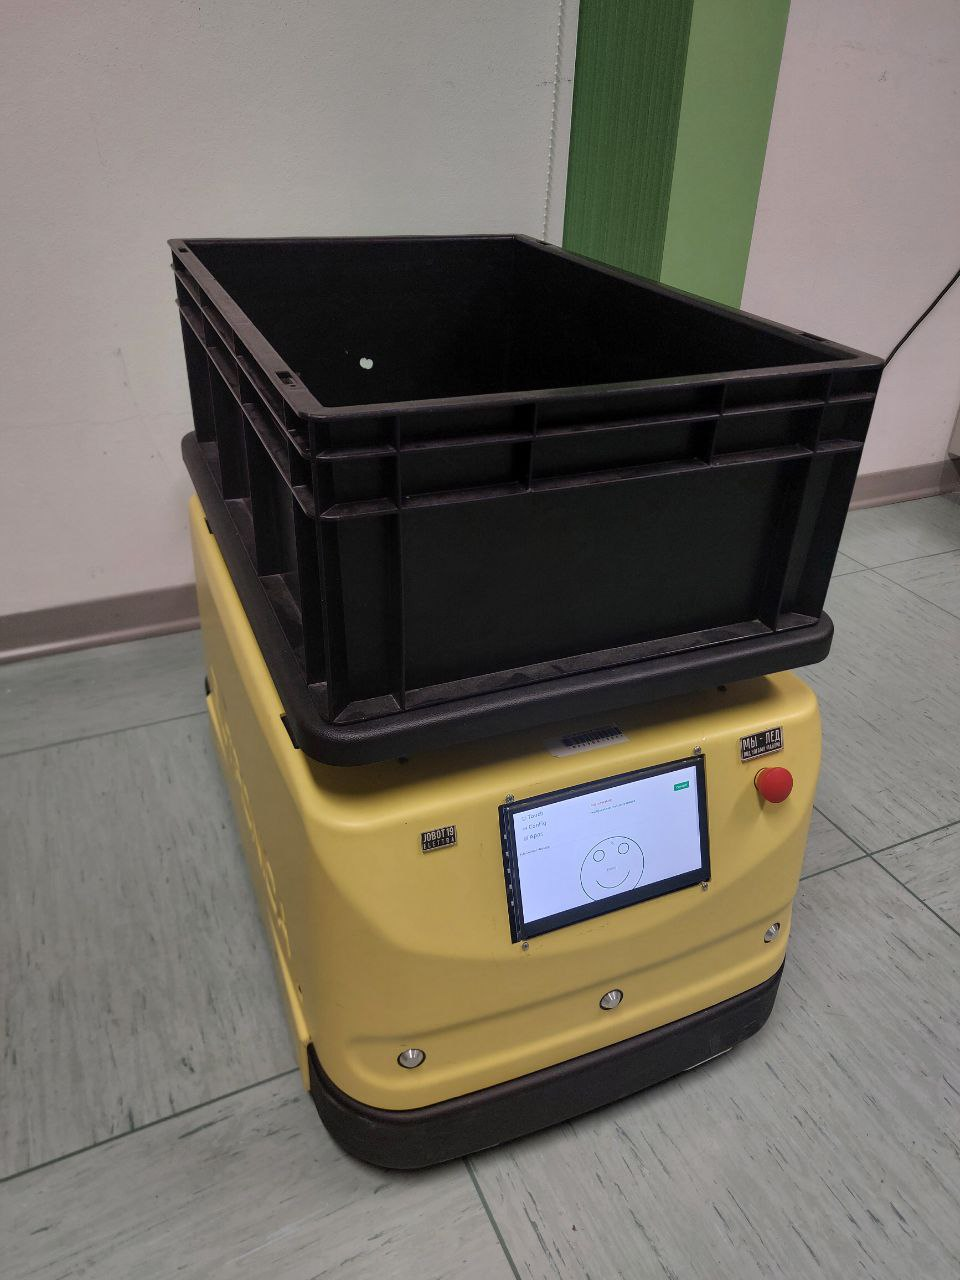
\includegraphics[width=0.3\linewidth]{img/jobot_robot.jpg}
	\captionof{figure}{Jobot Rover}
	\label{fig:Jobot Rover}
\end{figure}\\
incorporate the robot into the Open-RMF framework for centralized fleet management and evaluate the suitability of the Open-RMF ecosystem for deployment at the Elettra Sincrotrone Trieste.
\chapter{Scope and limitations}
The principal limitation is the current lack of access to lift control systems, which prevents direct integration and operation by the robot fleet. Additionally, there is no automated system for opening and closing doors. While Open-RMF offers a high degree of customizability, and human-in-the-loop interactions can be configured—such as triggering a light or sending a notification when a robot approaches a door—this method requires a human to manually open the door or operate the lift. However, such an approach is not ideal for achieving full autonomy.

\part{Literature Review}
In this section, we provide a description of the key technologies used in this thesis. We begin by describing the Robot Operating System (ROS) and its functionality, followed by an overview of the navigation system employed, and a discussion of how the Open-RMF fleet management system operates.
\chapter{Overview of ROS1 and ROS2}
The Robotics Operating System (ROS)\footnote{\href{https://www.ros.org/}{https://www.ros.org/}} is an open-source collection of tools and libraries designed to support the development of robotics applications. Despite its name, ROS is not an operating system (OS) in the traditional sense, but rather a software development kit (SDK) that provides developers with a comprehensive set of tools for building robotic systems. It offers several features typically associated with an OS, including hardware abstraction, low-level device control, implementation of commonly used functionalities, inter-process communication, and package management.
The ROS ecosystem is built upon the following core components:
\begin{itemize}
	\item \textbf{Middleware communication layer (RMW)}: Built on the Data Distribution Service (DDS) standard, this layer enables nodes to exchange information using an anonymous publish/subscribe pattern. This design promotes fault isolation, separation of concerns, and modular interfaces. ROS also supports synchronous, Remote Procedure Call (RPC)-style communication between services.\\While the default DDS implementation is eProsima Fast DDS  (\texttt{rmw\_fastrtps\_cpp}), this work uses Eclipse Cyclone DDS (\texttt{rmw\_cyclonedds\_cpp}) due to its better compatibility with the Nav2 navigation stack in ROS Humble.
	\item \textbf{Development tools}: ROS provides a suite of tools for managing and enhancing software development, including utilities for launching, introspection, debugging, visualization, plotting, logging, and playback.
	\item \textbf{Multi-machine support} ROS includes tools and libraries for retrieving, building, writing, and executing code across multiple computers and OS.
	\item \textbf{Community and governance}: ROS is supported by an active and extensive global community, coordinated primarily by Open Robotics\footnote{\href{https://www.openrobotics.org/}{https://www.openrobotics.org/}}, which serves as the central organization for its development and maintenance.
\end{itemize}
\newpage
\section{Structure of ROS}
The official ROS documentation\footnote{\href{https://docs.ros.org/en/rolling/index.html}{https://docs.ros.org/en/rolling/index.html}} provides comprehensive information about the system.  All communication in ROS is handled through the \textbf{ROS Graph} , a peer-to-peer network of processes (called nodes) that execute concurrently and exchange information with one another. Some components of this graph are described below. Note that some of the functionalities described are specific to ROS 2 and are not available in ROS 1:
\begin{itemize}
	\item \textbf{Nodes}: A node is a modular process that performs a specific task. Nodes communicate with each other through topics, services, actions, and parameters. In ROS 2, nodes can be implemented as \textbf{LifecycleNode}\label{LifecycleNode}, which provide a managed state machine with defined transitions for startup and shutdown, enabling more deterministic behavior.
	\begin{figure}[h]
	\centering
	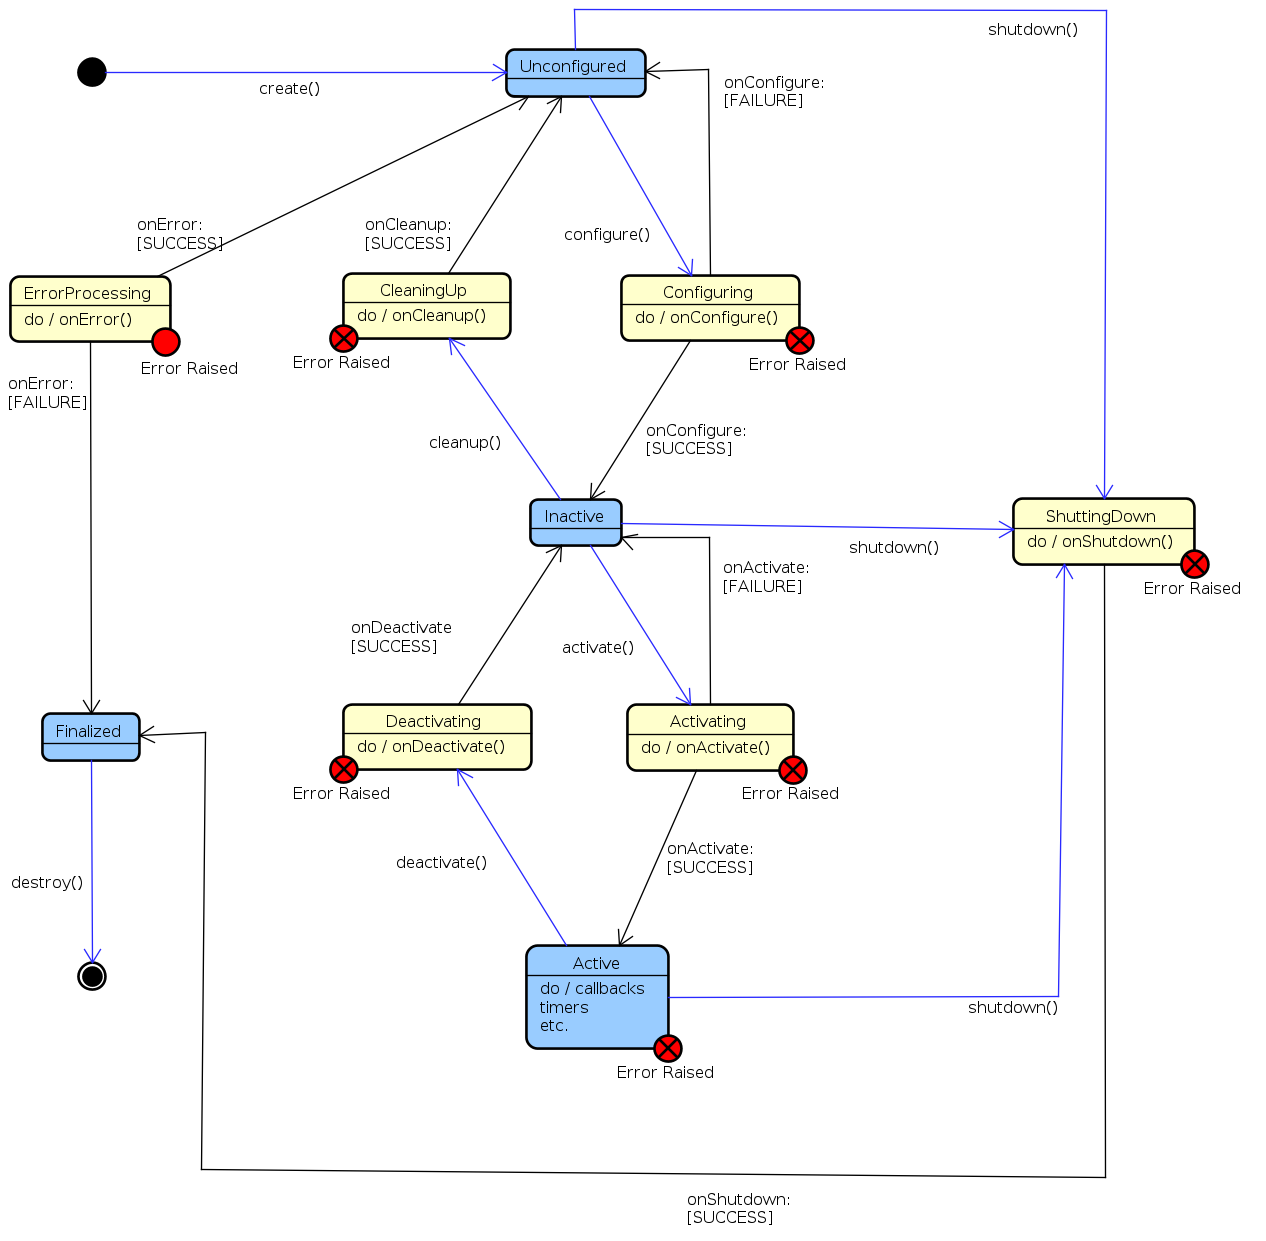
\includegraphics[width=1\linewidth]{img/life_cycle_sm_nf.png}
	\captionof{figure}{State Machine of LifecycleNode}
	\end{figure}\\
	Nodes can also be composed within the same process using the \textbf{Composition}\label{Composition} feature, which improves performance by bypassing middleware overhead\cite{macenski2023impactros2node}.
	\item \textbf{Topics}: Topics are used for communication between nodes to share streams of messages in a publisher-subscriber structure.
	\begin{center}
		\captionsetup{type=figure}
		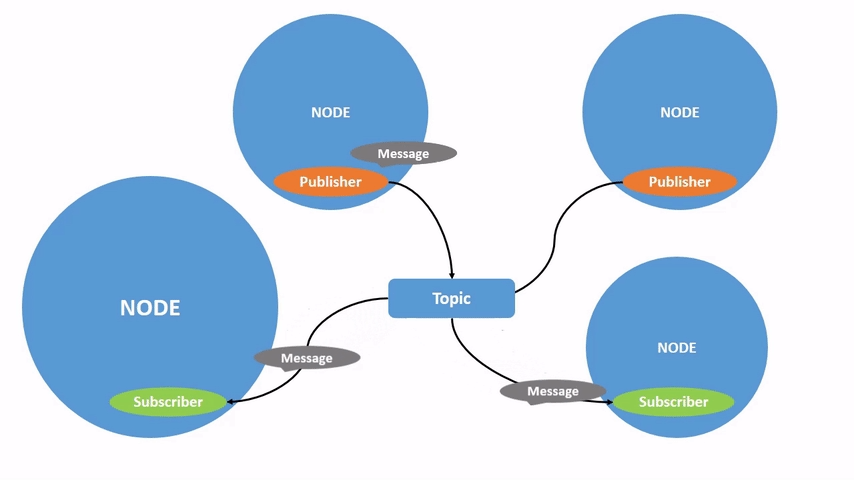
\includegraphics[width=0.6\linewidth]{img/Topic.png}
		\captionof{figure}{Topic process}
	\end{center}
	\item \textbf{Service}: Services are based on the request-response model. When a node with a service client sends a Request Message to a node with a service server, it receives a Response Message from that specific server.
	\begin{center}
		\captionsetup{type=figure}
		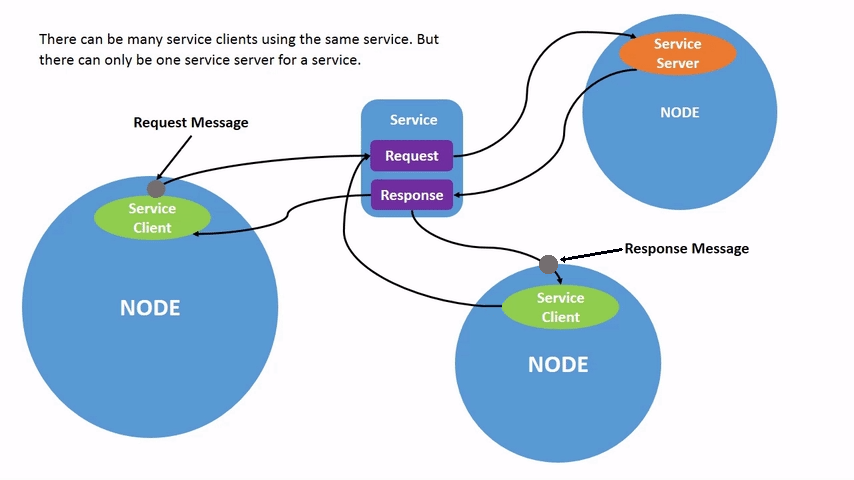
\includegraphics[width=0.6\linewidth]{img/Service.png}
		\captionof{figure}{Service process}
	\end{center}
	\item \textbf{Parameters}: Parameters are configurations of a node that can be modified without changing the source code.
	\item \textbf{Actions}\label{Action}: Actions are designed to support long-running tasks that require feedback and the capability to interrupt when needed. They combine two services (goal and result) and a publisher-subscriber mechanism (feedback). A node sends a goal request and receives an acknowledgment, then starts publishing feedback messages while executing the task, and finally the action server responds with the result.
	\begin{center}
		\captionsetup{type=figure}
		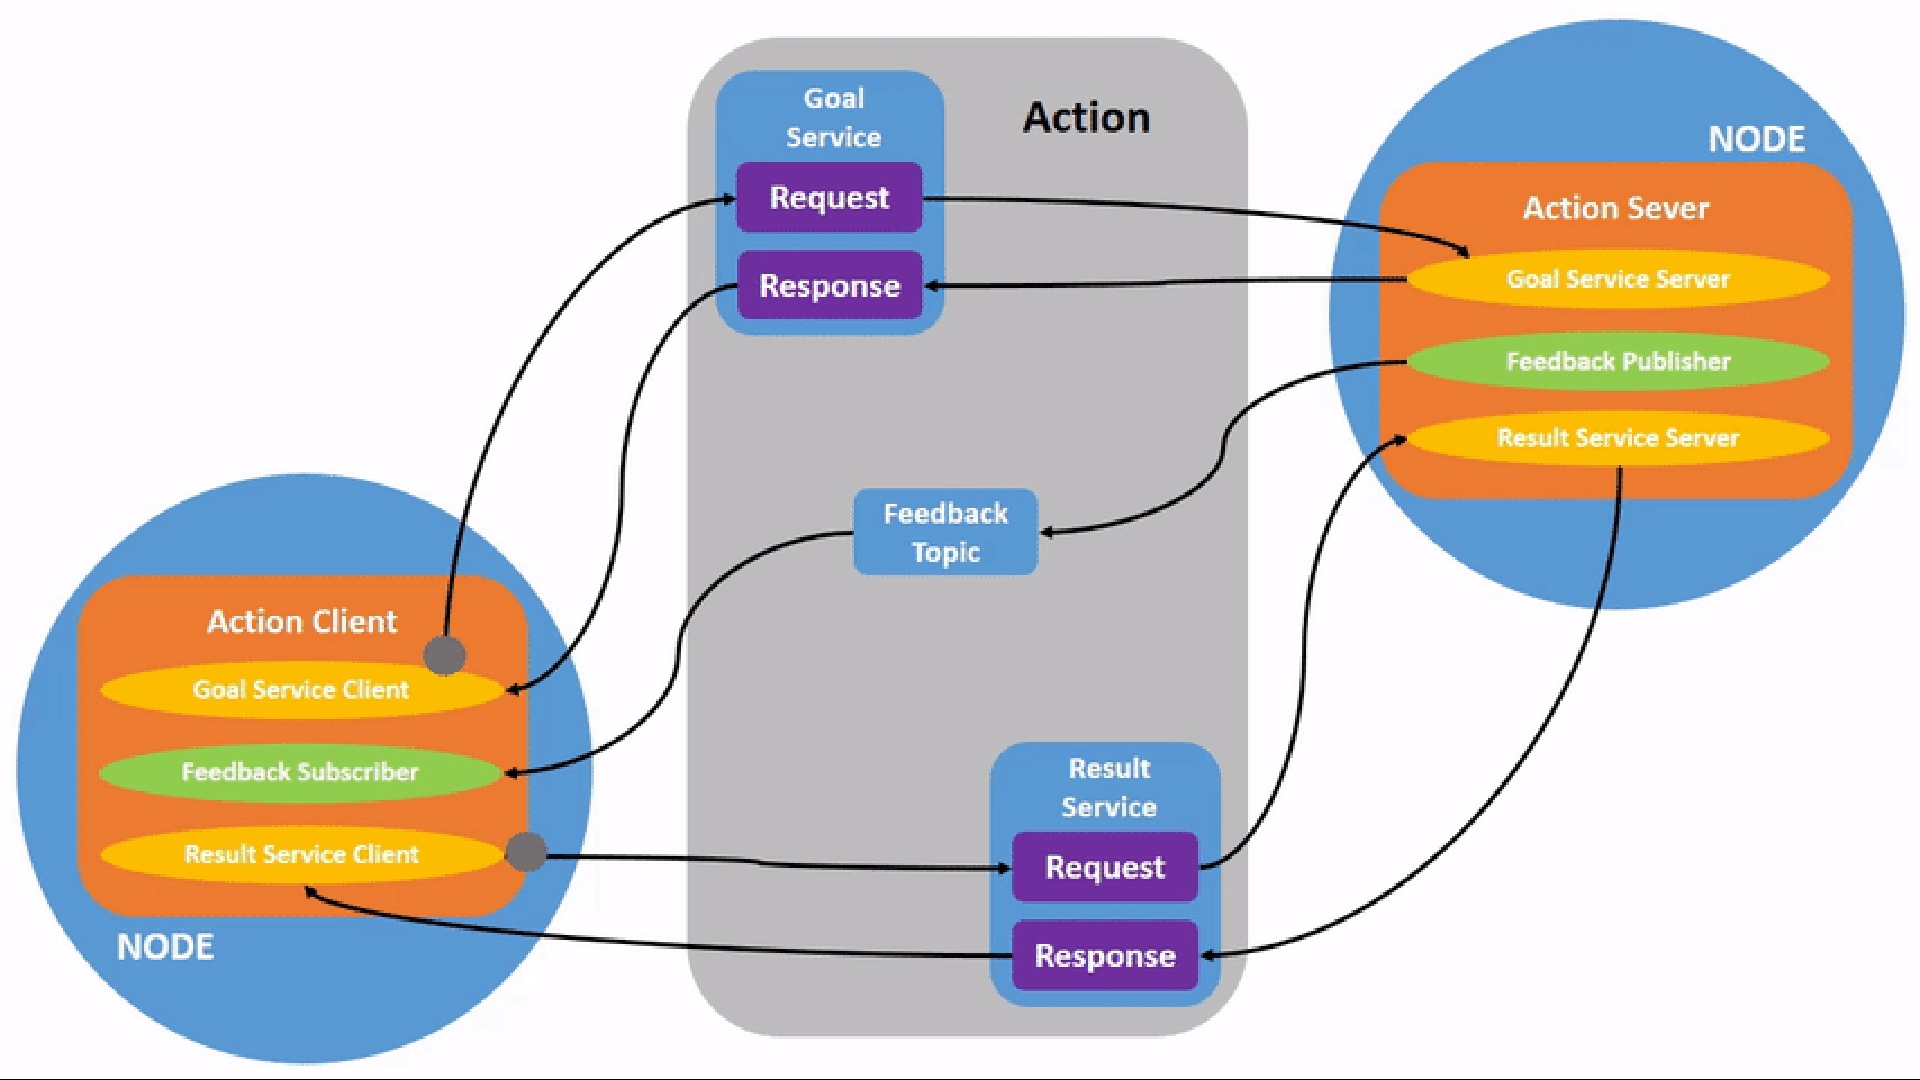
\includegraphics[width=0.6\linewidth]{img/Action.png}
		\captionof{figure}{Action process}
	\end{center}
\end{itemize}
\section{Tools of ROS}
This section describes the tools available in ROS for developing robotic systems:
\begin{itemize}
	\item \textbf{Launch}: A file structure that allows the simultaneous start of multiple nodes with a set of parameters.
	\item \textbf{rqt}: A graphical user interface (GUI) tool for ROS. It includes a series of plugins that facilitate development, monitoring, and diagnostics of the ROS system.
	\item \textbf{Rviz}: A 3D visualization tool for the Robot Operating System. It allows visualization of sensor data and state information from ROS.\\\\
	\begin{figure}[h]
		\centering
		\begin{subfigure}{0.4\textwidth}
		\centering
		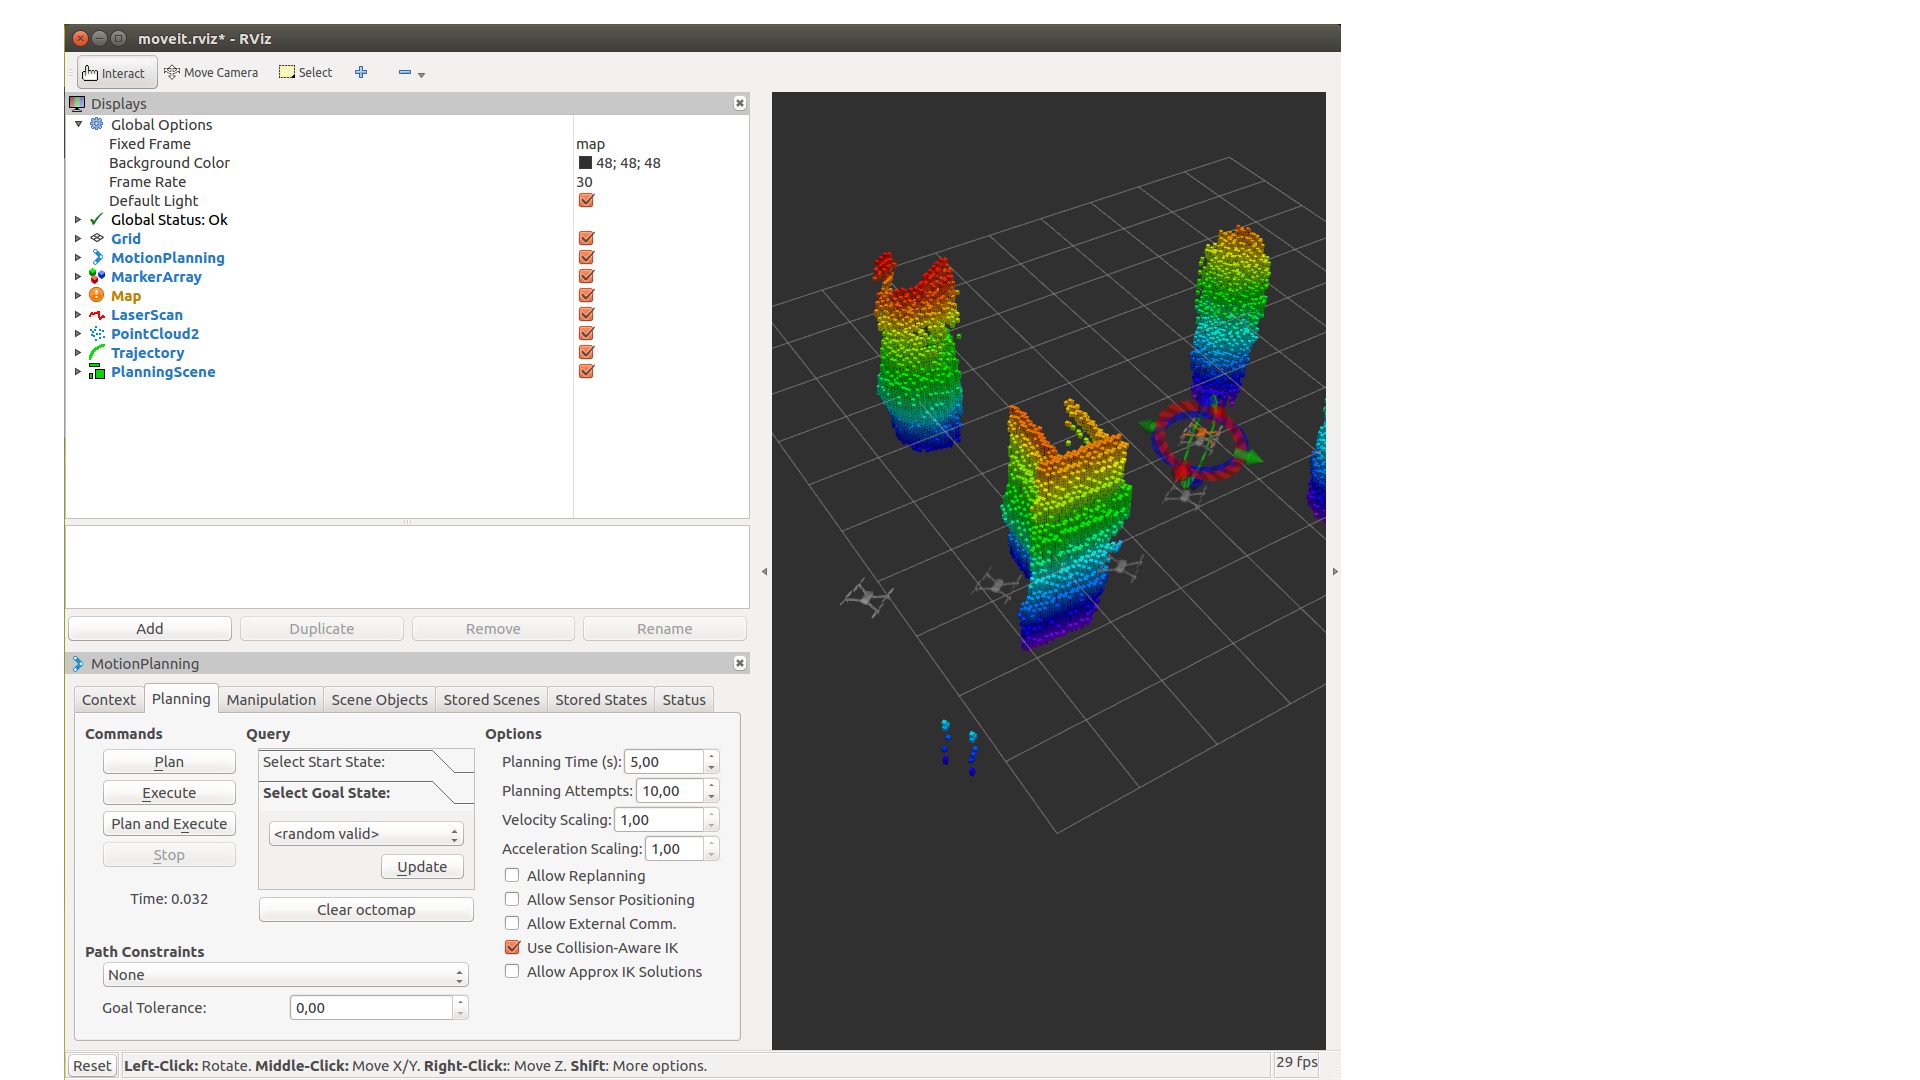
\includegraphics[width=1\linewidth]{img/rviz.png}
		\end{subfigure}
		\begin{subfigure}{0.4\textwidth}
		\centering
		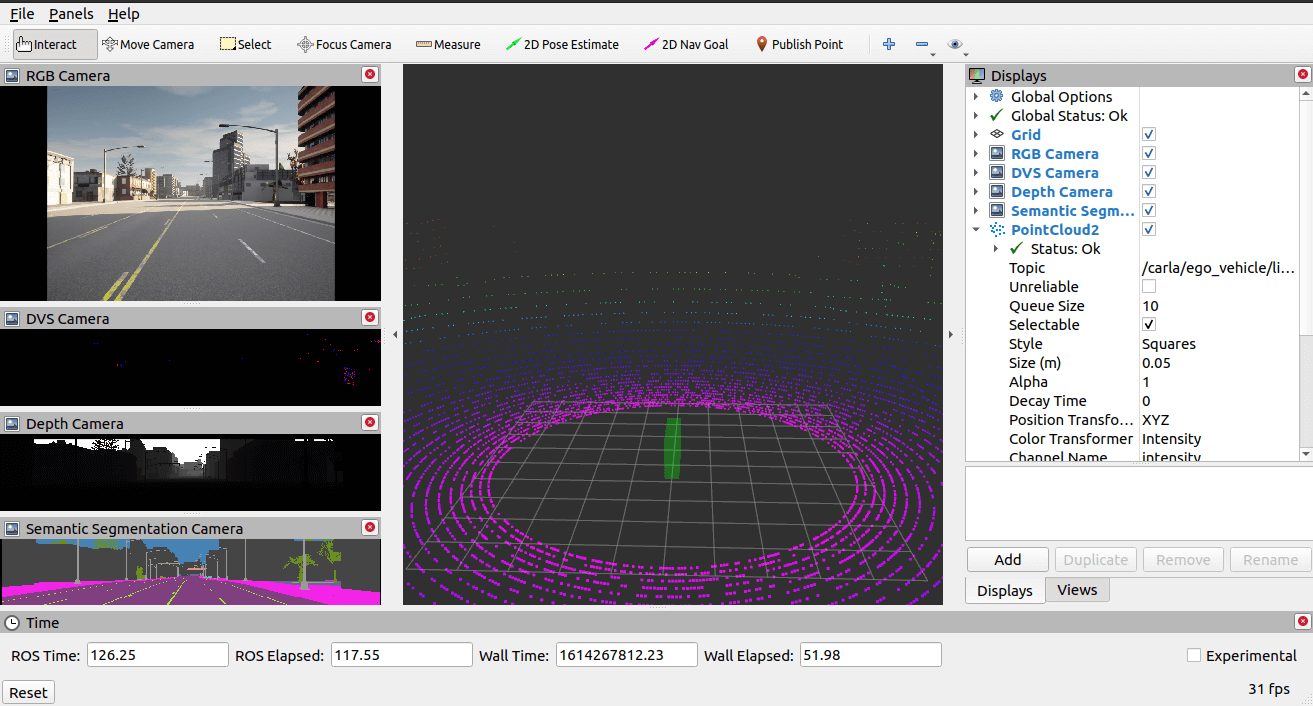
\includegraphics[width=1\linewidth]{img/rviz2.png}
		\end{subfigure}
		\captionof{figure}{Examples of visualization of ROS data with Rviz}
	\end{figure}\\
	\item \textbf{rosdep}: A command-line utility for installing system dependencies required by ROS packages.
	\item \textbf{sros2}: A security extension for ROS 2 that provides tools and instructions to apply security policies to DDS (Data Distribution Service).
\end{itemize}
Another important category of tools that are integrated with ROS is simulation environments. These environments allow developers to test their code on simulated robots under various conditions, which helps identify bugs that could potentially harm a real robot or its environment. Simulation tools provide realistic physical behavior for all components of a robotic system.
According to the ROS documentation, two main simulation tools are commonly used: Gazebo and Webots. Among them, Gazebo is also maintained by Open Robotics and is widely adopted in many projects, including the one discussed in this thesis.\\
Gazebo offer:
\begin{itemize}
	\item \textbf{ROS Integration}: A bridge that converts Protobuf messages to ROS messages, enabling communication between Gazebo and ROS.
	\item \textbf{Performance tools}: Features for distributed simulation across servers, dynamic asset loading, and adjustable time steps to optimize simulation performance.
	\item \textbf{Realistic simulation}: Support for a variety of sensors, including their noise models, within a 3D world rendered using OGRE 2.1\footnote{\href{https://wiki.ogre3d.org/Home}{https://wiki.ogre3d.org/Home}} and powered by multiple physics engine, the default one is DART\footnote{\href{https://dartsim.github.io/}{https://dartsim.github.io/}}.
	\item \textbf{Extensibility}: A modular design that supports plugins, allowing developers to run custom code that interacts directly with the simulation environment.	
\end{itemize}
	\begin{figure}[h]
		\centering
		\begin{subfigure}{0.4\textwidth}
			\centering
			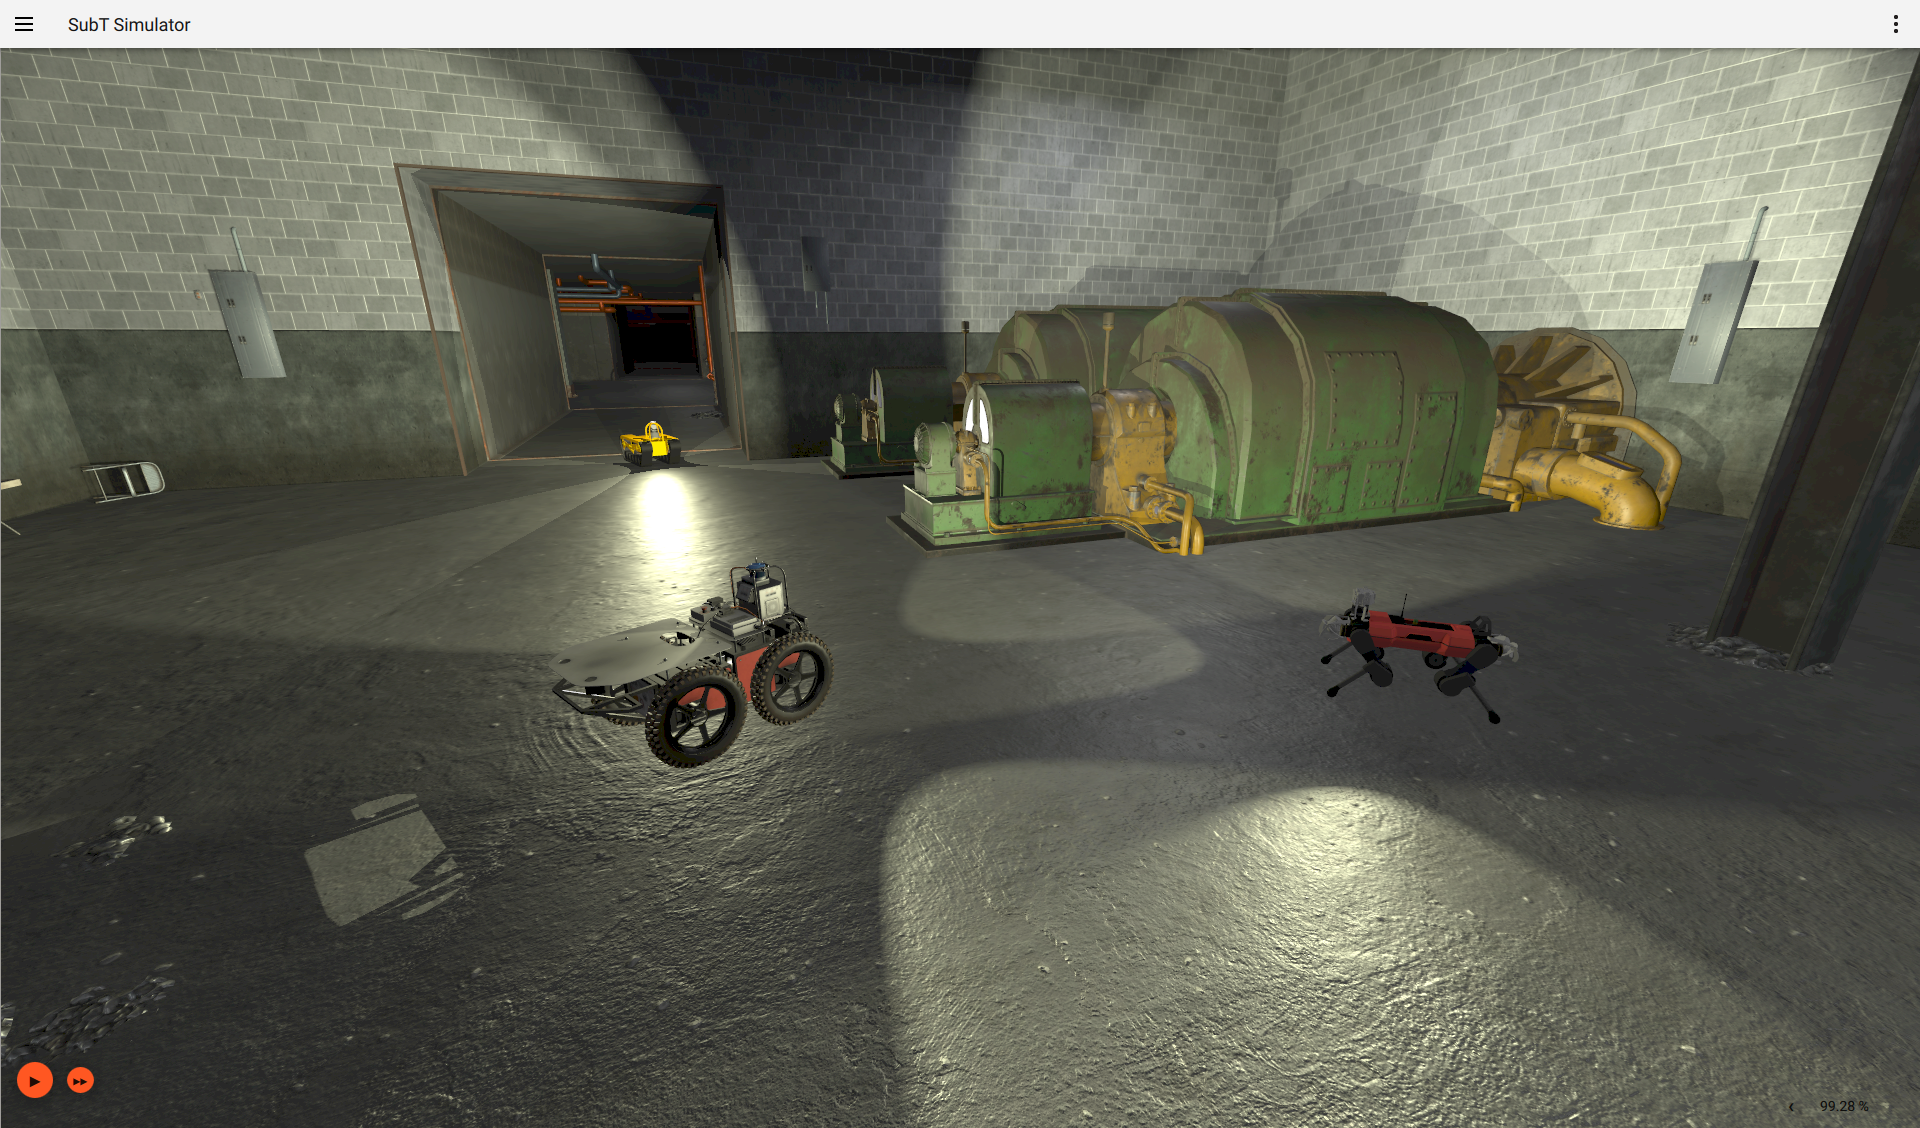
\includegraphics[width=1\linewidth]{img/gazebo1.png}
		\end{subfigure}
		\begin{subfigure}{0.4\textwidth}
			\centering
			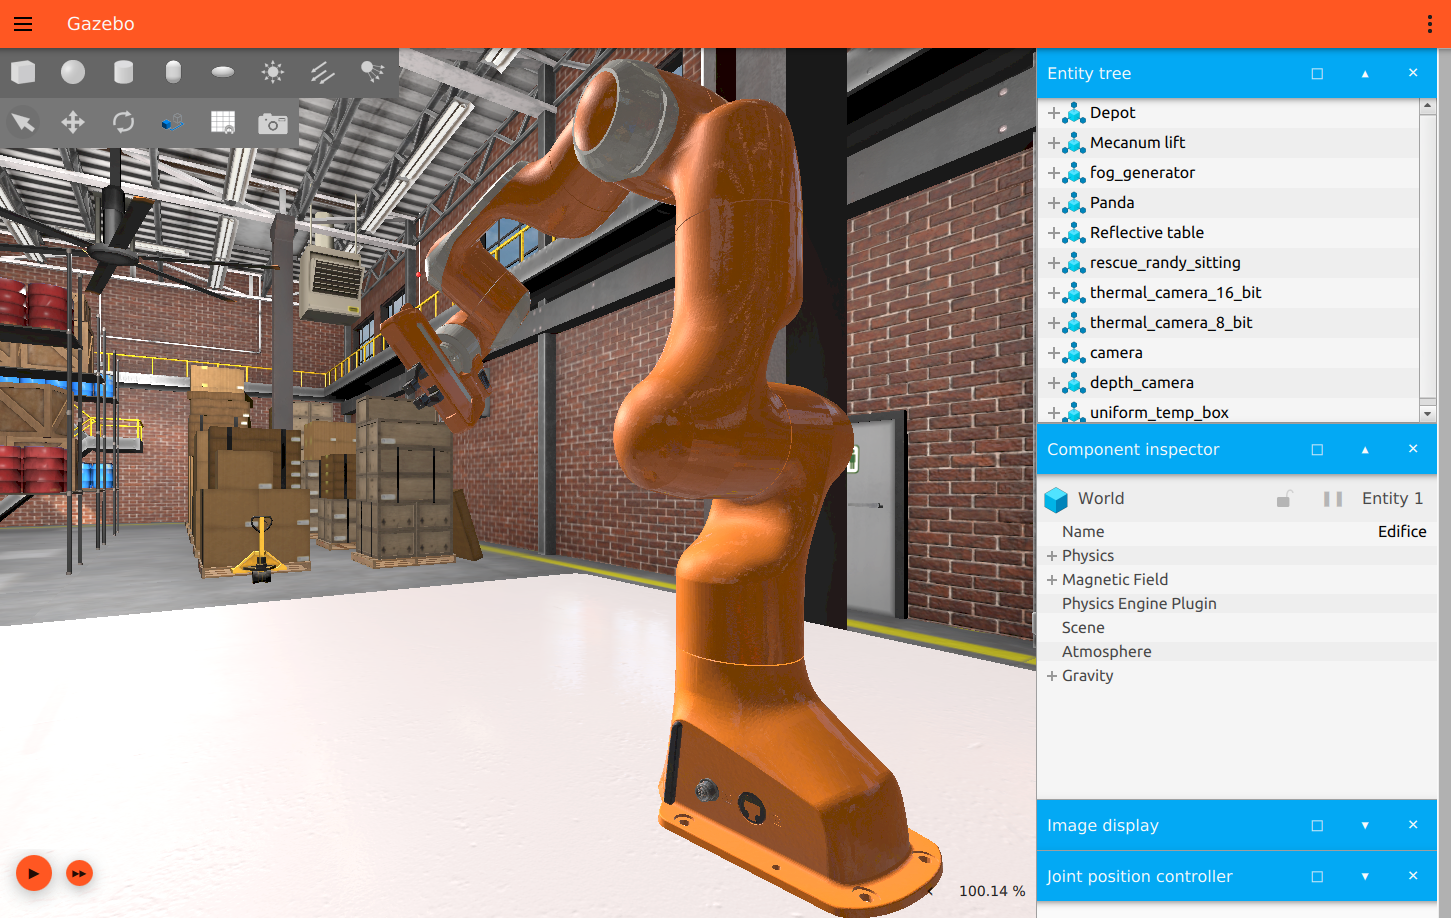
\includegraphics[width=1\linewidth]{img/gazebo2.png}
		\end{subfigure}
		\captionof{figure}{Examples of Gazebo}
\end{figure}
\chapter{Introduction to NAV2 and Google Cartographer}
Multiple tools are available to enable a robot to move autonomously within an environment. One of the most complete systems is Nav2 
\footnote{\href{https://nav2.org/}{https://nav2.org/}}
\cite{macenski2020marathon2}, the successor to the ROS 1 Navigation Stack.
\section{Description of Nav2}
Nav2 provides a comprehensive set of tools for perception, planning\cite{macenski2023survey}, control, localization, and visualization, allowing any robot to navigate autonomously and reliably, even in complex environments. It enables building a model of the environment from sensor data, dynamically calculating the optimal path to avoid obstacles, setting motor velocities, and executing navigation tasks using Behavior Trees.
\begin{figure}[h]
\centering
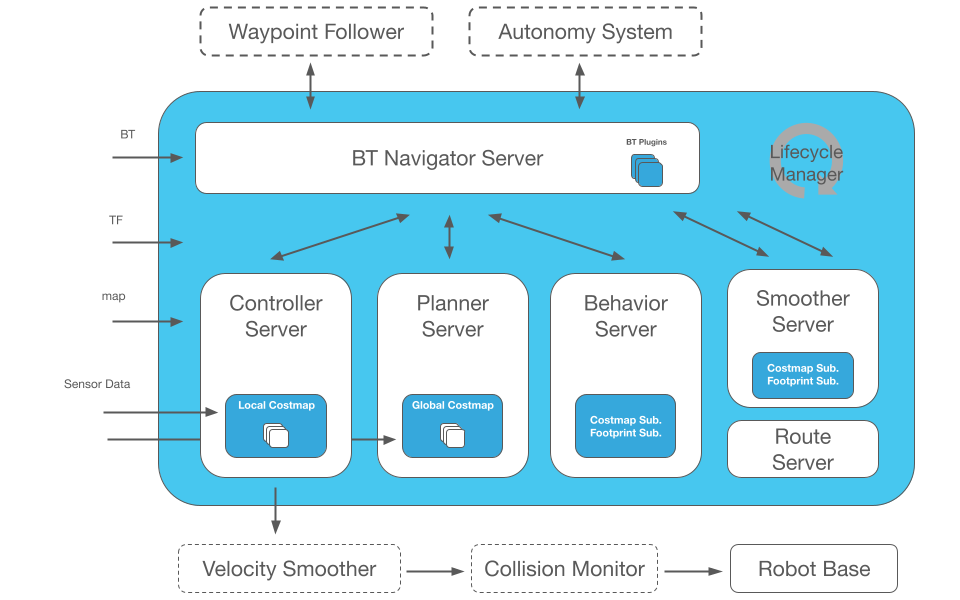
\includegraphics[width=0.8\linewidth]{img/nav2_architecture.png}
\captionof{figure}{Nav2 architecture} \label{Nav2Arch}
\end{figure}
\newpage
Nav2 introduces several improvements over ROS 1, including:
\begin{itemize}
	\item \textbf{Behavior trees}\cite{Colledanchise_2018}: Nav2 uses Behavior Trees to structure and execute tasks in a human-readable and modular way. These trees enable the creation of complex systems and can be tested with various tools. The  BehaviorTree.CPP\footnote{\href{https://www.behaviortree.dev/}{https://www.behaviortree.dev/}} library is used to implement them, and it allows linking different trees for flexible behavior management.
	\item \textbf{nav2\_util LifecycleNode}: This is a wrapper around the standard\\ \texttt{rclcpp\_lifecycle::LifecycleNode} described earlier \ref{LifecycleNode}. It adds a bond connection to the Lifecycle Manager, which monitors the state of each node and can safely transition nodes through their lifecycle states in the event of a failure.
	\item \textbf{Action Server}: Described in \ref{Action}, Nav2 uses action servers for Behavior Tree interactions, such as NavigationToPose (navigate to a specific location) and NavigationThroughPoses (navigate through multiple waypoints).
\end{itemize}
Nav2 is composed of several key nodes that work together to control the robot:
\begin{itemize}
	\item \textbf{Controller Server}: Handles movement requests. It uses plugin-based modules such as a progress checker (to verify if the robot is making progress), goal checker (to determine if the robot has reached its destination), and a controller (to generate velocity commands using the \textbf{local costmap} while avoiding collisions).
	\item \textbf{Planner Server}: Computes the global path to the destination using sensor data and a  plugin-based global planner loaded with the \textbf{global costmap}.
	\item \textbf{BT Navigator Server}: Implements the NavigateToPose, NavigateThroughPoses, and other task interfaces. It is a Behavior Tree-based implementation of navigation that is intended to allow for flexibility in the navigation task and provide a way to easily specify complex robot behaviors.
	\begin{figure}[h]
		\centering
		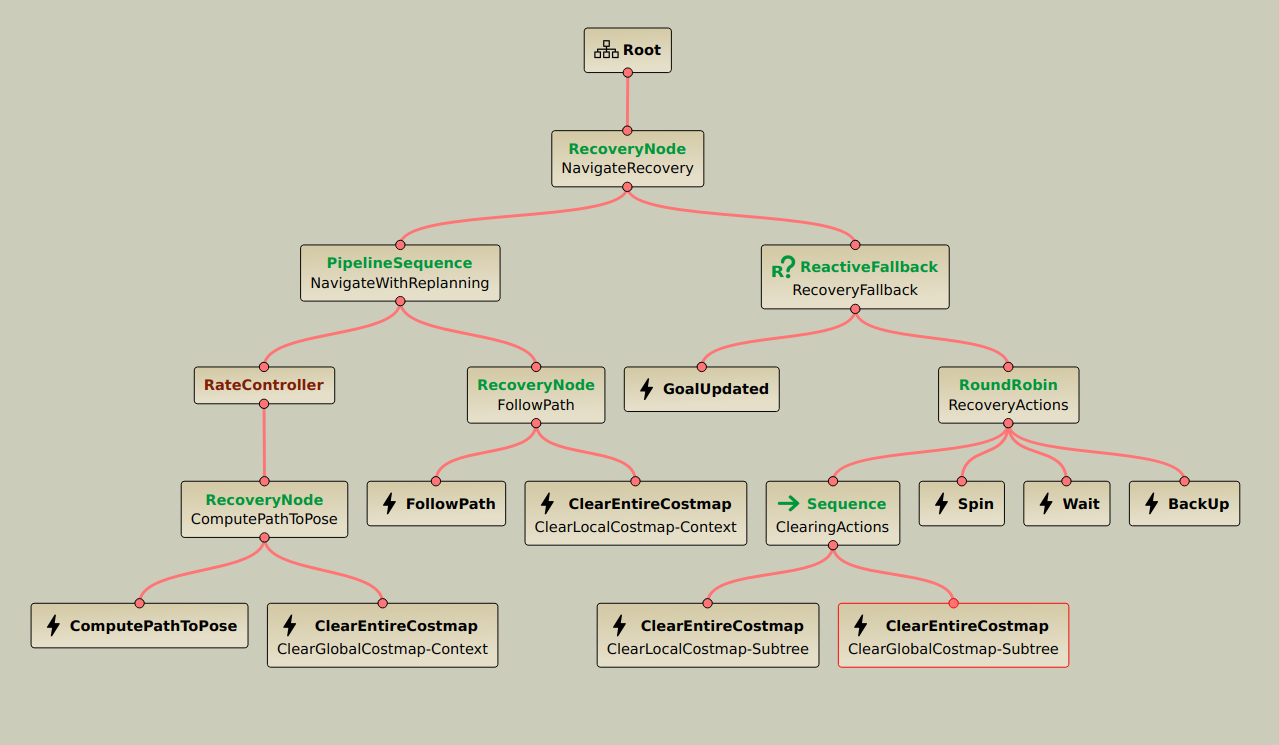
\includegraphics[width=0.72\linewidth]{img/bt_nav2_neg.humble.png}
		\captionof{figure}{Humble Nav2 BT navigation \texttt{navigate\_to\_pose\_w\_replanning\_and\_recovery.xml} loaded with Groot2}
	\end{figure}
	\item \textbf{Smoother Server}: Smooth the path minimizing sharp turns and rapid rotations.
	\item \textbf{Behavior Server}: Handles specific behavior actions like spinning, backing up, and waiting.
	\item \textbf{Waypoint Follower}: An example of orchestrated control (an \textbf{Autonomy System}), this node takes a list of waypoints and uses the NavigateToPose action server to move between them, optionally performing custom tasks (e.g., taking a photo) at each waypoint through plugins.
	\item \textbf{Route Server}: Calculates routes through a predefined navigation graph instead of using free-space planning.
	\item \textbf{Velocity Smoother}: Smooths velocity, acceleration, and deadband signals sent to the robot to ensure safe and smooth motion.
	\item \textbf{Costmap} is a representation of the environment using a regular 2D grid of cells with a cost (unknown, free, occupied, or inflated) and is used for generate the global plan or to compute local control efforts.
\end{itemize}
The next things that Nav2 relies on for controlling the navigation are:
\begin{itemize}
	\item \textbf{state estimation} of the robot that generate a suitable TF tree\label{TF_tree_nav2}, a tree structure of coordinate frames generated using the transform library\cite{6556373}, based on the \href{https://www.ros.org/reps/rep-0105.html}{REP 105}, that is should provide this structure: \texttt{map} $\rightarrow$ \texttt{odom} $\rightarrow$ \texttt{base\_link}. According to the REP 105 they are defines as:
	\begin{itemize}
		\item \texttt{map} : A world-fixed frame that may change in discrete jumps. It's useful for long-term global reference but not suitable for short-term localization.
		\item \texttt{odom} : A continuous world-fixed frame that may drift over time. It provides short-term local reference.
		\item \texttt{base\_link}: A robot fix frame.
	\end{itemize}
	The \texttt{odom} $\rightarrow$ \texttt{base\_link} link \label{ref_odom_to_base}can be estimated using various sensors. For improved accuracy, we use the \texttt{robot\_localization} package\cite{MooreStouchKeneralizedEkf2014}, which provides nonlinear state estimation using Kalman Filter fusing the robot's odometry and the IMU data.\\
	The \texttt{map} $\rightarrow$ \texttt{odom} link can be generate with a global positioning system like Simultaneous Localization And Mapping (SLAM) method\cite{sh-p1-prelude} or using the one provided by Nav2, Adaptive Monte-Carlo Localization (AMCL). \label{ref_map_to_odom}
	\item \textbf{map} can either be preloaded or built dynamically using a SLAM method. One SLAM method systems is Google Cartographer, which will be described in the next section. It is also the SLAM method that was used to generate the map for navigation.
\end{itemize}
\subsection{Cartographer}
Cartographer\cite{45466} is a SLAM method that operates using two main subsystems: a \textbf{Local SLAM} (called \textbf{Frontend}) that build a series of locally consistent \textbf{submaps} from successive scans and from the pose extrapolator with the possibility that it can drift during acquisition and a \textbf{Global SLAM} (called \textbf{Backend}) that reduces drift by performing loop closure—detecting when the robot has returned to a previously visited location. It uses scan matching against submaps and applies global optimization to align all submaps consistently and build a globally accurate map. Cartographer is capable of achieving mapping accuracy of 5 cm, but it requires extensive parameter tuning to reach optimal performance. 
\begin{figure}[h]
	\centering
	\includegraphics[width=1\linewidth]{img/Alg\_Cartographer.png}
	\captionof{figure}{Cartographer Algorithm}
\end{figure}
\chapter{Review of related work on porting navigation stack from ROS 1 to ROS 2}
The widespread adoption of the Robot Operating System (ROS) has introduced new use cases that were not originally considered during its development. Initially created as an academic project, ROS encountered limitations as users began applying it to more complex scenarios such as fleet management, deployment on embedded boards and microcontrollers, real-time systems, unreliable networks, and industrial applications. These emerging requirements highlighted architectural constraints in ROS 1, ultimately necessitating a complete redesign, which led to the development of ROS 2. Comprehensive documentation for ROS 2 is available at \href{https://design.ros2.org/}{https://design.ros2.org/} . Many companies have adopted the ROS 2 ecosystem, noting improvements in development workflows\cite{Macenski_2022} and in specific subsystems like in  Nav2\cite{macenski2023survey}. New initiatives, such as micro-ROS\footnote{\href{https://micro.ros.org/}{https://micro.ros.org/}}, aim to bring ROS 2 capabilities to microcontrollers. Additionally, features like Node Composition offer improved performance optimization\cite{macenski2023impactros2node} while sros2 allow for a better security\cite{vilches2022sros2usablecybersecurity}.
As outlined in these references, ROS 2 offers substantial advantages over ROS 1, making it the preferred framework for modern robotic applications. With this in mind, we will migrate the global planner using the official ROS 2 documentation\footnote{\href{https://docs.ros.org/en/rolling/How-To-Guides/Migrating-from-ROS1.html}{https://docs.ros.org/en/rolling/How-To-Guides/Migrating-from-ROS1.html}} and various secondary sources \footnote{\href{https://industrial-training-master.readthedocs.io/en/melodic/\_source/session7/ROS1-to-ROS2-porting.html}{https://industrial-training-master.readthedocs.io/en/melodic/\_source/session7/ROS1-to-ROS2-porting.html}}. 

\chapter{Overview of open source fleet management systems, particularly Open-RMF}
Currently, several fleet management systems are available:
\begin{itemize}
	\item \textbf{Isaac Mission Dispatch}\footnote{\href{https://github.com/NVIDIA-ISAAC/isaac_mission_dispatch}{https://github.com/NVIDIA-ISAAC/isaac\_mission\_dispatch}}: A microservice-enabled fleet management system developed by NVIDIA that allows users to submit missions to multiple robots and monitor both robot and mission statuses. It provides connectivity between robots and the fleet management system but does not handle logistics such as task allocation or conflict resolution (e.g., intersecting robot paths). The implementation relies on the VDA5050 protocol, an industry standard for communication between cloud control services and mobile robots, and uses MQTT, a lightweight, publish-subscribe network protocol designed for devices with limited resources and bandwidth.	
	\item \textbf{ROOSTER Fleet Management}\footnote{\href{https://github.com/ROOSTER-fleet-management}{https://github.com/ROOSTER-fleet-management}}:An open-source ROS 1-based project that supports heterogeneous fleet management with task allocation, scheduling, and routing functionalities.
	\item \textbf{Open Robotics Middleware Framework (Open-RMF)}\footnote{\href{https://www.open-rmf.org/}{https://www.open-rmf.org/}}: A free, open-source, and modular system that facilitates interoperability between multiple robot fleets and physical infrastructure such as doors, elevators, and building management systems.
	\item \textbf{Robofleet}\footnote{\href{https://github.com/ut-amrl/robofleet}{https://github.com/ut-amrl/robofleet}}\cite{sikand2021robofleetopensourcecommunication}: An open-source system based on ROS 1 that supports inter-robot communication, remote monitoring, and remote tasking for heterogeneous fleets of ROS-enabled service robots. It is specifically designed to handle network variability and to incorporate security control features.
	\item \alert{\textbf{openTCS}\footnote{\href{https://opentcs.org}{https://opentcs.org}}: open Transportation Control System) is a free control system software for coordinating fleets of automated guided vehicles (AGVs) and mobile robots. It can control any automatic vehicle,independent of their specific characteristics, with communication capabilities. Also, It can manage vehicles of different types and performing different tasks at the same time.}
\end{itemize}
Other frameworks provide the infrastructure needed to initiate fleet control:
\begin{itemize}
	\item \textbf{Transitive Robotics}\footnote{\href{https://transitiverobotics.com/}{https://transitiverobotics.com/}}: An open-source framework for full-stack robotics, designed to simplify the development of capabilities that connect robots, cloud services, and web front-ends through a dynamically updating shared data model. It addresses common challenges in building full-stack robotic applications, such as unreliable networks, intermittently offline robots, and cross-device versioning.
	\item \textbf{Robot Web Tools}\footnote{\href{https://robotwebtools.github.io/}{https://robotwebtools.github.io/}}: A collection of tools that enable communication with remote robots via web technologies, facilitating remote monitoring and interaction.
\end{itemize}
Given that Open-RMF offers control over multiple fleets, enables structured interaction between them to achieve optimal outcomes, provides a comprehensive toolset for system development, is based on ROS 2, and is open source, it will be used as the foundation for our fleet management architecture.
\section{Open-RMF description}
Open-RMF is a flexible and modular toolkit built on ROS 2 that facilitates interaction between heterogeneous robot fleets. It employs standardized protocols to enable communication with infrastructure, environments, and automation systems, optimizing the utilization of critical shared resources such as elevators, doors, narrow corridors, and other robots. By coordinating access to these resources, Open-RMF introduces system-level intelligence that helps prevent conflicts and ensures proper task and resource allocation.
Figure \ref{fig:Open-RMF Structure} illustrates the architecture and operational workflow of Open-RMF.
\begin{figure}[h]
	\centering
	\includegraphics[width=0.8\linewidth]{img/RMF\_struct.png}
	\captionof{figure}{Open-RMF Structure}
	\label{fig:Open-RMF Structure}
\end{figure}
\\
The fleets that can be controlled through Open-RMF can be categorized into three types:
\begin{itemize}
	\item \textit{Full Control}: Fleets of this type provide full status updates and allow complete control over path planning and execution.
	\item \textit{Traffic Light}: These fleets also provide full status updates, but only allow limited control, such as pausing and resuming operations. Open-RMF has control over certain behaviors, but not over the specific paths.
	\item \textit{Read Only}: These fleets only provide status updates and cannot be controlled. Only one read-only fleet can exist in the system at any given time, as the presence of multiple read-only fleets would make it nearly impossible to avoid deadlocks or resource conflicts.
\end{itemize}
If a fleet lacks has \textit{No Interface}, it can lead to deadlocks in resource allocation and is incompatible with an RMF system.
\\
The core of Open-RMF, known as \texttt{rmf\_core}, is composed of several modular packages, each serving a distinct role within the system:
\begin{itemize}
	\item \texttt{rmf\_traffic}: Provides core scheduling and traffic management capabilities. It is based on a platform-agnostic \textbf{Traffic Schedule Database} and includes two main mechanisms for traffic deconfliction:
	\begin{figure}[h]
		\centering
		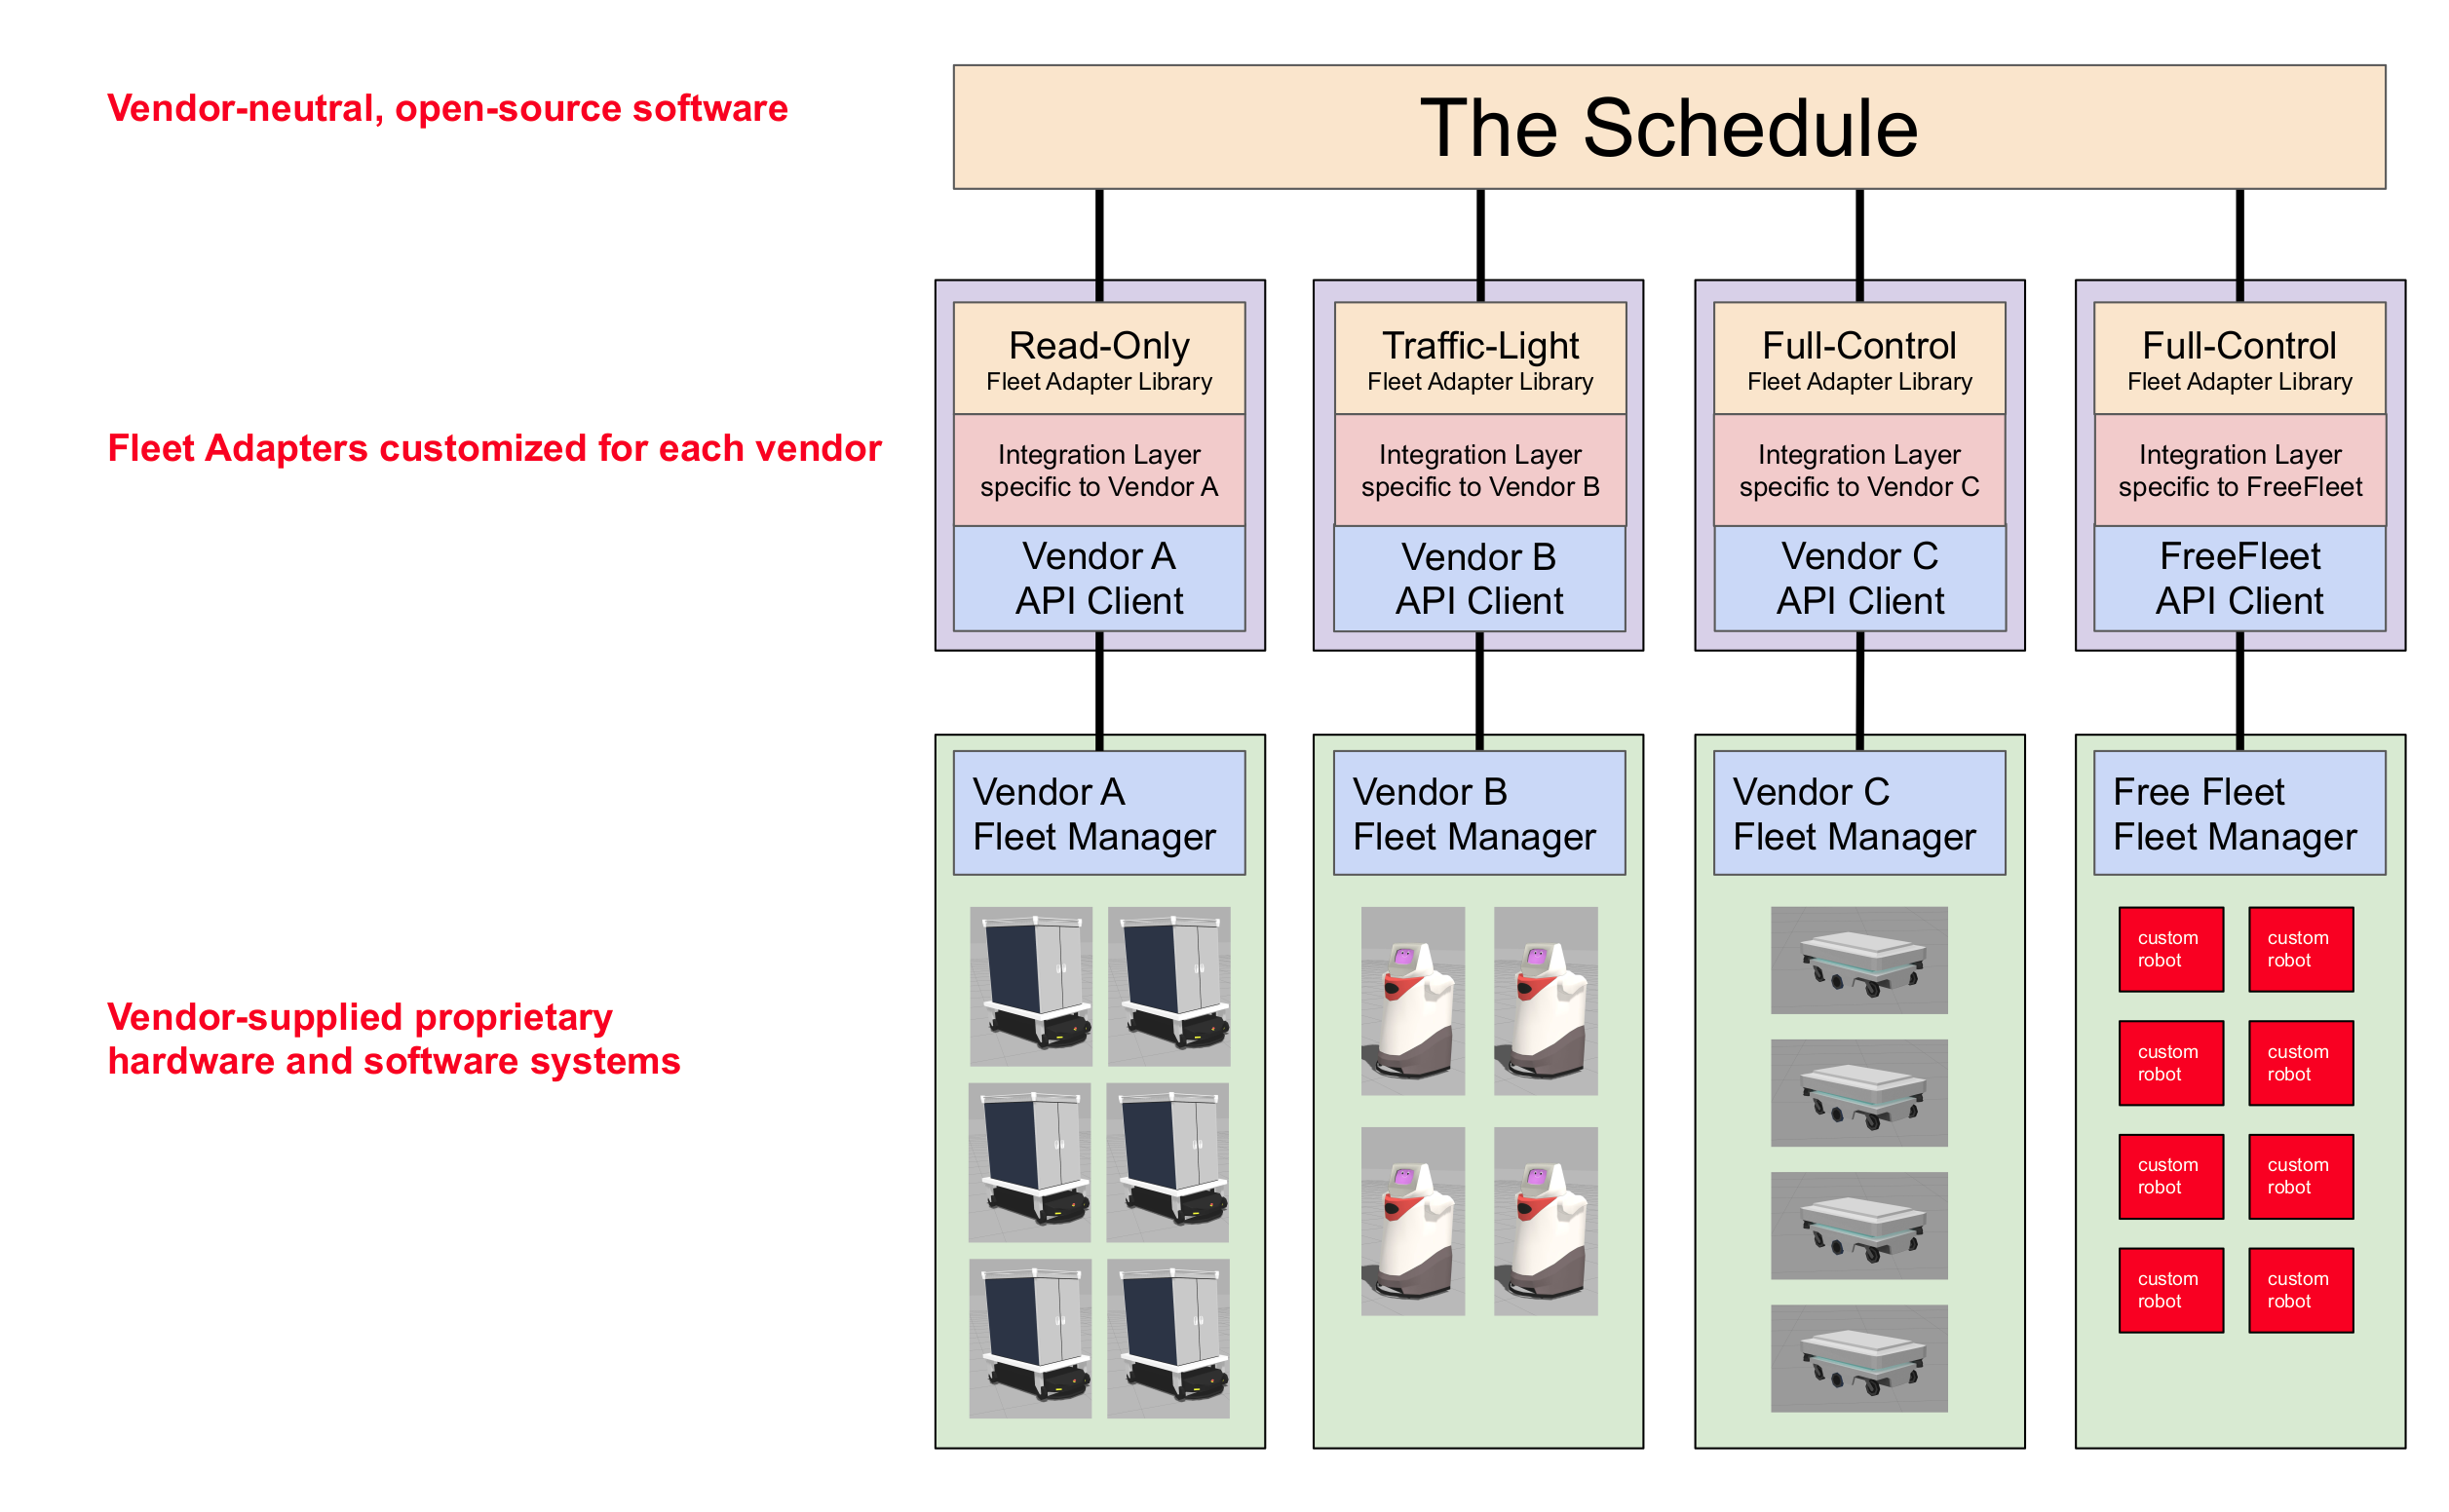
\includegraphics[width=0.8\linewidth]{img/RMF_tut_schedule.png}
		\captionof{figure}{Open-RMF Schedule structure}
		\label{fig:Open-RMF Schedule structure}
	\end{figure}
		\begin{itemize}
			\item \textit{Prevention}: When changes occur in the database (e.g., route cancellations), fleet managers can proactively replan routes to avoid conflicts.
			\item \textit{Negotiation}: When a potential conflict is detected between two or more schedule participants, a conflict notice is issued to the relevant fleet managers. Each manager responds with a preferred path that accommodates other agents, and an external arbitration module selects the optimal path.
		\end{itemize}
	Conflict avoidance for Automated Guided Vehicles (AGVs) is implemented using a time-dependent extension to A* search. This algorithm considers both spatial and temporal dimensions, allowing it to generate conflict-free paths by accounting for the future movements of other agents. Support for Autonomous Mobile Robots (AMRs) is under active development.
	\item \texttt{rmf\_traffic\_ros2}: Provides the necessary ROS 2 interfaces for integrating rmf\_traffic into ROS 2-based systems.
	\item \texttt{rmf\_task}: Contains APIs and base classes for defining and managing tasks in RMF.
	The framework natively supports three types of task requests:
	\begin{itemize}
		\item \textit{Clean}: For robots capable of cleaning floor spaces.
		\item \textit{Delivery}: For robots tasked with transporting items between locations.
		\item \textit{Loop}: For robots required to repeatedly navigate between two or more points.
	\end{itemize}
	\item \texttt{rmf\_dispatcher\_node}: Contains the logic responsible for task allocation and management across multi-fleet systems. When a user submits a new task request, the dispatcher intelligently assigns it to the most suitable robot by querying each fleet adapter capable of performing the task. These adapters respond with bids indicating which robot is best suited, and RMF uses this bidding mechanism to determine the optimal assignment, as illustrated in Figure \ref{fig:Open-RMF Bid Task}.
	\begin{figure}[h]
		\centering
		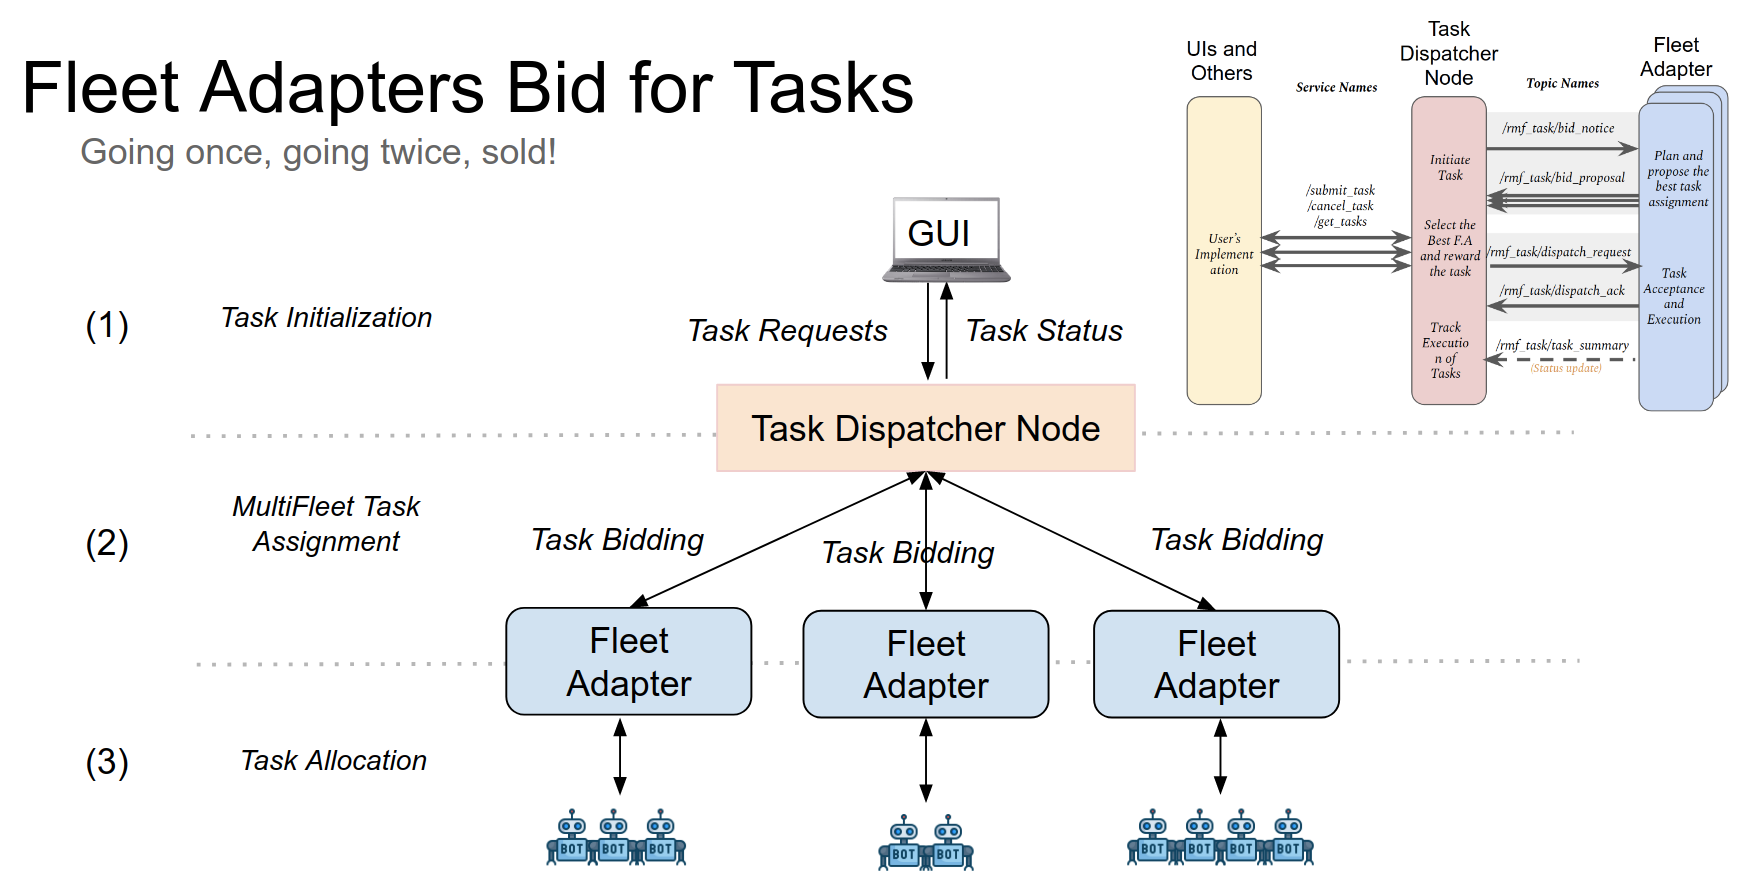
\includegraphics[width=0.8\linewidth]{img/RMF_tut_BidTask.png}
		\captionof{figure}{Open-RMF Bid Task}
		\label{fig:Open-RMF Bid Task}
	\end{figure}
	\item \texttt{rmf\_battery}: Provides battery consumption estimation models for different robot activities, aiding in energy-aware task planning.
	\item \texttt{rmf\_ros2}: Supplies ROS 2 adapters, nodes, and Python bindings to integrate the RMF core components into ROS 2 applications.
	\item \texttt{rmf\_utils}: A collection of utility functions and tools used across various RMF packages.
	
\end{itemize}

The following tools are available to support development with Open-RMF:
\begin{itemize}
	\item \textbf{RMF demos}: A collection of demonstration packages showcasing the capabilities of Open-RMF. These serve as a useful starting point for development and experimentation.
	\item \textbf{Traffic Editor}: A graphical map editor used to define traffic patterns and interaction points (e.g., doors, lifts) that RMF uses for traffic management. It also supports the generation of Gazebo simulation worlds based on the designed maps.\\
	\begin{figure}[h]
		\centering
		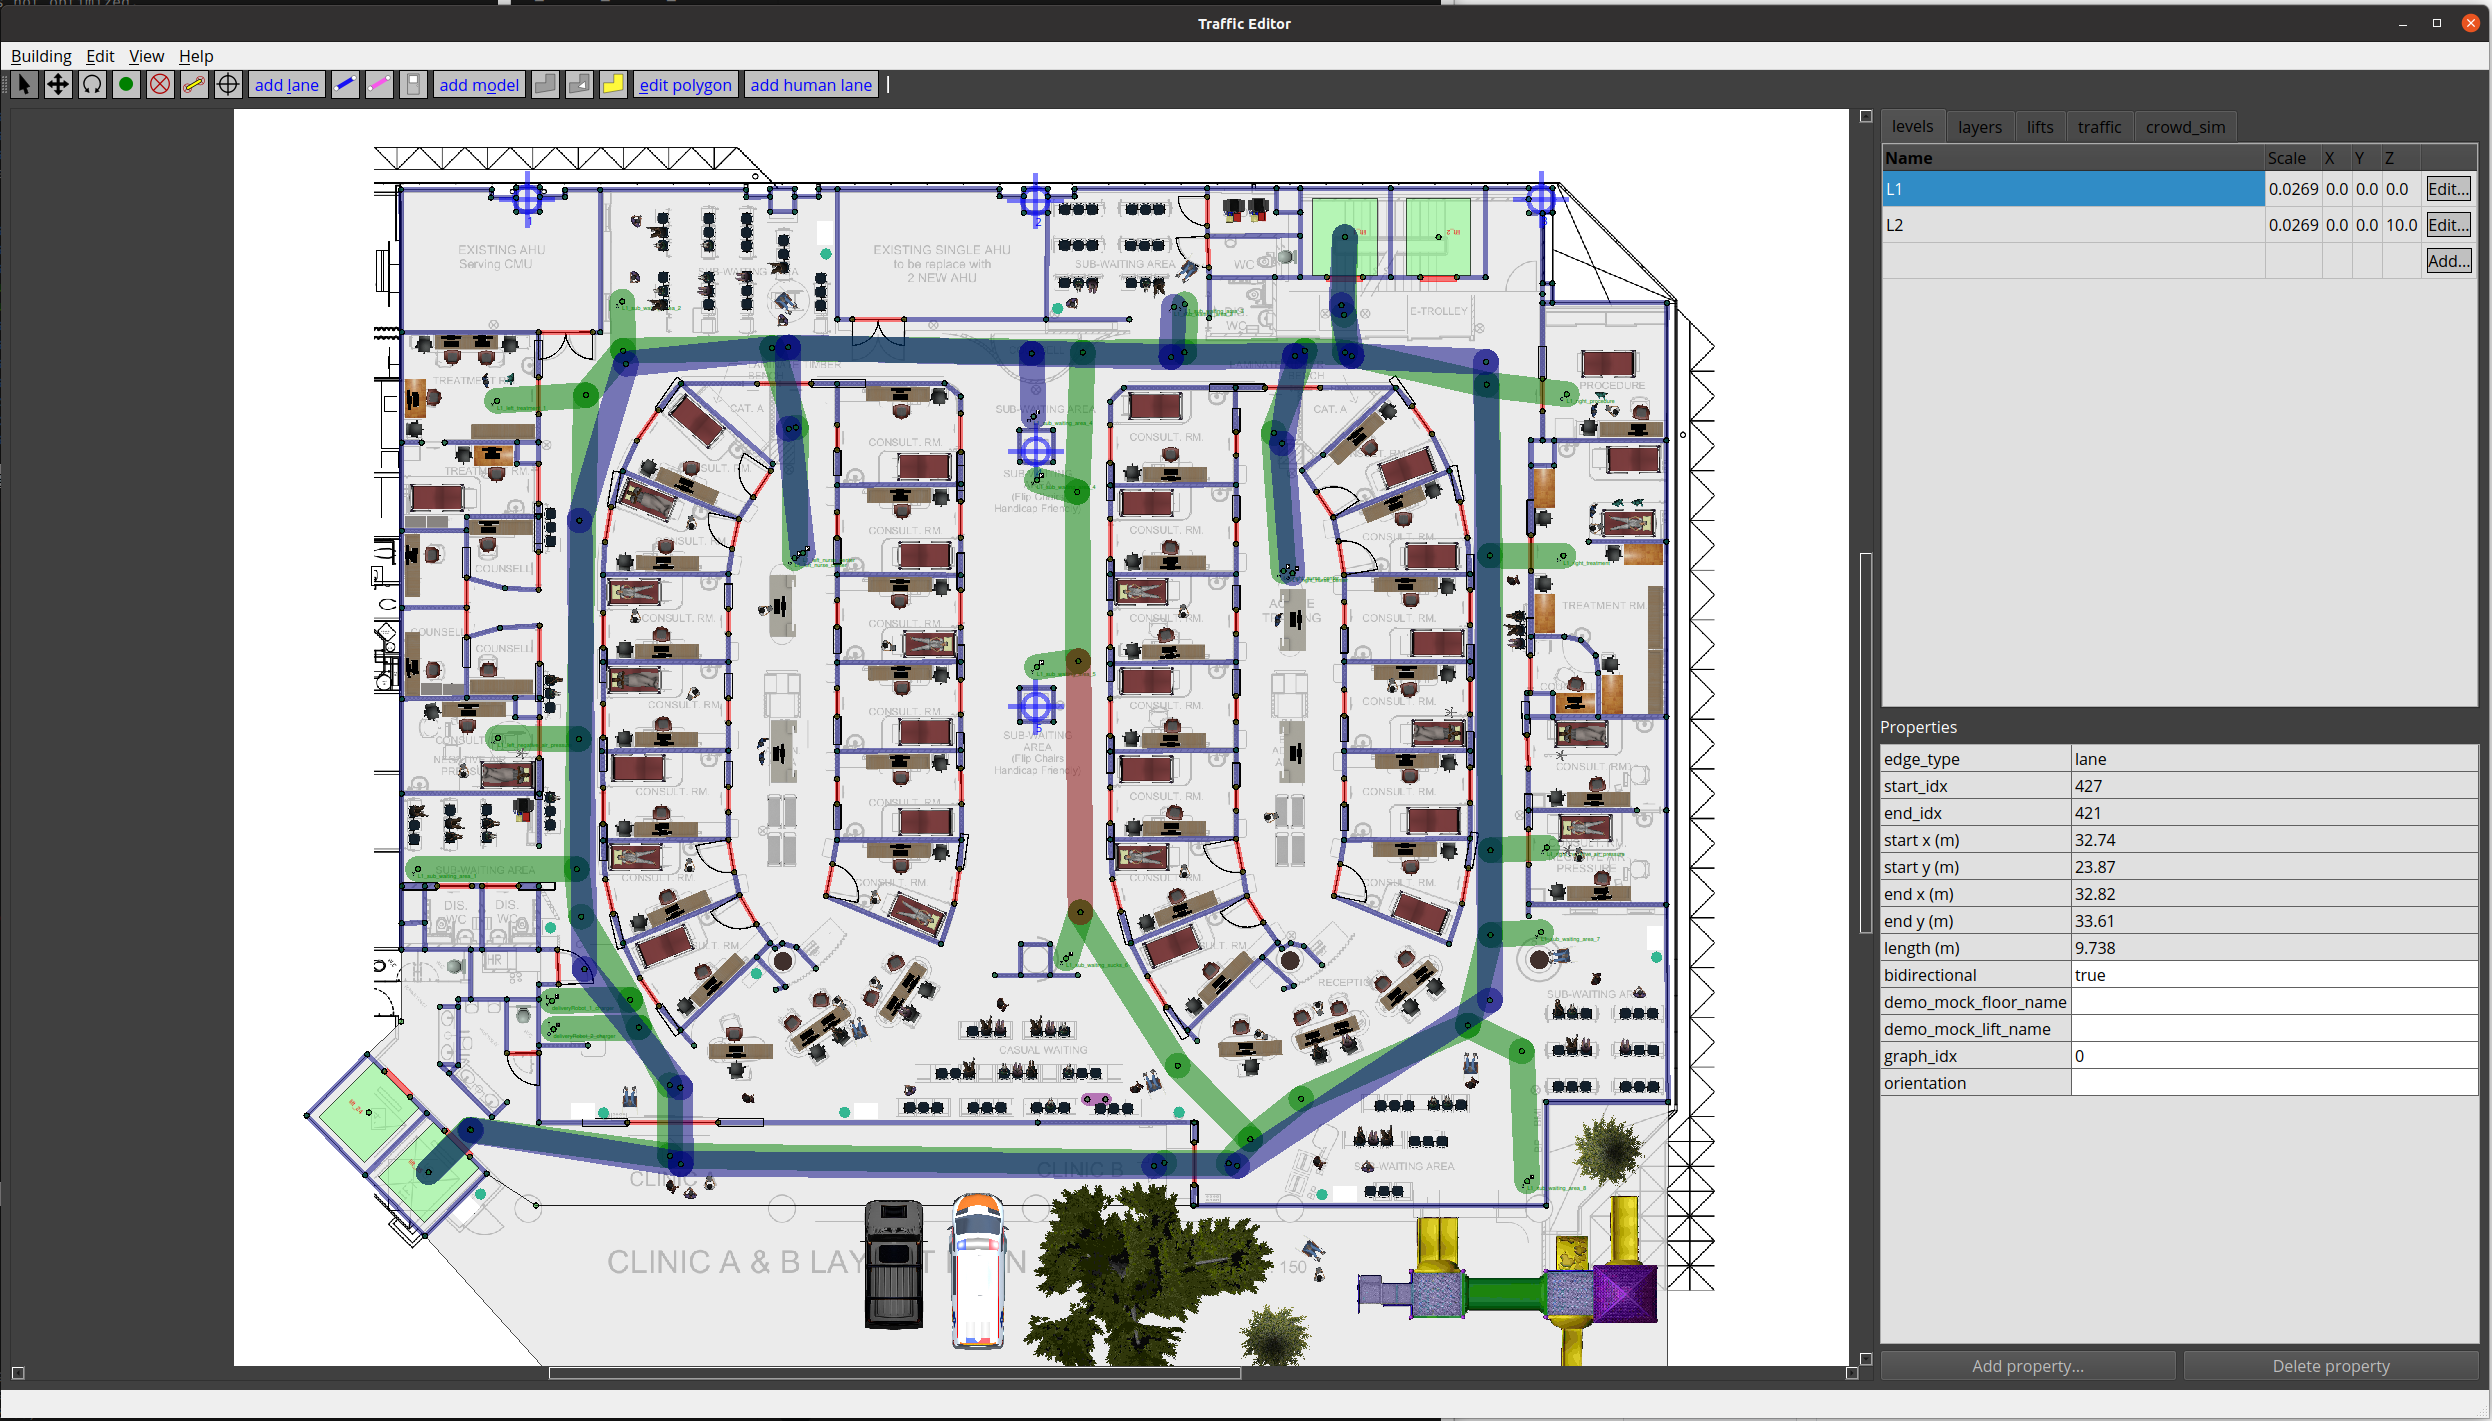
\includegraphics[width=0.8\linewidth]{img/RMF_tut_trafficEditor.png}
		\captionof{figure}{Traffic Editor}
		\label{fig:Traffic Editor}
	\end{figure}\\
	Another version of this software,  \textbf{rmf\_site}\footnote{\href{https://github.com/open-rmf/rmf\_site}{https://github.com/open-rmf/rmf\_site}}, is currently undergoing active deployment.
	\item \textbf{Free Fleet}: An open-source fleet adapter that enables the integration of standalone mobile robots into Open-RMF, allowing the creation of heterogeneous fleets.
	\begin{figure}[h]
		\centering
		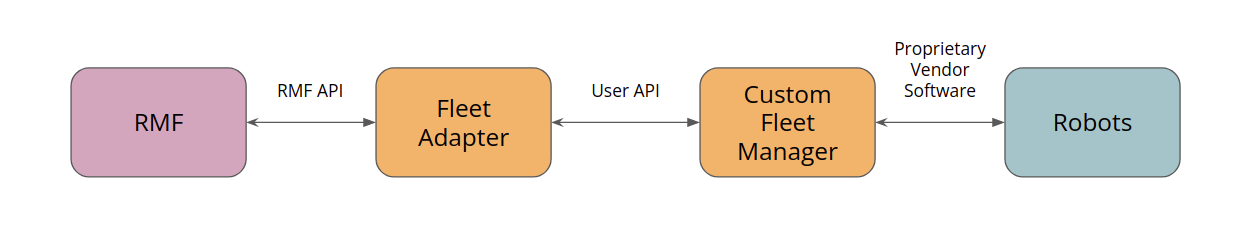
\includegraphics[width=0.8\linewidth]{img/RMF_tut_fleetAdapterTMPL.png}
		\captionof{figure}{Fleet Adapter}
		\label{fig:Fleet Adapter}
	\end{figure}
	\item \textbf{RMF Schedule Visualizer}: An RViz plugin that provides visualization and monitoring of the RMF schedule, enabling users to observe and interact with traffic and task execution in real time.
	\newpage
	\item \textbf{RMF Web UI} : A web-based application for visualization and control of the Robotic Middleware Framework (\texttt{rmf\_core}). It provides a user-friendly interface for monitoring system state and interacting with fleet operations.
	\begin{figure}[h]
		\centering
		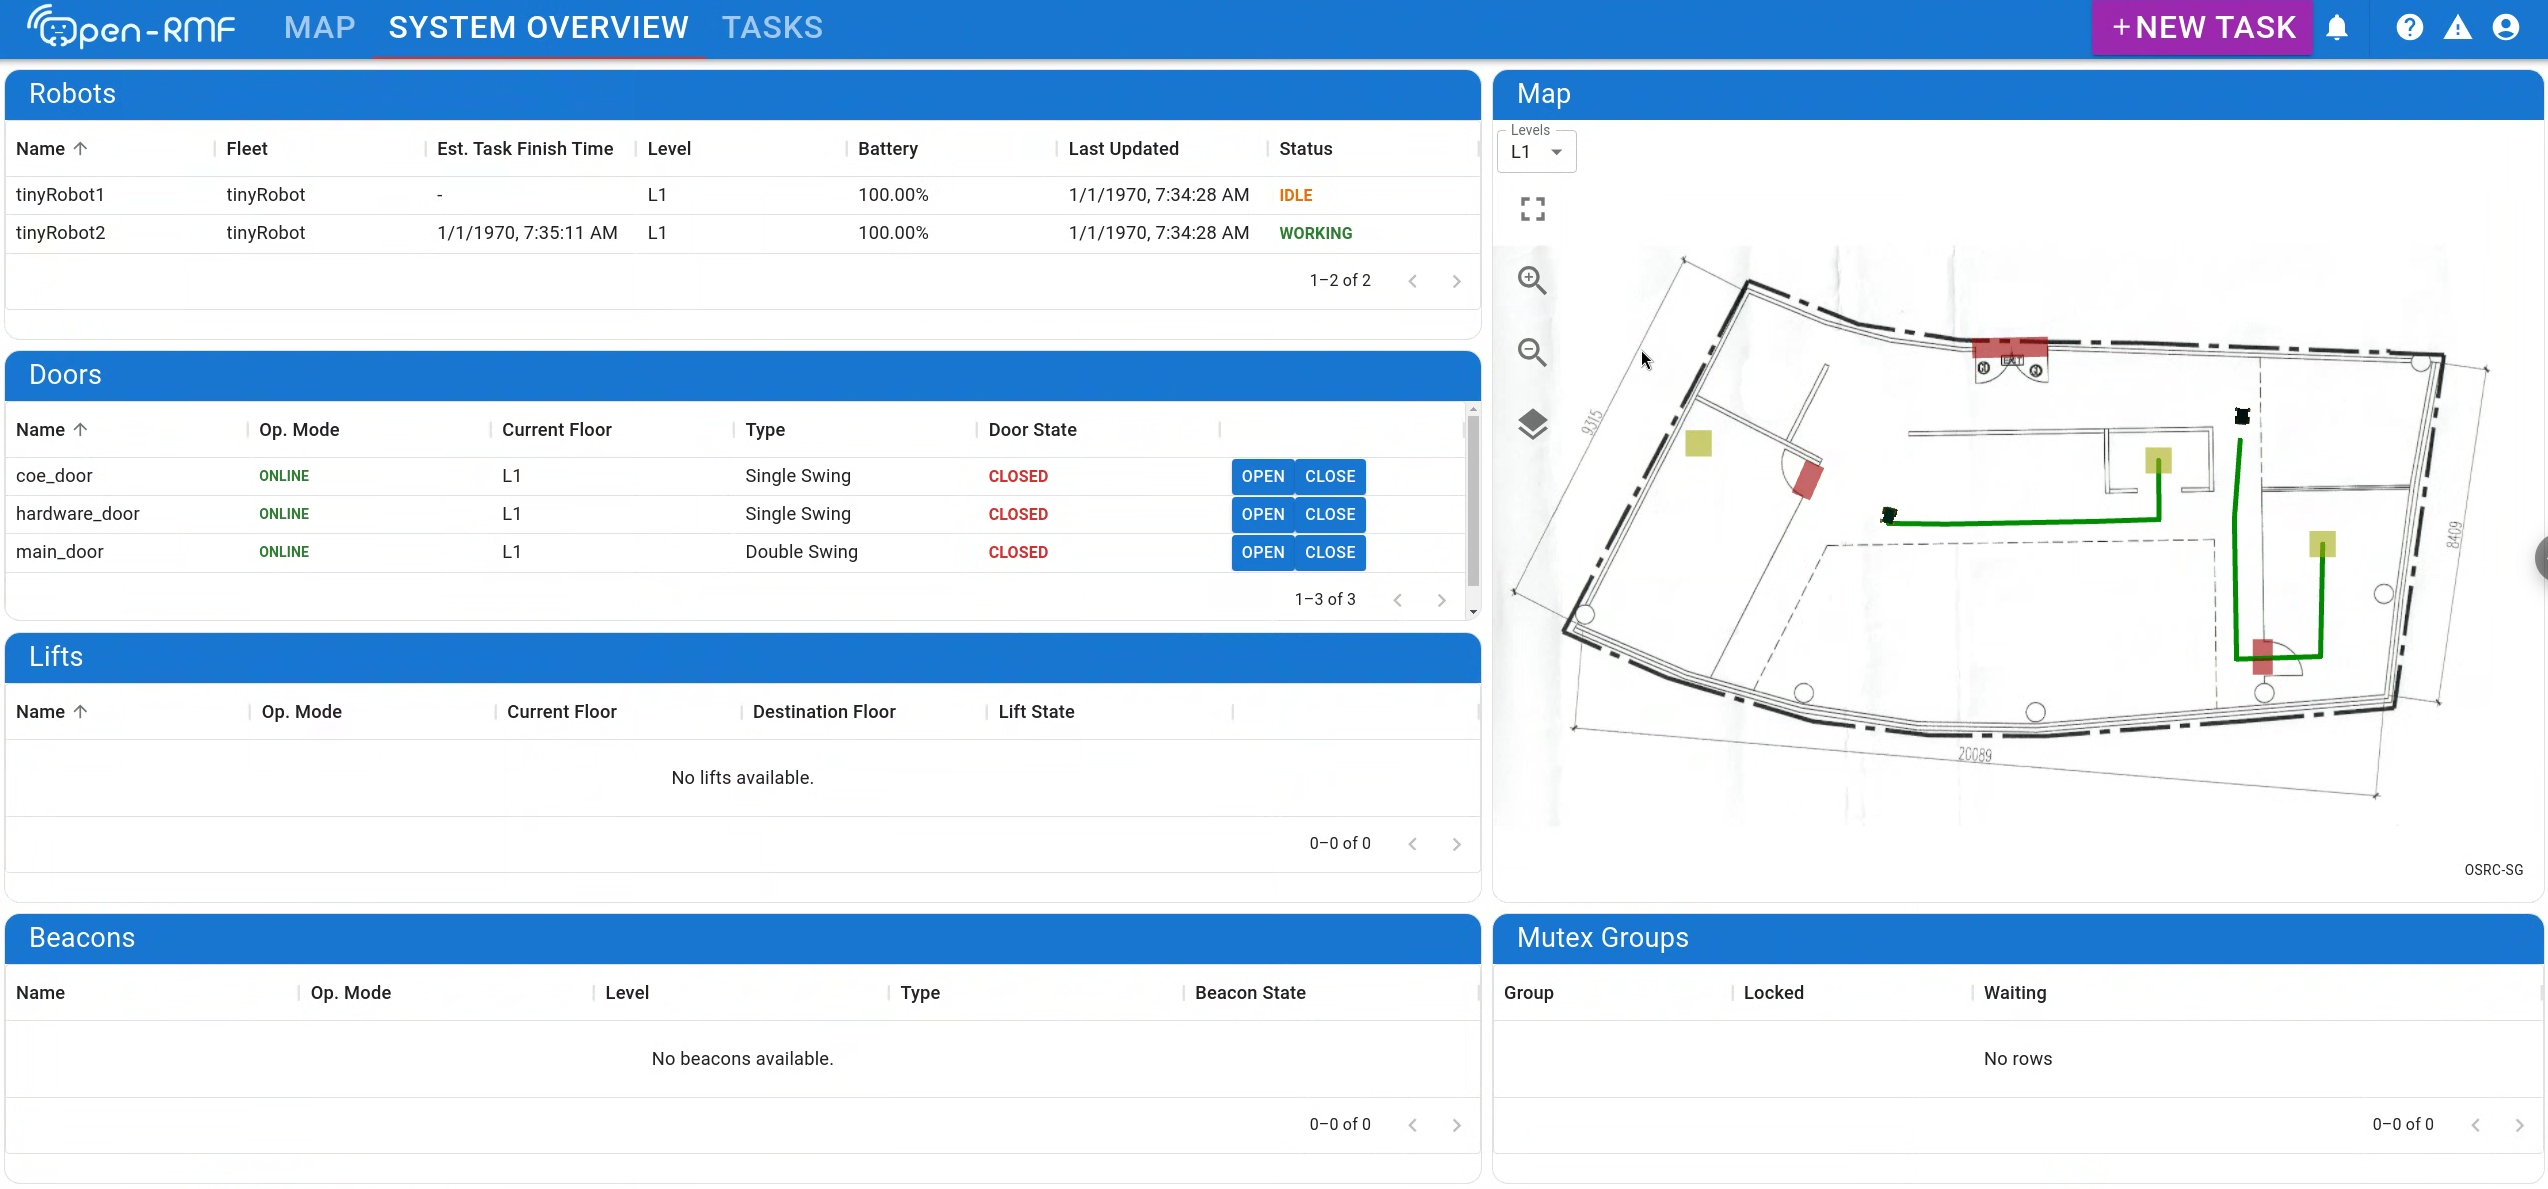
\includegraphics[width=0.8\linewidth]{img/RMF_tut_web.png}
		\captionof{figure}{RMF Web}
		\label{fig:RMF Web}
	\end{figure}
	\item \textbf{RMF Simulation}: A set of Gazebo plugins designed to simulate various aspects of building infrastructure—such as doors, lifts, and crowds—as well as robot behavior, including navigation and interactions with workcells.
	\item \textbf{Simulation assets}: Freely available 3D models and environment assets used to support simulation development and testing in Gazebo.
\end{itemize}


\part{Methodology}
In this part, we describe the entire procedure followed in the development of this project:
\begin{itemize}
	\item The setup of our testing platform, based on the Rover Mini and a suite of onboard sensors.
	\item The configuration of the Nav2 navigation stack.
	\item The procedure used to port the global planner from ROS 1 to ROS 2, and its integration into the Nav2 framework.
	\item The tools and methods used to integrate the system into Open-RMF.
\end{itemize}
All source code developed for this project is publicly available in the following GitHub repository: \texttt{michbelle/myTesiCode}\footnote{\href{https://github.com/michbelle/myTesiCode}{https://github.com/michbelle/myTesiCode}}. The repository also includes the necessary components for simulating the system.\\
The simulation environment is containerized using Docker, which provides a consistent and OS-independent base system. The Docker image is built on top of \texttt{osrf/ros:jazzy-desktop-full} and includes all the packages developed for this thesis, as well as the required Open-RMF tools and its demo simulation.\\



\chapter{Description of research platform and hardware used}
The robot used in this thesis is a four-wheel drive (WD) skid-steering vehicle (see Figure \ref{fig:RoverRobotics Rover Mini}). It has a maximum speed of 12.87 km/h and a payload of 45,36 kg. Its operational time ranges from 60 to 90 minutes under active usage, and up to 6 hours in idle mode. The manufacturer provides control and simulation code on GitHub\footnote{\href{https://github.com/RoverRobotics/roverrobotics_ros2}{https://github.com/RoverRobotics/roverrobotics\_ros2}}, compatible with the Gazebo simulator. However, this code is officially tested only for the ROS 2 Humble distribution, which has therefore been selected for use in this thesis.\\
The robot features a USB interface that allows connection to a PC or single-board computer for control purposes. In this work, a mini PC is used to control the robot and also used to manage the entire navigation stack based on Nav2.
The Mini PC used is a \textbf{Beelink SER3-E-16512EJ0W64PRO} with a Ryzen 7 3750H processor which is a quad-core 8-thread 2.3 GHz mobile processor boosting to 4.0 GHz with a Radeon RX Vega 10 Graphics.
The mini PC draws power directly from the robot, which supplies a 19V output, thereby reducing the overall operational time.
\begin{figure}[h]
	\centering
	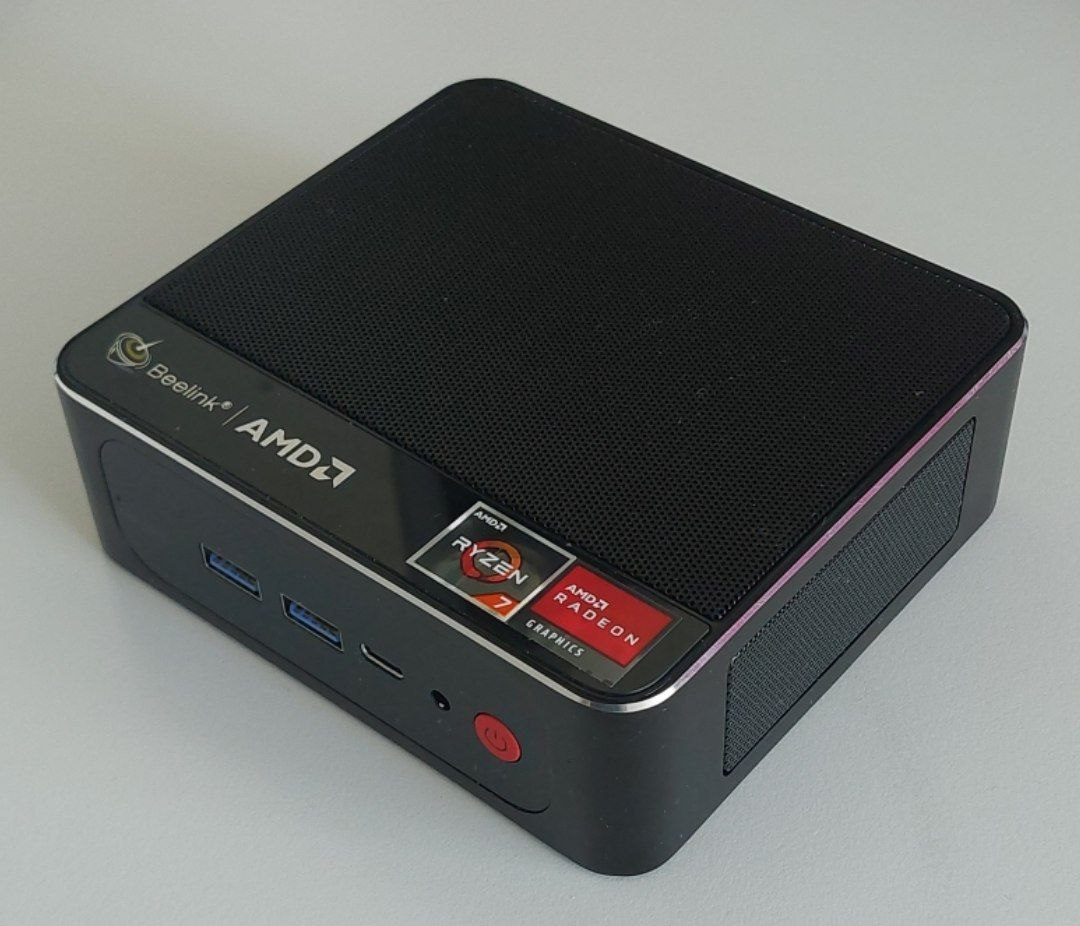
\includegraphics[width=0.4\linewidth]{img/miniPC.jpg}
	\captionof{figure}{Mini PC used}
\end{figure}\\
To improve odometry estimation, an additional sensor is integrated: the \textbf{IMU Witmotion (WIT) JY901B}. This device is a 9-Axis Combined IMU/Magnetometer/Altimeter (measure linear accelerations, angular velocities, Euler angles, magnetic field, barometry, altitude) that communicates using the TTL/UART protocol. Sensor data are acquired using the Witmotion Sensors UART Connection Library\cite{andrei_vukolov_2022_7017118}, using a USB-to-serial converter, and are published in the ROS 2 environment through a dedicated node, \texttt{witmotion\_ros}, avaible on GitHub at \\ \texttt{ElettraSciComp/witmotion\_IMU\_ros}\footnote{\href{https://github.com/ElettraSciComp/witmotion_IMU_ros/tree/ros2}{https://github.com/ElettraSciComp/witmotion\_IMU\_ros/tree/ros2}}.
\begin{figure}[h]
	\centering
	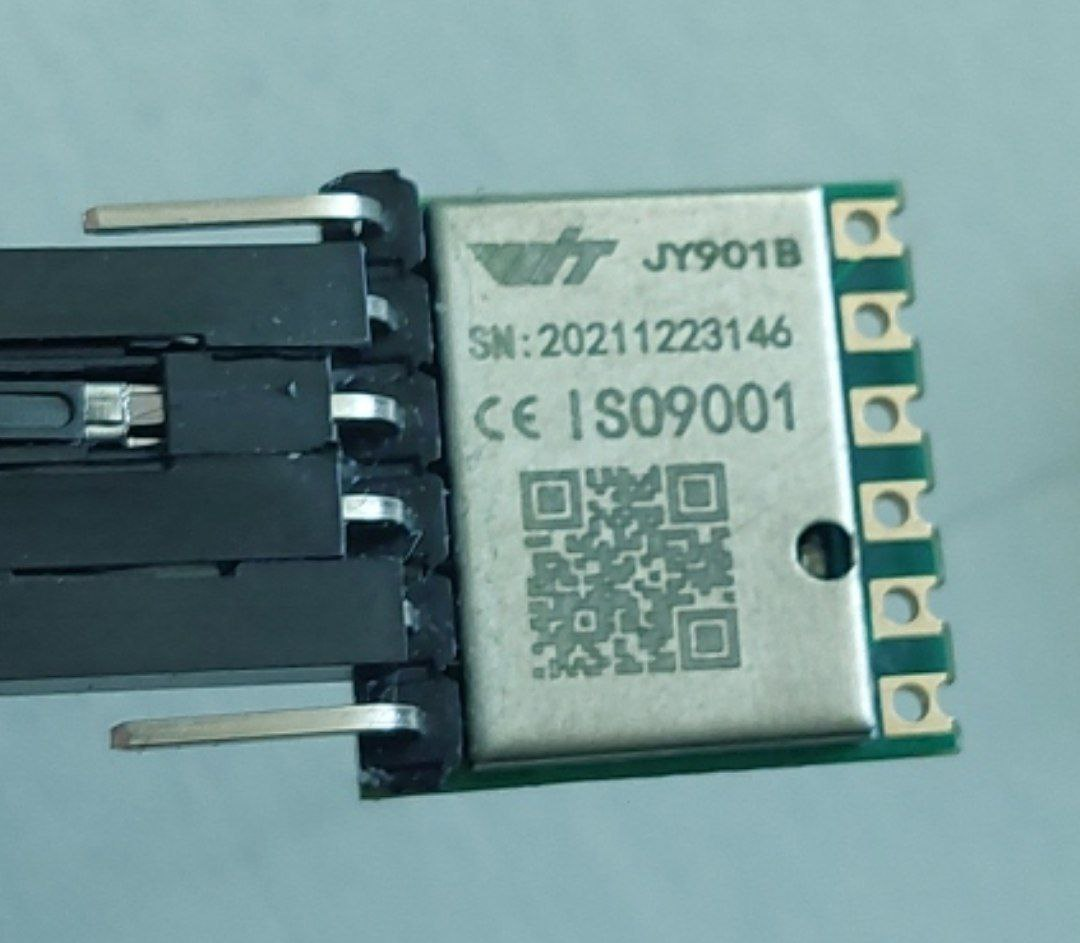
\includegraphics[width=0.4\linewidth]{img/IMU.jpg}
	\captionof{figure}{IMU used}
\end{figure}\\
For localization \ref{ref_map_to_odom}, a \textbf{2D laser scanner} is employed to provide environment perception and compensate for odometry drift by providing a transformation link between the \texttt{map} and \texttt{odom} TF frames.
The 2D laser scanner provides a cost-effective solution for environmental perception, providing dense spatial information that enables obstacle detection and basic environment recognition. Compared to alternative technologies \cite{10056144}\cite{vslamComparison2021}, it requires significantly less computational power, making it a practical choice for lightweight and resource-constrained robotic platforms.
The Laser scan used is \textbf{RPLIDAR S1} a 360 degree 2D laser scanner(LIDAR) with a distance range of 40m on white object and 10m on black ones. It features a sample rate of 9.2kHz and a scan rate ranging from 8 to 15 Hz,resulting in an angular resolution from 0.313° to 0.587°, with an accuracy of $\pm$5cm and resolution of 3cm.
The ROS 2 driver for the RPLIDAR S1 is available on Github at: \texttt{Slamtec/sllidar\_ros2}\footnote{\href{https://github.com/Slamtec/sllidar_ros2}{https://github.com/Slamtec/sllidar\_ros2}}.
\begin{figure}[h]
	\centering
	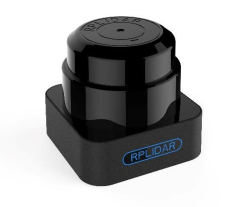
\includegraphics[width=0.4\linewidth]{img/laserScanRPLIDAR.png}
	\captionof{figure}{LIDAR used}
\end{figure}
\newpage
All components are physically mounted on the rover using custom 3D-printed parts, as shown in the following image.
\begin{figure}[h]
	\centering
	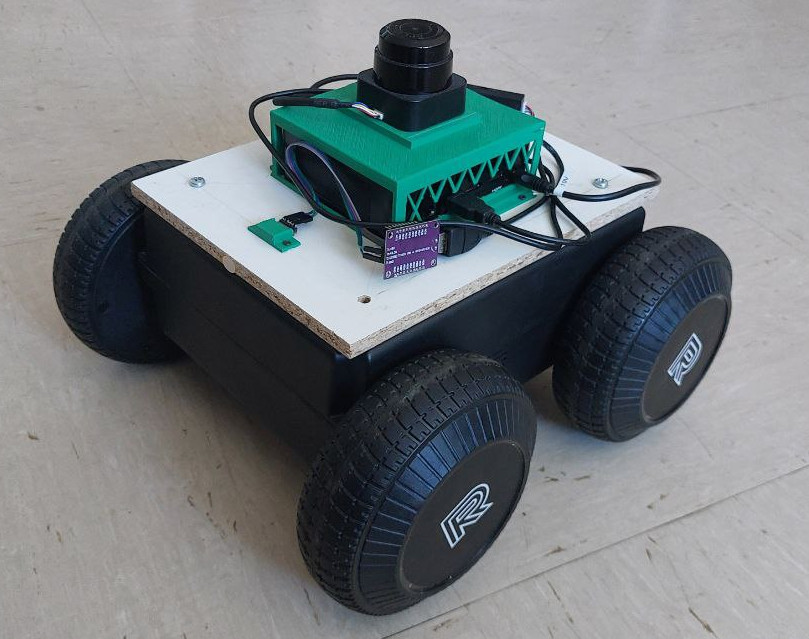
\includegraphics[width=0.4\linewidth]{img/RoverwithSensor.jpg}
	\captionof{figure}{Robot used}
\end{figure}\\
To reflect the updated hardware configuration, the original URDF (Unified Robot Description Format) file provided by the manufacturer was modified. This ensures accurate sensor placement relative to the \texttt{base\_link} frame, which is essential for proper operation of sensor-dependent ROS 2 nodes.\\
A 3D model of the robot, including all coordinate frames (TF), is shown in this picture:
\begin{figure}[h]
\centering
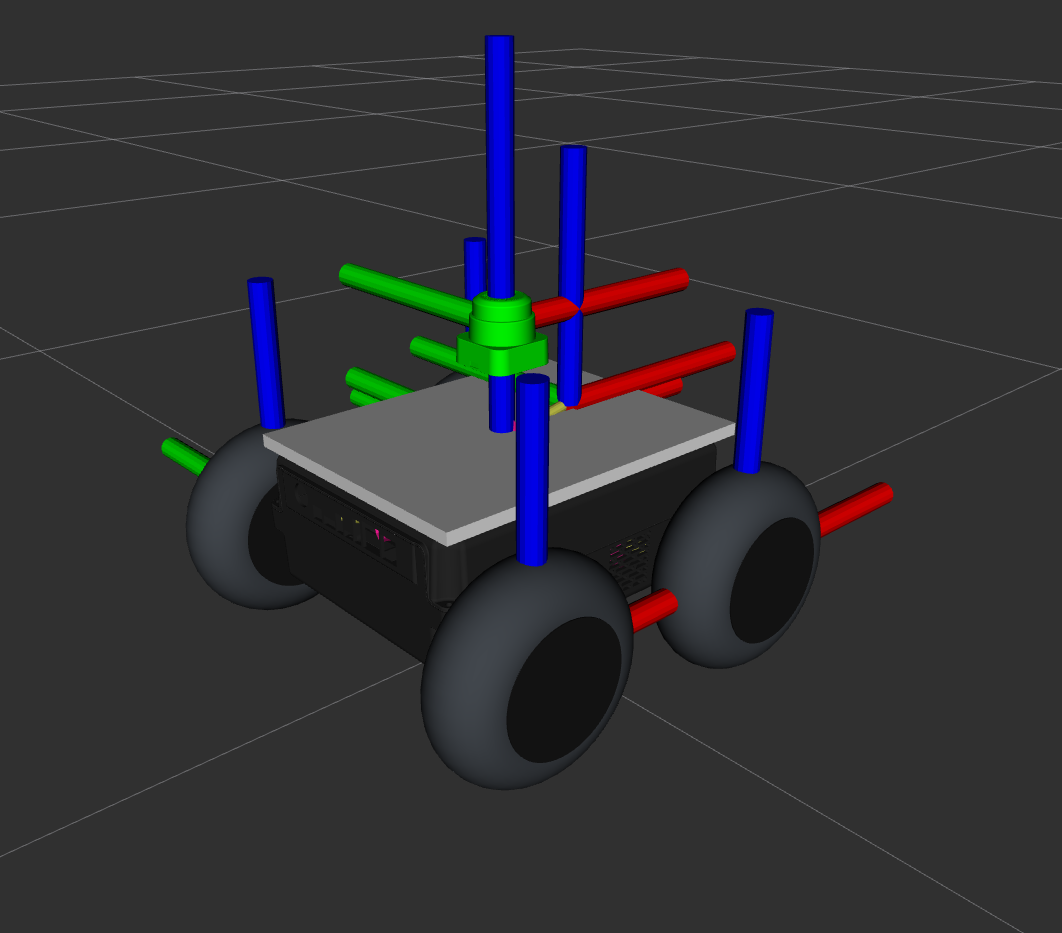
\includegraphics[width=0.4\linewidth]{img/modelWithTFtree.png}
\captionof{figure}{3D model with TF}
\end{figure}\\
With the system fully assembled, the following ROS 2 launch files are used to retrieve data from the sensors connected to the robot’s onboard mini PC:
\begin{itemize}
	\item \texttt{0.1r\_sensorLaunch.launch.py}: Launches the nodes responsible for publishing data from the IMU and LIDAR sensors.
	\item \texttt{0.2r\_mini.launch.py}: Publishes odometry data based on the built-in encoders of the robot and subscribes to the \texttt{/cmd\_vel} to move the robot.
\end{itemize}
\newpage
While, for simulation, the following launch file can be used for starting the simulation:
\begin{itemize}
	\item \texttt{0s\_ign\_mini\_gazebo.launch.py}: Launches the Gazebo simulation of the robot with all configured sensors. The \texttt{ros\_gz\_bridge/parameter\_bridge} node is used to share simulated data between Gazebo and the ROS 2 environment.
\end{itemize}
\begin{figure}[h]
	\centering
	\includegraphics[width=1\linewidth]{img/robot\_in\_simulation.png}
	\captionof{figure}{Model of the robot in Gazebo Ignition}
\end{figure}


\chapter{Steps taken to port the navigation stack from ROS 1 to ROS 2}
In this chapter, we outline the requirements for the operation of Nav2 and provide a comprehensive overview of the packages utilized by Nav2. Particular emphasis is placed on the process of porting the Global Planner module from ROS 1 to ROS 2, with a detailed discussion of the required adaptations and the challenges encountered during the transition.

\section{Odometry Estimation \texttt{odom} $\rightarrow$ \texttt{base\_link}}
As previously discussed, the raw odometry data provided by the rover are not sufficiently accurate, particularly in rotational movements\cite{MooreStouchKeneralizedEkf2014}. This is a well-known issue in odometry estimation for skid-steering vehicles, which tend to produce significant drift and errors when turning using only the data from the encoders.\\
To address this problem, the \texttt{robot\_localization} package\cite{MooreStouchKeneralizedEkf2014} was employed, specifically its \texttt{ekf\_node} Node.
This package enables the fusion of multiple sensor, even multiple instances of the same sensor type, and supports output in various ROS message formats, such as \texttt{nav\_msgs/Odometry}. It also allows preprocessing of sensor messages prior to inserting into the estimation process. The filter performs continuous state estimation and is robust to intermittent sensor data loss, maintaining a coherent position estimate over time.\\
To launch the EKF node, the following launch file was wrote:\\
\hspace*{10mm}\texttt{1<r/s>\_robot\_localizationEKF.launch.py}

\subsection{Configuration Odometry Estimation in \texttt{ekf\_node}}
As previously described and detailed in the node’s documentation\footnote{\href{https://docs.ros.org/en/noetic/api/robot_localization/html/index.html}{https://docs.ros.org/en/noetic/api/robot\_localization/html/index.html}}, we added the information about the sensors used to the configuration file. The principal information to include is the type of sensor and on which topic subscribe, \texttt{odom0:odometry/wheels} and \texttt{imu0:imu/data}, and, for each sensor, we need to choose which components of the state measurement data we want to fuse using the following array by setting the corresponding values to \texttt{true} for those we wish to include and \texttt{false} for those we do not:\\
\texttt{sensorX\_config}:$ [X, Y, Z, roll, pitch, yaw, \dot{X}, \dot{Y}, \dot{Z}, \dot{roll}, \dot{pitch}, \dot{yaw}, \ddot{X}, \ddot{Y}, \ddot{Z}] $\\
\alert{In our case, we fused the yaw angular velocity from the IMU while for the odometry we select only the velocity along the x and y in ENU (East North Up) coordinates.\\}
Additionally, the process noise covariance matrix $ Q $ can be tuned. This matrix represents the noise we add to the total error after each prediction step. Generally, the larger the value of $ Q $ relative to the variance of a given variable in an input message, the faster the filter will converge to the value indicated by the measurement.
\alert{\\
In the next section we will evaluate the performance obtained setting these parameters.
}

\subsection{\alert{Parameter changing result}}
\alert{
As describe in the paper, it allow the fusion of multiple sensor data and also expose the process noise covariance to tune it.
}
\\
\begin{figure}[h]
	\centering
	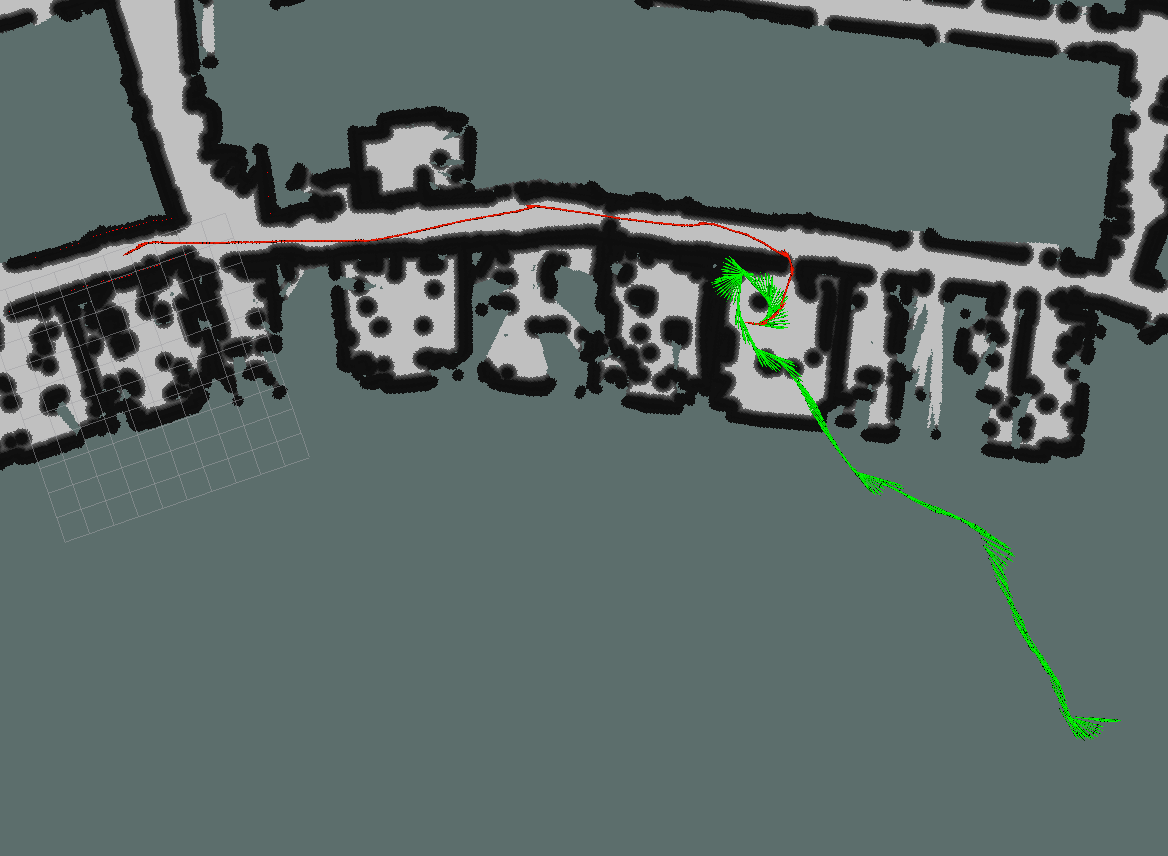
\includegraphics[width=0.9\linewidth]{img/odom_wheel_filter.png}
	\captionof{figure}{Difference in the odometry between raw data and filtered (recorded data 001)}
\end{figure}\\


\section{Localization \texttt{map} $\rightarrow$ \texttt{odom}}
In this section, we describe the process of acquiring a map and establishing the transformation between the \texttt{map} frame and \texttt{odom} frame using a localization method. This is necessary because, for long-term operation, the position of the robot in the world, using only odometry data, tends to accumulate errors and is not sufficiently accurate. Therefore, a localization technique is required to compensate for these errors\cite{sh-p1-prelude}.
\subsection{Mapping}
Although a map is already available, for completeness we provide instructions to run the following SLAM packages: \texttt{slam\_toolbox}\cite{Macenski2021} (GitHub: SteveMacenski/slam\_toolbox\footnote{\href{https://github.com/SteveMacenski/slam_toolbox/tree/ros2}{https://github.com/SteveMacenski/slam\_toolbox/tree/ros2}}) and \texttt{cartographer\_ros}\cite{45466} (GitHub: ros2/cartographer\_ros\footnote{\href{https://github.com/cartographer-project/cartographer_ros}{https://github.com/cartographer-project/cartographer\_ros}}). These packages can be launched using the following launch files:\\
\hspace*{10mm} \texttt{X<r/s>\_mappingW<slam/cartographer>.launch.py} \\
To save the generated map, use the following command, which works for both  \texttt{slam\_toolbox} and \texttt{cartographer\_ros}. This will save the map as two files:  a \texttt{.pgm} image and a \texttt{.yaml} metadata file:\\
\hspace*{10mm} \texttt{ros2 run nav2\_map\_server map\_saver\_cli -f map}\\
When using Cartographer, it is also possible to save the map as a \texttt{.pdstream} format with the following command:\\
    \hspace*{10mm} \texttt{ros2 service call /write\_state cartographer\_ros\_msgs/srv/WriteState\\ 
    \hspace*{15mm}"\{filename: "map.pdstream", include\_unfinished\_submaps :false\}"}
\newpage
\subsection{Only localization}
\remove{The map that was built using Cartographer is the following:}
\alert{The map create using Cartographer was obtained by the robot Jobot while navigating through Building T of Elettra, which serves as an office building. The map is as follows:} \\
\begin{figure}[h]
	\centering
	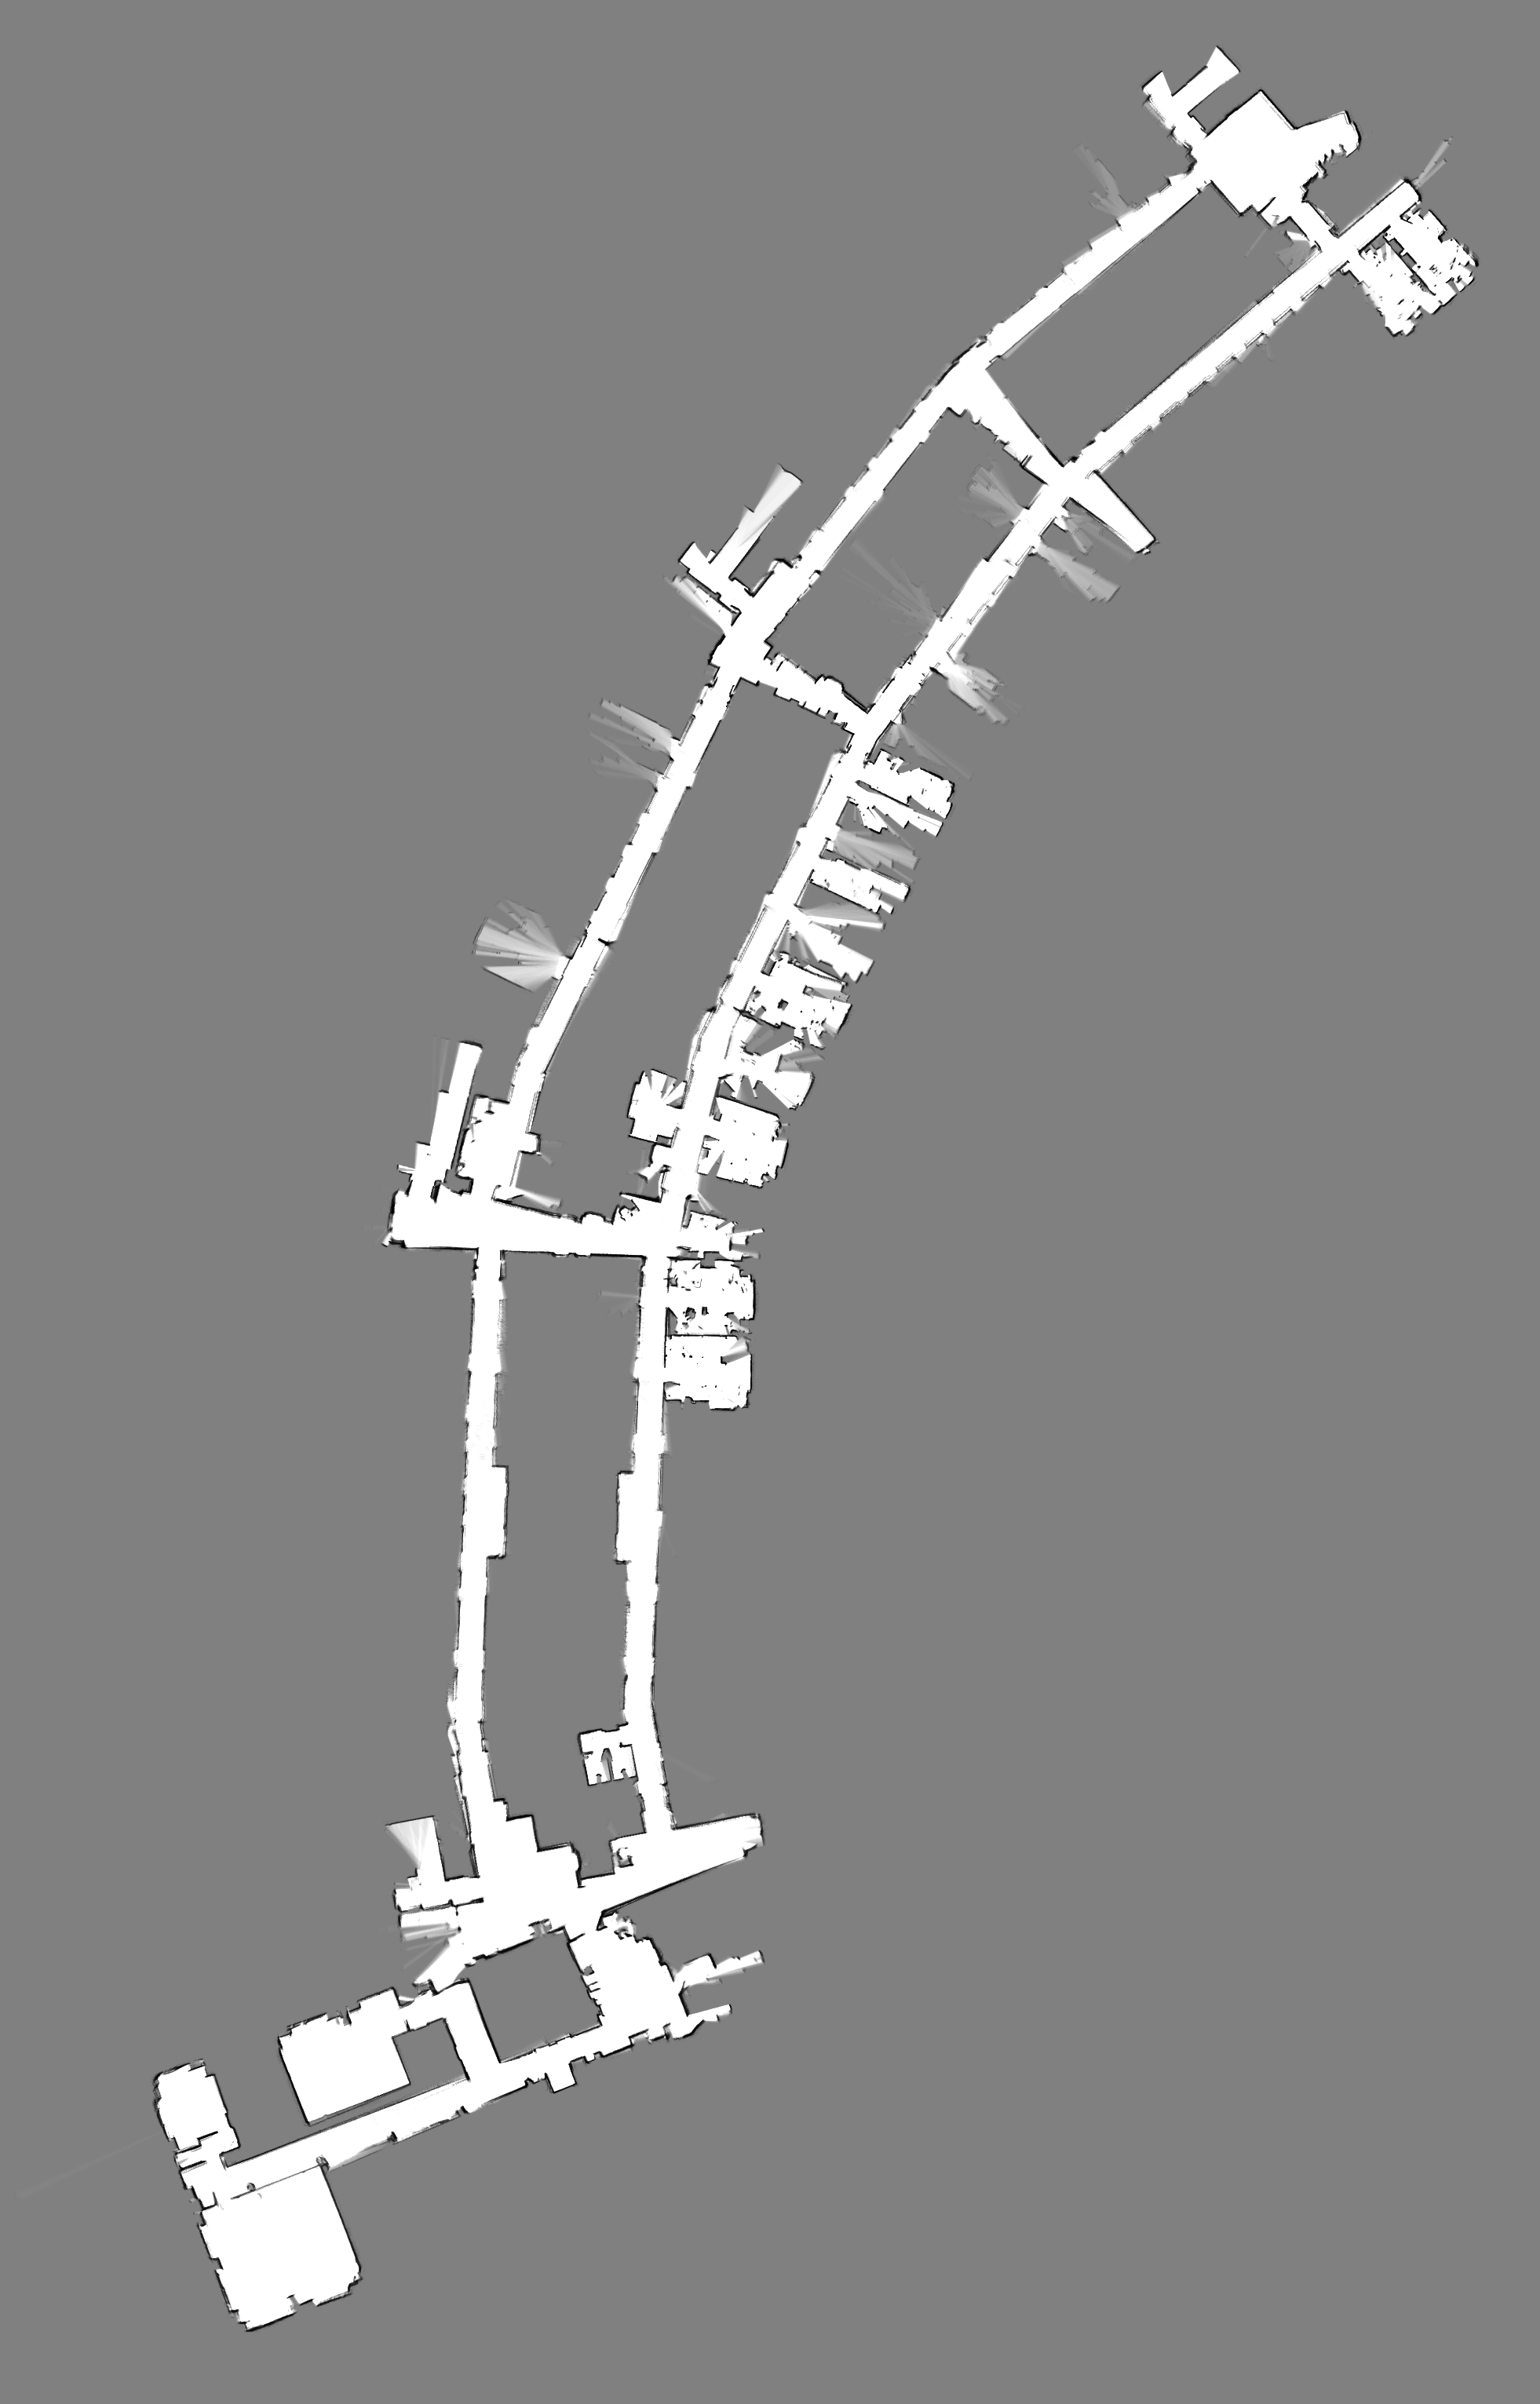
\includegraphics[width=0.4\linewidth]{img/map.png}
	\captionof{figure}{Map acquired with Cartographer}
\end{figure}\\
We initially attempted to use Cartographer solely for localization; however, due to the project’s limited maintenance, we encountered difficulties in using it effectively. As a solution, we opted for the method provided by the Nav2 package, specifically  \texttt{nav2\_amcl} and the \texttt{amcl} node.\\
One limitation of this approach is the need to convert the map acquired with Cartographer from the \texttt{.pbstream} format into a \texttt{.pgm} image and \texttt{.yaml} metadata pair, which are required by the \texttt{amcl} node. This conversion can be performed using the following command:\\
\begin{listing} [ht!]
\begin{minted}{bash} 
ros2 run cartographer_ros cartographer_pbstream_to_ros_map \
	-pbstream_filename map.pbstream \
	-map_filename map.pgm \
	-resolution 0.05
\end{minted}
\end{listing}\\
\newpage
Since certain walls in the Cartographer generated map where not solid black, due to the uncertainty of their position during mapping, the conversion process introduced errors that led to these areas to be misinterpreted as free space. As a result, the planner generated paths that passed through them. To address this issue, the walls were manually corrected using GIMP, an image editing tool, by modifying the \texttt{.pgm} map file.\\ Additionally, our planner is designed with the assumption that unknown spaces are not usable for planning. Therefore, we set the parameter \texttt{track\_unknown\_space} in the global costmap node to  \texttt{true} (\texttt{false} by default)  to achieve optimal results from our planner.
\add{aggiungere teletransport per la modifica della mappa?}
The corrected map is shown below:
\begin{figure}[h]
	\centering
	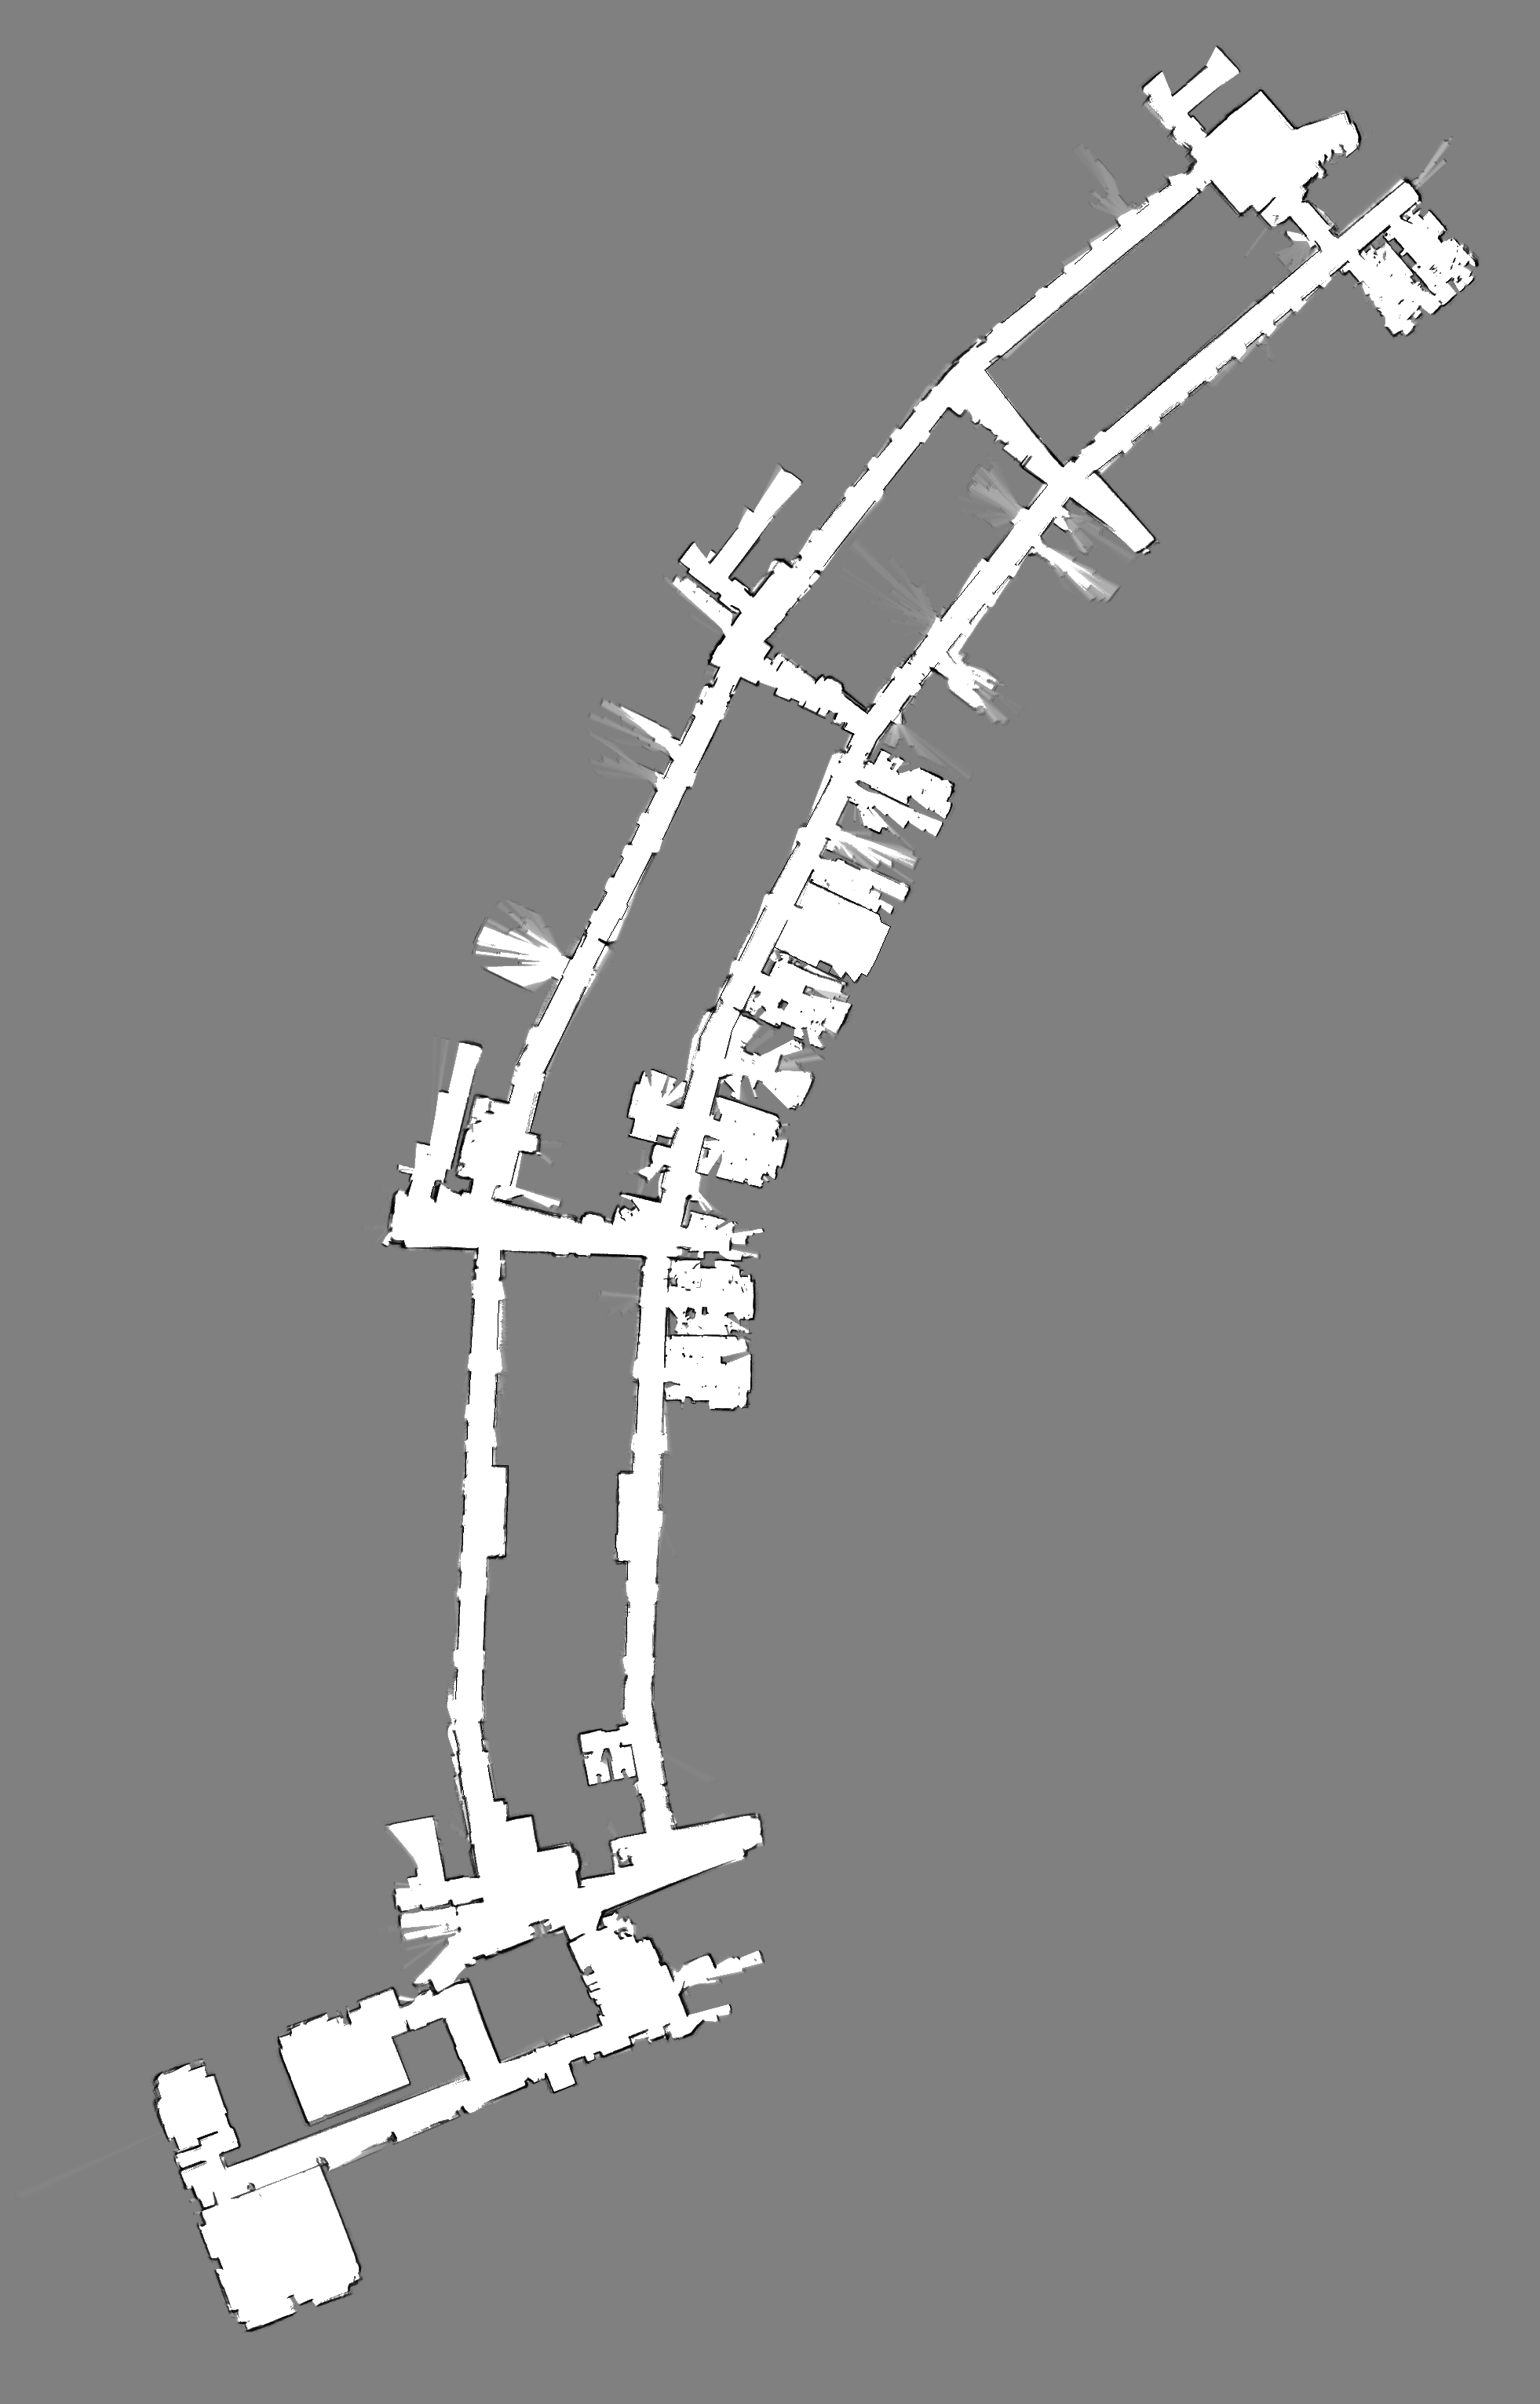
\includegraphics[width=0.4\linewidth]{img/mapV.png}
	\captionof{figure}{Map edited with Gimp and used}
\end{figure}\\
With the map properly adjusted, all necessary tools for localization are now available. We created the following launch file to initiate localization:\\
\hspace*{10mm} \texttt{3<r/s>\_L<amcl/Cartographer>.launch.py}

At this stage, all requirements are met to utilize the Nav2 navigation stack.
\section{Structure Navigation Stack Nav2}
In this section, we will discuss the components used in the Nav2 navigation stack and describe the process of porting the Global Planner from ROS 1 to ROS 2.
\subsection{Navigation Launch file}
The launch file contains all the necessary processes required for the  Navigation stack Nav2 to operate. It also implement the composition structure (\ref{Composition}) and the lifecycle manager (\ref{LifecycleNode}).
Below is a list of the core components used, along with a brief description of the plugins associated with each. Additional documentation can be found in  \footnote{\href{https://docs.nav2.org/setup_guides/algorithm/select_algorithm.html}{https://docs.nav2.org/setup\_guides/algorithm/select\_algorithm.html}} , and a migration guide is available in\footnote{\href{https://docs.nav2.org/migration/index.html}{https://docs.nav2.org/migration/index.html}} :
\begin{itemize}
	\item \texttt{nav2\_controller::ControllerServer} that use the following plugins:
	\begin{itemize}
		\item As \texttt{controller\_plugins} use \texttt{\alert{nav2\_mppi\_controller::MPPIController}}: a Model Predictive Path Integral (MPPI) algorithm to track a path with adaptive collision avoidance.
		
		\item As \texttt{progress\_checker\_plugins} use\\ \texttt{nav2\_controller::SimpleProgressChecker} that checks whether the robot has made positional progress.
		
		\item As \texttt{goal\_checker\_plugins} use \texttt{nav2\_controller::SimpleGoalChecker} that checks whether the robot has reached the goal pose.
	\end{itemize}
	
	\item \texttt{nav2\_smoother::SmootherServer} that use the following plugins:
	\begin{itemize}
		\item As \texttt{smoother\_plugins} use \texttt{nav2\_smoother::SimpleSmoother} that takes an input path and applies a lightweight smoothing algorithm. It weights the initial path points and the smoothed path points to create a balanced result where the path retains its high level characteristics but reduces oscillations or jagged features.
	\end{itemize}
	
	\item \texttt{nav2\_planner::PlannerServer} that use the following plugins:
	\begin{itemize}
		\item As \texttt{planner\_plugins} use  \texttt{dstar\_global\_planner\alert{/}DStarGlobalPlanner} that is our global planner plugin and is a implementation of the D* informed incremental search algoritm with external optimizers\cite{10.1007/978-3-031-67295-8_33}.
	\end{itemize}
	
	\item \texttt{nav2\_behaviors::BehaviorServer} that use the following plugins:
	\begin{itemize}
		\item As \texttt{behavior\_plugins} use:
		\texttt{nav2\_behaviors/Spin} performs an in-place rotation by a specified angle,
		\texttt{nav2\_behaviors/BackUp} moves the robot backward by a set distance,
		\texttt{nav2\_behaviors/Wait}  is used to pause navigation for a specified duration, allowing time for temporary occlusions to clear before resuming path planning.
	\end{itemize}
	
	\item \texttt{nav2\_bt\_navigator::BtNavigator} that use the following plugins:
	\begin{itemize}
		\item As \texttt{navigators} use\\ \texttt{nav2\_bt\_navigator::NavigateToPoseNavigator} and\\ \texttt{nav2\_bt\_navigator::NavigateThroughPosesNavigator} that utilize the default behavior trees (BT) for navigation.
	\end{itemize}
	
	\item \texttt{nav2\_lifecycle\_manager::LifecycleManager} that handling the lifecycle transition states for the stack in a deterministic way.
\end{itemize}
The simulation configuration file contains minor differences due to the use of different versions of ROS 2: Jazzy in the simulated environment and Humble on the physical robot.
In the next section, we will describe the key steps taken to port the global planner \texttt{DStarGlobalPlanner} from ROS 1 to ROS 2.
\newpage 
\subsection{Porting ROS 1 DStarGlobalPlanner to ROS 2}
As previously mentioned, the \texttt{DStarGlobalPlanner}\footnote{\href{https://github.com/ElettraSciComp/DStar-Trajectory-Planner/tree/ros2_port}{https://github.com/ElettraSciComp/DStar-Trajectory-Planner/tree/ros2\_port}} is a implementation of the D* informed incremental search algoritm with external optimizers\cite{10.1007/978-3-031-67295-8_33} for the ROS 1 \texttt{move\_base} package\footnote{\href{https://wiki.ros.org/move_base}{https://wiki.ros.org/move\_base}} 
\alert{and we want to analyze if there are some advantages of using this planner compared to the default planner.}\\
Since the code is written using ROS 1\alert{, which is not compatible with ROS 2, it will need to be ported to the newer version}. This process was divided into two main phases. In the first phase, we migrated the base structure of the package from ROS 1 to ROS 2, following these ROS 2 porting guidelines \footnote{\href{https://docs.ros.org/en/rolling/How-To-Guides/Migrating-from-ROS1.html}{https://docs.ros.org/en/rolling/How-To-Guides/Migrating-from-ROS1.html}}\footnote{\href{https://industrial-training-master.readthedocs.io/en/melodic/\_source/session7/ROS1-to-ROS2-porting.html}{https://industrial-training-master.readthedocs.io/en/melodic/\_source/session7/ROS1-to-ROS2-porting.html}}. In the second phase, we adapted the code to comply with the structure required by Nav2 planner plugins, based on the Nav2 documentation titled: "Writing a New Planner Plugin"\footnote{\href{https://docs.nav2.org/plugin_tutorials/docs/writing_new_nav2planner_plugin.html}{https://docs.nav2.org/plugin\_tutorials/docs/writing\_new\_nav2planner\_plugin.html}}.
The following subsections describe these two phases in detail. The first focuses on the structural migration to ROS 2 and the integration into the Nav2 framework. The second details the modifications needed to adapt the planner logic and interfaces to match ROS 2 conventions and the plugin architecture.
\subsubsection{Porting code from ROS 1 to ROS 2}
In the \texttt{package.xml} file, which describe the package as an organizational unit for your ROS 2 code, the following changes were made:
\begin{itemize}
	\item \texttt{buildtool\_depend} : \texttt{catking} $\rightarrow$ \texttt{ament\_cmake}: \texttt{ament\_cmake} is the new build system for CMake based packages. Compared to \texttt{catkin}, it introduces many utilities for managing packages. More information is available in the documentation\footnote{\href{https://docs.ros.org/en/rolling/Concepts/Advanced/About-Build-System.html}{https://docs.ros.org/en/rolling/Concepts/Advanced/About-Build-System.html}}.
	\item \texttt{roscpp} $\rightarrow$ \texttt{rclcpp}: \texttt{rclcpp} is the new ROS client library for C++, built on \texttt{rcl}, which provides the foundation for language-specific client libraries. \texttt{rcl} communicates with \texttt{rmw}(ROS middleware interface), which handles the communication with \texttt{DDS} (Data Distribution Service).
	\item Updated package naming to follow the ROS 2 conventions.
	\item To inform \texttt{colcon} that the package uses \texttt{ament\_cmake}, the build type must be explicitly specified in the \texttt{build\_type}.
\end{itemize}
Subsequently, the \texttt{CMakeLists.txt} file was updated with the following major changes:
\begin{itemize}
	\item Package names were updated to reflect ROS 2 naming conventions.
	\item C++ standard was set to 17.
	\item \texttt{find\_package()} is required to be called for each package.
	\item \texttt{ament\_export\_dependencies()}  is used to declare runtime dependencies.
	\item The package must be declared in ROS with \texttt{ament\_package()}.
\end{itemize}
Other minor changes are:

\begin{itemize}
	\item Log calls were updated from \texttt{ROS\_} to \texttt{RCLCPP\_}
	\item Message type structures changed (e.g.,\\ \texttt{geometry\_msgs::PoseStamped} $\rightarrow$ \texttt{geometry\_msgs::msg::PoseStamped}).
	\item The structure of the C++ program now required the use of smart pointer.
\end{itemize}

Additional changes specific to the ROS 2 Navigation stack Nav2 are discussed in the following section.

\subsubsection{Porting code from ROS 1 Navigation stack to Nav2}
The following changes were made to port the planner to the Nav2 framework:
\begin{itemize}
	\item Since the planner is a \textbf{global planner}, it now inherits from the new abstract interface \texttt{nav2\_core::GlobalPlanner}. As a result, we updated the\\ \texttt{global\_planner\_plugin.xml} file to change the \texttt{base\_class\_type} accordingly.
	\item As a plugin based on \texttt{nav2\_core::GlobalPlanner}, the planner must implement five pure virtual methods required for proper operation: \texttt{configure()}, \texttt{activate()}, \texttt{deactivate()} and \texttt{cleanup()}, \texttt{createPlan()}. Below is a description of each method:
	\begin{itemize}
		\item \texttt{configure()}: it's called when the node enters \texttt{on\_configure} state. This method is responsible for declaring ROS parameters and initializing the planner's member variables. It takes the following input parameters:
		\begin{itemize}
			\item \texttt{rclcpp\_lifecycle::LifecycleNode::WeakPtr}  A weak pointer to the base lifecycle node.
			\item The planner’s name as a \texttt{std::string}.
			\item A share pointer to the \texttt{tf} buffer\\ \texttt{std::shared\_ptr<tf2\_ros::Buffer>}.
			\item A shared pointer to the costmap\\ \texttt{std::shared\_ptr<nav2\_costmap\_2d::Costmap2DROS>}.
			\item For jazzy also: \texttt{std::function<bool()> cancel\_checker} that allow for the cancellation of the current planning task.
		\end{itemize}
		This replace the \texttt{initialize} method and the class initialization used in ROS 1.
		\item \texttt{activate()}: Called when the node enters \texttt{on\_activate} state, used for implement operations which are necessary before planner goes to an active state. In our case, we allocate memory and fill our internal costmap \texttt{state\_map}, which is used by the D* (\texttt{dstar}) algorithm.
		\item \texttt{deactivate()}: Called when the node enters \texttt{on\_deactivate} state. This method is used for implementing operations which are necessary before planner goes to an inactive state. In our case, this method is not used and is left empty.
		\item \texttt{cleanup()}: Called when the node enters \texttt{on\_cleanup} state. This method is used for cleaning up resources which are created for the planner. In our case we destroys the allocated memory used by \texttt{state\_map} and \texttt{dstar}. 
		\item \texttt{createPlan()}: Invoked when the planner server requests a global plan between a start and goal pose. It required the start and goal position as\\ \texttt{geometry\_msgs::msg::PoseStamped} and return a path \texttt{nav\_msgs::msg::Path}. It replace the \texttt{makePlan} used in ROS 1.
	\end{itemize}
	\item At the end of the C++ code,  we added the following lines to export the planner as a plugin:\\
\begin{listing} [ht!]
\begin{minted}{cpp} 
#include "pluginlib/class_list_macros.hpp"
PLUGINLIB_EXPORT_CLASS(<type of the plugin class>, <type of the base class>);
\end{minted}
\end{listing}
	\item Because it is a plugin,it is necessary to provide a description using a plugin declaration file. This is done by creating a file named \texttt{global\_planner\_plugin.xml} in the same directory as the \texttt{package.xml}.
	The \texttt{global\_planner\_plugin.xml} file specifies the plugin's class type and the base class it inherits from, following the format required by the pluginlib system. Then we edit the CMake file as described in the documentation\footnote{\href{https://docs.ros.org/en/rolling/Tutorials/Beginner-Client-Libraries/Pluginlib.html}{https://docs.ros.org/en/rolling/Tutorials/Beginner-Client-Libraries/Pluginlib.html}}.
\end{itemize}
\subsubsection{Building the project}
The system was built using the new build tool, \texttt{colcon}\footnote{\href{https://github.com/colcon}{https://github.com/colcon}}. It is a command line tool to improve the workflow of building, testing and using multiple software packages. It automates the process, handles the ordering and sets up the environment to use the packages.\\
After successful compilation, the global planner is ready for use within the Nav2 framework.

\chapter{Jobot porting procedure to ROS 2}


Elettra has also a Jobot, a 2WD rover still based on ROS 1, it was decided to port it to ROS 2 in order to effectively evaluate the use of Open-RMF.
\section{Jobot Description}
Jobot is a 6-wheeled rover with a 2WD configuration. It is equipped with a mini PC that collects data from an RPLIDAR A2 laser sensor and acceleration data from a serial bus connected to an Arduino microprocessor, which is linked to an IMU. An image of the robot is available in \ref{fig:Jobot Rover}:\\
The steps taken to port the code in ROS 2 are described in the following section.

\section{What changes where made in the code}

The code use the serial ROS 1 library to communicate to the Arduino and retrieve the data from the encoders and the IMU. This library is no longer available in ROS 2, so to avoid rewriting the structure of the Jobot code, we utilized the same library that has been ported to ROS 2, which is available on GitHub: 
https://github.com/iwelch82/serial-ros2.git .
The retrieved data is used to publish the odometry pose estimation of the robot, while a secondary node handles the IMU data.\\
The secondary node for publishing the IMU data was updated to ROS 2 by simply using the base node logic, whereas the main node was rewritten using the lifecycle structure. This logic is employed to configure the node during the on\_configure method, and if it fails or a request for deactivation or cleanup is made, it stops and cleans everything. This structure allow to remotely control the passage through the states, for now and in our case it will be connected to an automatic Node manager used in nav2, the \texttt{lifecycle\_manager} in \texttt{nav2\_lifecycle\_manager}. This node check all the states of the nodes that are connected to it and sequentially configures and activates them. If a crash occurs or if we stop a specific node's process, the lifecycle communicates the change of state and activates a procedure to stop the connected nodes. This node is only called in the launch file.\\
In addiction we updates the custom messages to ROS 2 that the Jobot use internally.\\
Once everything is configured, the node starts to publish the robot's state odometry but does not publish static transforms between the sensors. These transforms are manually published using the \texttt{static\_transform\_publisher} provided by \texttt{tf2\_ros}.\\

To minimize changes, the software is built inside a Docker container, and all applications are launched from it.\\

This, along with the same software used for navigation, enables this platform to function as an autonomous mobile robot (AMR).\\


\newpage
\section{Create a model for the simulation}

For simulation purpose, we need to create a model  of the Jobot in the URDF format, which will be used by Gazebo to build a 3D representation and generate data from the sensors equipped on it.\\
Since Jobot has a 2WD configuration, we will add two cylinders as wheels, which will be controlled by the Gazebo plugin \texttt{ignition::gazebo::systems::DiffDrive}. This plugin allows the robot to receive velocity commands and move accordingly.\\
Next, we add the sensors gazebo type\texttt{IMU} and \texttt{gpu\_lidar} to simulate the IMU and the lidar on the robot. This procedure is similar to the one used for the Mini Rover from the Rover Robotics.
At the end we obtain the following model:

\begin{figure}[h]
	\centering
	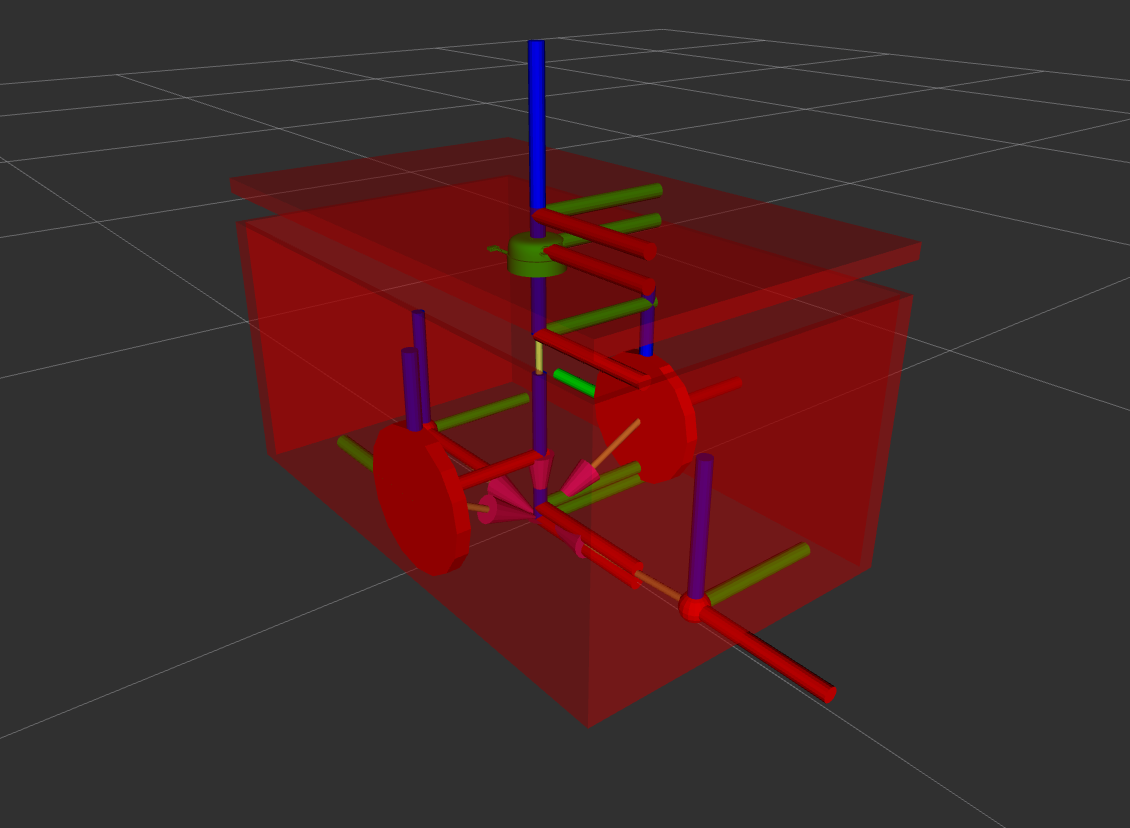
\includegraphics[width=0.6\linewidth]{img/jobot_tf_strucure.png}
	\captionof{figure}{Jobot robot URDF model}
\end{figure}


\chapter{Integration of the navigation stack with Open-RMF}
To integrate a fleet in Open-RMF, we first need information about the building's infrastructure, such as automatic doors or lifts that can be controlled, and the \textbf{route maps} that robots can use. \textbf{Route maps} are essential for predicting the paths robots will take, enabling Open-RMF to perform effective \textbf{traffic management} and avoid conflicts. All these information have to be stored in a file that can be generated using the \textbf{traffic editor tool}\footnote{\href{https://github.com/open-rmf/rmf\_traffic\_editor}{https://github.com/open-rmf/rmf\_traffic\_editor}}  \footnote{\href{https://osrf.github.io/ros2multirobotbook/intro.html}{https://osrf.github.io/ros2multirobotbook/intro.html}}, a tool provided by Open-RMF. The following section describes how the Traffic Editor works and how we used it in our implementation.
\section{Traffic Management - Route Maps Generation}
To begin describing the environment for Open-RMF, we created a new project in the Traffic Editor by generating a \texttt{.building.yaml} file. We then imported both the map produced by Cartographer and the floor plan of the facility.After importing the map,we defined the positions of key elements and planned the traffic flow for the floor, following best practices as outlined in the Open-RMF documentation\footnote{\href{https://osrf.github.io/ros2multirobotbook/integration\_nav-maps-strategies.html}{https://osrf.github.io/ros2multirobotbook/integration\_nav-maps-strategies.html}}. The following components of the Traffic Editor were used to encode the necessary environment data:
\begin{itemize}
	\item \textbf{vertex}: They are waypoints or a part of the description of walls, doors or else. Each vertex can have several properties:
	\begin{itemize}
		\item \texttt{is\_holding\_point} : Indicates that the robot is allowed to wait at this waypoint for an indefinite period of time.
		\item \texttt{is\_parking\_spot}: Designates a parking location for a robot.
		\item \texttt{is\_passthrough\_point}: A waypoint where the robot should not stop.
		\item \texttt{is\_charger}: Identifies a charging station.
		\item \texttt{is\_cleaning\_zone}: Used to indicate that this waypoint belong to a cleaning zone for the \texttt{Clean} task.
		\item \texttt{dock\_name}: Used for triggering docking behavior via RMF.
		\item \texttt{pickup\_dispenser}: Specifies a dispenser workcell for \texttt{Delivery} tasks.
		\item \texttt{dropoff\_ingestor}: Specifies an ingestor workcell for \texttt{Delivery} tasks.
		\item \texttt{spawn\_robot\_type}: Used in simulation to spawn a robot model.
		\item \texttt{spawn\_robot\_name}: Used in simulation to identify a spawned robot.
	\end{itemize}
	\item \texttt{measurement}: Connects two vertex and is used to set the scale of the drawing. In our case, we used the width of a door.
	\item \texttt{door}: Connects two vertex and is used for interacting with the real world and simulate doors. If a robot encounters a door on its route, RMF sends a command to open it. When generating the simulation world model, a controllable door model is automatically added.
	\item \texttt{traffic lane}: Connects two waypoints and define the paths that fleets will follow. Lanes can be grouped, assigned to specific fleets, and configured as unidirectional or bidirectional. An optional "orientation" setting can be specified to require robots to move forward or backward along the lane. During planning, Open-RMF assumes that all traffic lanes are straight lines.
	\item \texttt{fiducials}: Used for multi-floor alignment and as anchors for the ROS 2 map. They provide spatial reference points between floors.
	\item \texttt{lift}: Is used for interacting with the real world and simulate elevators. If a robot goes to a lift, RMF sends a command to call it and, when the robot reach the waypoint, it send the lift to the designed floor. When generating the simulation world model, a controllable lift model is automatically added.
	\item \texttt{walls}: Connect two waypoints to define the location of a wall in the environment. When generating the simulation world, a wall is created between these points.
	\item \texttt{floor}:  Add the ground plane for robots in the simulation world. This component can be modified to include holes (e.g., for elevator shafts).
	\item \texttt{environment assets}: Adds Gazebo models of various furniture and objects to the simulation, helping to create a realistic environment for testing and validation.
\end{itemize}
In the process of designing route maps, several strategic choices were made:
\begin{itemize}
	\item Only one robot is allowed in a hallway at a time.
	\item Holding points (leaf nodes) were added along corridors or near their entrances and exits to allow one robot to yield to another already in the hallway. For certain task-specific waypoints, it is recommended to assign a very low speed limit to discourage RMF from using them as generic holding points.
	\item Mutex groups were defined on lanes and waypoints to ensure exclusive access, avoiding deadlocks by allowing only one robot to occupy a mutex-assigned group at any time.
\end{itemize}
\newpage
At the end we obtained the following configuration map:\\
\begin{figure}[h]
\centering
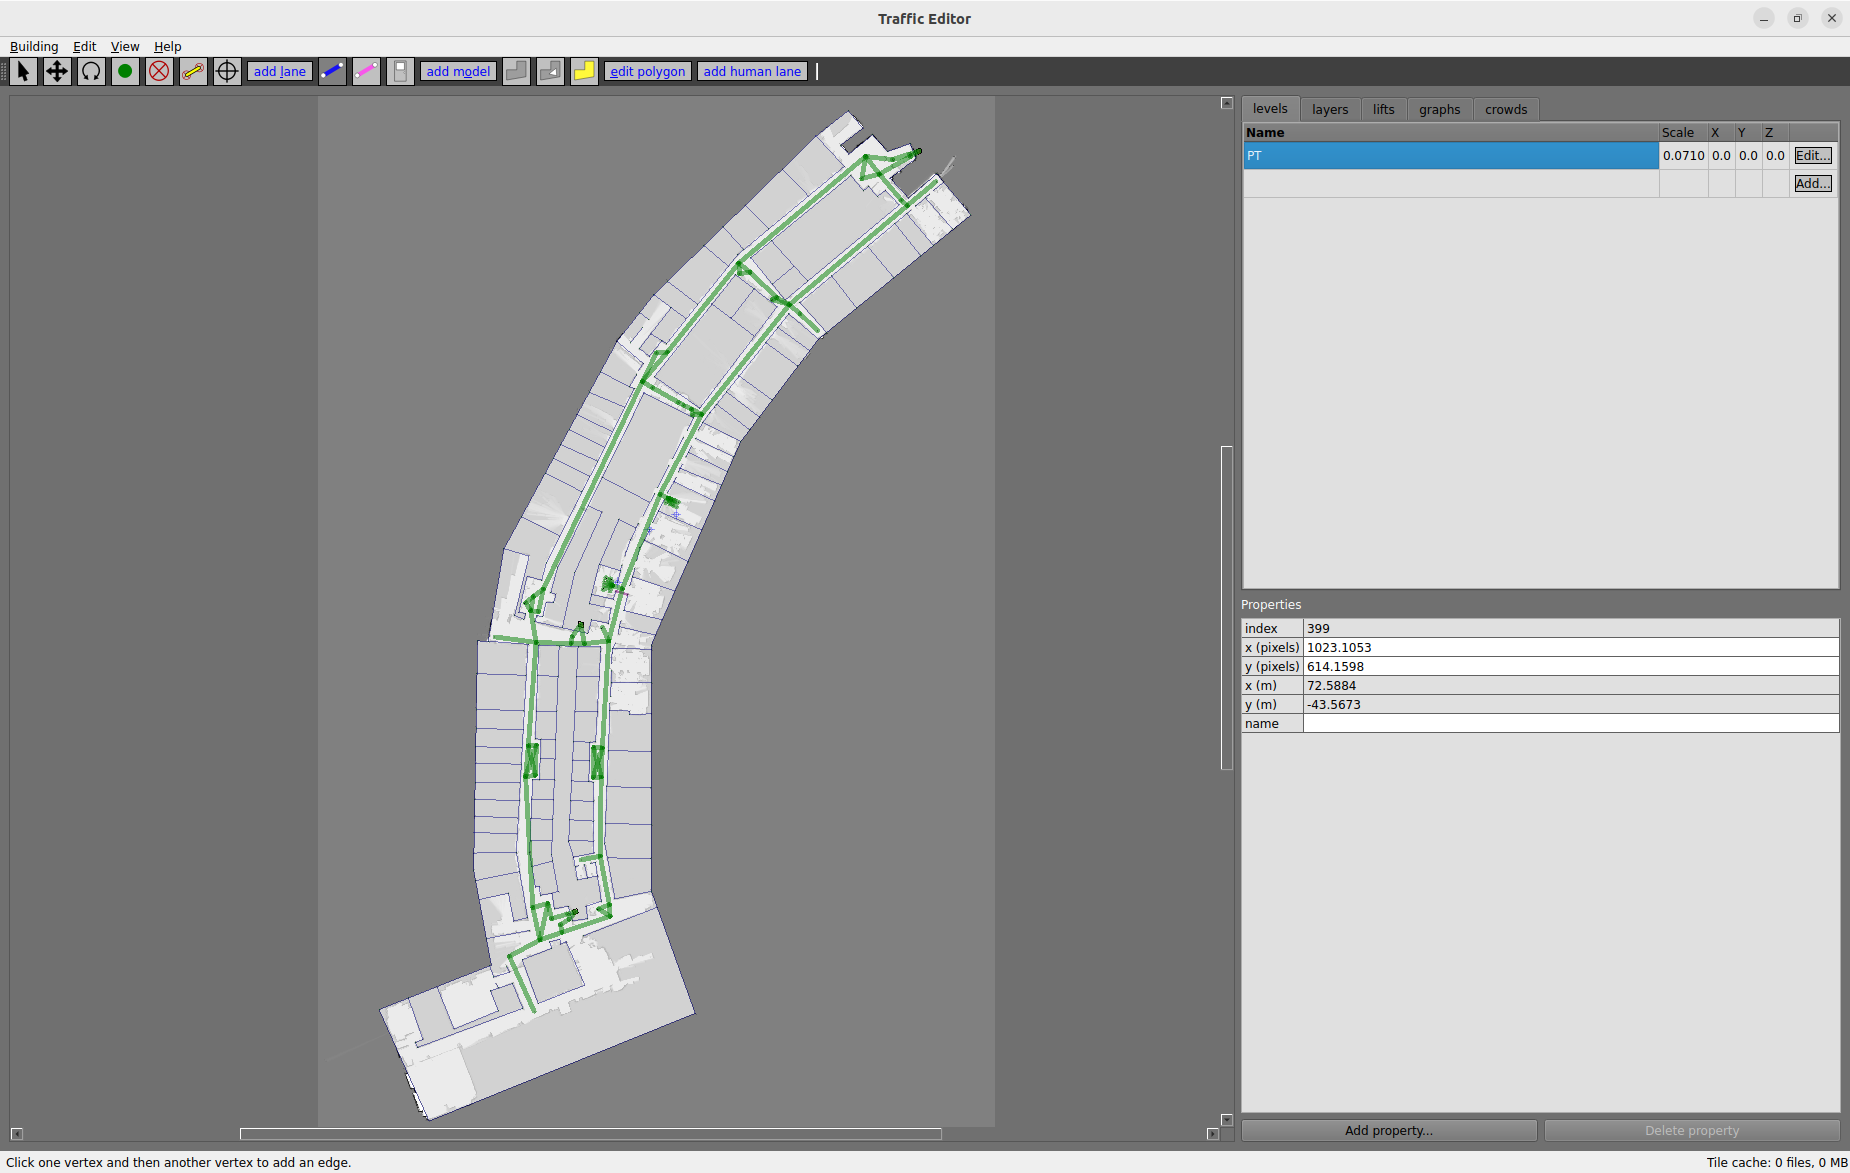
\includegraphics[width=1\linewidth]{img/RMF-traffic-map.png}
\captionof{figure}{Traffic editor with Elettra's route map}
\end{figure}\\
The route map \texttt{.yaml} files for each graph can be generated using the following command:\\
\texttt{ros2 run rmf\_building\_map\_tools building\_map\_generator nav \textbackslash \\ \hspace*{1cm} \$\{building\_map\_path\} \$\{output\_nav\_graphs\_dir\}}\\
\vspace*{5mm}\\
For the simulation, the world can be generated using the following command:\\
\texttt{ros2 run rmf\_building\_map\_tools building\_map\_generator ignition \textbackslash{}\\ \hspace*{1cm}
\$\{building\_map\_path\} \$\{output\_world\_path\} \$\{output\_model\_dir\}}\\
And the following command can be used to download the models required for the simulation world:\\
\texttt{ros2 run rmf\_building\_map\_tools building\_map\_model\_downloader \textbackslash{} \\ \hspace*{1cm}
\$\{building\_map\_path\} -f -e \mytexttilde/.gazebo/models}\\

\newpage
The simulation environment generated from the configuration resulted in the following world:\\
\begin{figure}[h]
	\centering
	\includegraphics[width=1\linewidth]{img/rmf\_generated\_world.png}
	\captionof{figure}{World generated using traffic editor}
\end{figure}\\

We can now launch the core components of RMF.

\section{RMF core}
This is the launch file used to start the core components of RMF:\\
\texttt{0\_rmf\_core.launch.xml}\\

This launch file starts the following nodes, which form the core structure of RMF:
\begin{itemize}
	\item \texttt{rmf\_traffic\_schedule} : Manages traffic scheduling by controlling path structures, publishing itinerary topics, and handling conflict resolution.
	\item \texttt{rmf\_traffic\_blockade} : Acts as the Traffic Blockade Moderator, managing checkpoint information.
	\item \texttt{building\_map\_server} : Publishes map data, including points of interest such as parking spots.
	\item \texttt{visualization.launch.xml}: Optional nodes that launches visualization tools for monitoring and controlling RMF via rviz2.
	\item \texttt{door\_supervisor}: Publishes control requests for doors using ROS communication structures.
	\item \texttt{lift\_supervisor}: Publishes control requests for lifts using ROS communication structures.
	\item \texttt{rmf\_task\_dispatcher}: Allow to dispatch submitted task to the best fleet/robot within RMF.
	\item \texttt{queue\_manager}: Manages reservations for parking spots and helps prevent conflicts.
\end{itemize}

Once the core system is launched, the next step is to connect our fleets using \textbf{fleet adapters}. Open-RMF provides the Free Fleet adapter, which is compatible with ROS 2 and Nav2. The following section will detail how this adapter works and how we integrated it into our system.

\section{Free Fleet}
Free fleet\footnote{\href{https://github.com/open-rmf/free\_fleet}{https://github.com/open-rmf/free\_fleet}} is a python implementation of the \texttt{full\_control} Open-RMF Fleet Adapter\footnote{\href{https://github.com/open-rmf/fleet_adapter_template}{https://github.com/open-rmf/fleet\_adapter\_template}}, which serves as a general template for communicating with a fleet manager. Its primary goal is to control robots running under both ROS 1 and ROS 2.
It uses \texttt{zenoh} as a communication layer between each robot and the fleet adapter.
Below is an overview of how communication is managed using the Free Fleet adapter:
\begin{figure}[h]
	\centering
	\includegraphics[width=1\linewidth]{img/free\_fleet\_adapter.png}
	\captionof{figure}{Free Fleet Adapter Communication}
\end{figure}
\subsection{Setup fleet}
To use the Free Fleet, it is necessary to create a \texttt{.yaml} configuration file for the fleet. This file describes the robots within the fleet that share the same characteristics. The configuration includes essential information such as the fleet name, velocity limit of the fleet, robot dimensions and mechanical details, power management parameters, the tasks the fleet are capable of performing, a list of all robots in the fleet with their individual names and their assigned chargers. It also need the positional correlation between the robot’s map and the RMF map.\\
After setting up the fleet configuration, the next step is to configure Zenoh for communication.
\subsection{Setup Zenoh}
Zenoh\footnote{\href{https://zenoh.io/}{https://zenoh.io/}} is a pub/sub/query protocol that unifies data in motion, data at rest and computations. It combines traditional pub/sub with geo distributed storage, queries and computations, while maintaining high efficiency in both time and space. Zenoh allows selective topic transmission over the network, reducing bandwidth usage to specific servers.\\
To set up Zenoh for use with Free Fleet, the following steps are required:
\begin{itemize}
	\item Zenoh router must be running on a server. This router can be launched using the command: (\texttt{\$ zenohd}). Multiple instances of the Zenoh router can be run for redundancy.
	\item On each robot and on the RMF server, the standalone executable\\ \texttt{zenoh-bridge-ros2dds} must be launched with the associated configuration file. This executable bridges all ROS 2 communications using DDS over Zenoh. The configuration of this file depend on the machine. On the server it's configured to accept all the traffic from each robot, while on the robot we need to setup:
		\begin{itemize}
		 \item The \texttt{namespace}, which must match the fleet configuration file namespace.
		 \item Enabling the publication of the robot’s frame status topics (\texttt{.*/tf} and \texttt{.*/tf\_static}) and battery information (\texttt{.*/battery\_state})
		 \item Enabling communication with action servers controlling navigation\\ (\texttt{.*/navigate\_to\_pose})
		 \item Zenoh-specific configuration details, such as the communication mode, the server address, the protocol and the port for connection endpoints (e.g., \texttt{tcp/<ip address server>:7447})
		\end{itemize}
\end{itemize}
\subsection{Launching Free Fleet}
After completing the setup, we can use the following launch file to start the Free Fleet adapter:\\
\texttt{1rmf\_mini\_fleet\_adapter.launch.xml}\\
This launch file takes as parameters the fleet configuration file and the route maps that the fleet will use. Once launched, it is possible to monitor the robot topics on the RMF server.
\\Also this is replicated for the Jobot fleet, launching the following file\\
\texttt{1rmf\_jobot\_fleet\_adapter.launch.xml}\\

\newpage
\section{Web interfaces}
Open-RMF also offers a web-based interface, \texttt{rmf-web}\footnote{\href{https://github.com/open-rmf/rmf-web}{https://github.com/open-rmf/rmf-web}}, to visualize and control the system on a browser. It consists of two main components:
\begin{itemize}
	\item api server : Based on the OpenAPI specification and implemented with the Python FastAPI library, it provides REST API methods to communicate with Open-RMF.
	\item dashboard :  In our case, a demo dashboard that connects to the API server and allows control of the fleet.
\end{itemize}

Both components are available as Docker images and can be launched with the command:\\
\texttt{docker compose -f /path/to/compose.yml up}

Then we can connect to the web dashboard:
\begin{figure}[h]
	\centering
	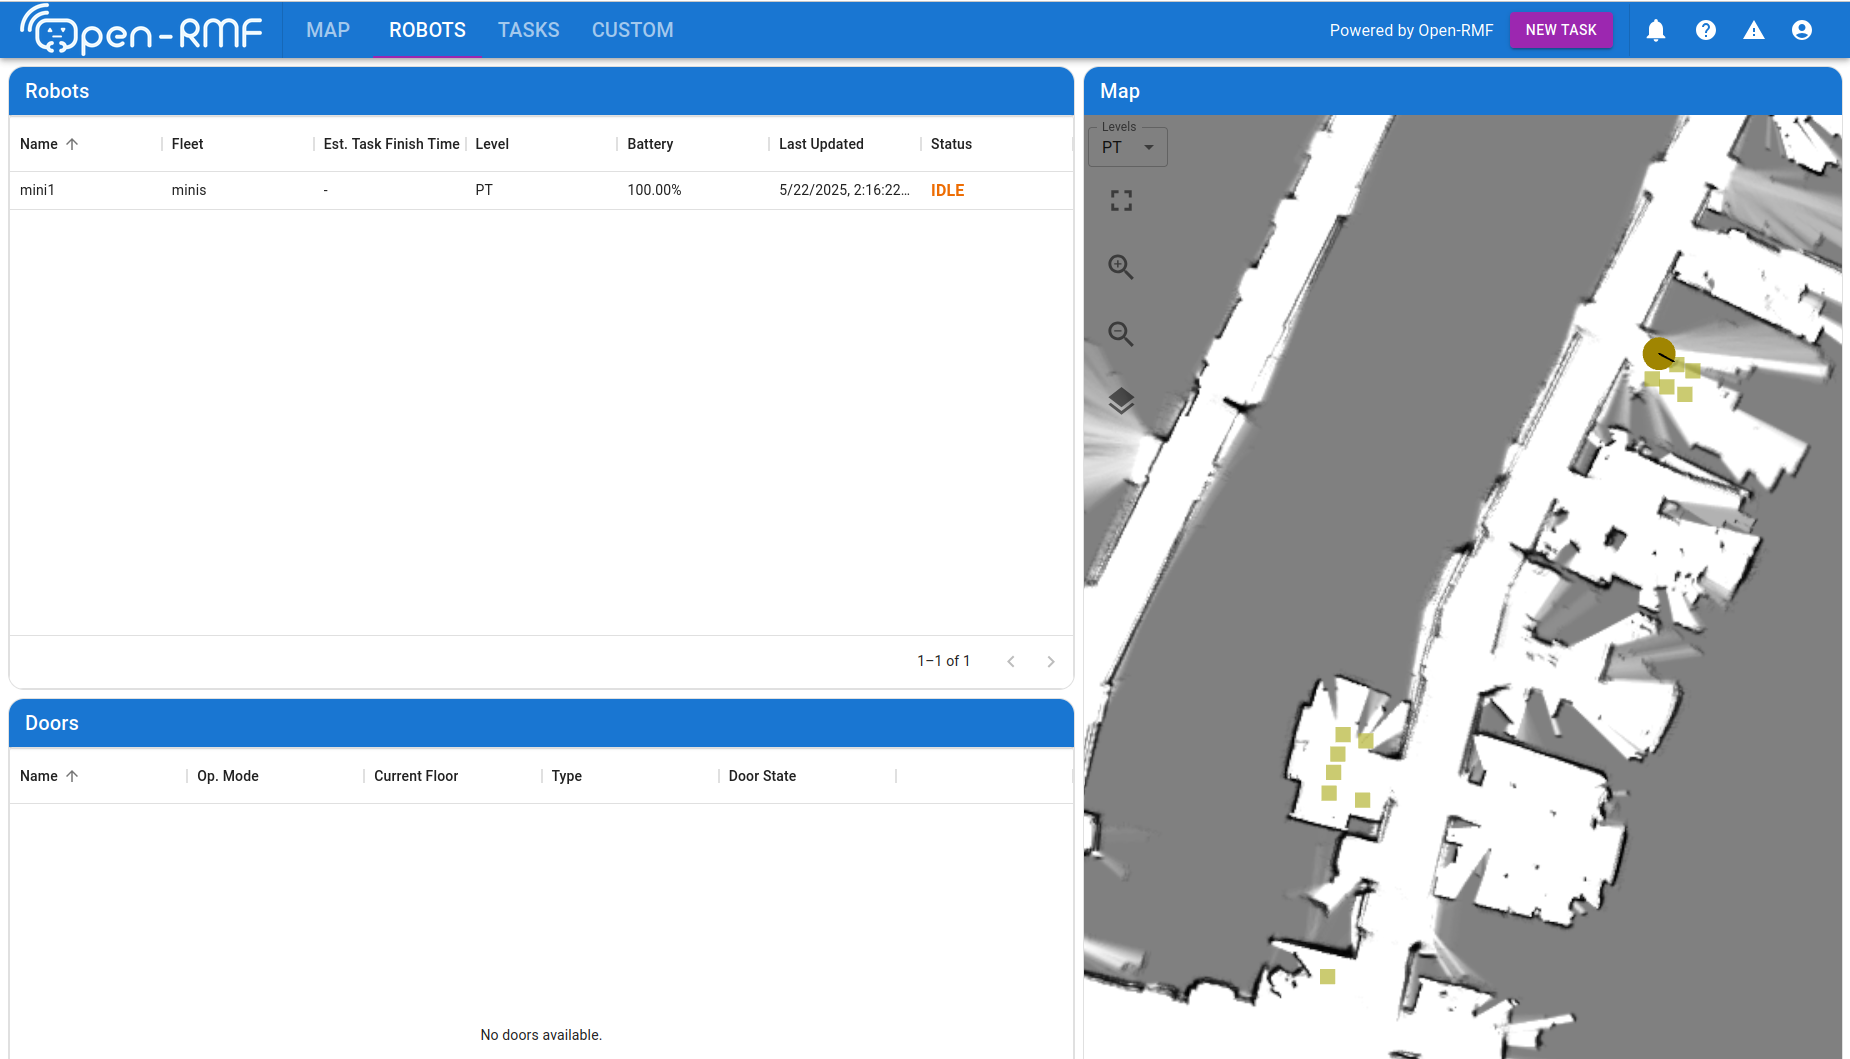
\includegraphics[width=1\linewidth]{img/openRMF-dashboard.png}
	\captionof{figure}{Open-RMF Web Dashboard}
\end{figure}

\chapter{\alert{Testing and evaluation of the system}}
After some testing, these are the problems we found:
\begin{itemize}
\item The testing revealed some design issues with the rover. 
When operating in an office environment, the robot’s laser sensor cannot detect certain parts of obstacles, as shown in the image below.
\begin{figure}[h]
	\centering
	\includegraphics[width=1\linewidth]{img/problem\_chair.jpg}
	\captionof{figure}{Laser position error}
\end{figure}\\
One possible solution is to reduce the free space from the occupancy map. However, the dimensions of the chair legs are quite long, significantly reducing the available space to pass through doors, which the planner currently prevents.
Another option is to relocate the LIDAR sensor underneath the robot. This would require a low-profile LIDAR and would create blind spots by the wheels if no additional sensors are added on top.
Alternatively, adding a depth camera could provide a 3D occupancy grid, which can then be processed to generate a simpler 2D map.
 
\item The RMF commands from waypoint to waypoint: RMF commands the robot from waypoint to waypoint, and it leaves the low level navigation to each robot's navigation stack. So if the robot chooses to use a non-straight route, it means that the RMF navigation graph might need to be re-drawn or reconsidered (if there are constant obstacles around), or the navigation stack of the robot should be tuned to allow tighter tolerances for static/dynamic obstacles. but how the robot chooses to navigate between them is out of RMF's control, since RMF does not have dynamic obstacle information, or if there are new static obstacles, it needs to be reflected into RMF's traffic navigation graph

\item \alert{the communication is not the same as the ROS 1 with a central node and all node has to communicate to hei to share data, the ROS 2 infrastructure now allow that throught multicasting all devices within the same subnet are connected. to avoid to share data multiple solution are avaible some depending from the middleware used (cycloneDDS, FastRTS) or associate each robot with a \texttt{namespace} or the fastest one is to associated each robot with a unique \texttt{ROS\_DOMAIN\_ID}. The last solution is used, the only downside is the maximum number of robot allowed in the subnet is 255.}

\item The D-star planner is not designed if its path is completely blocked because it not update the costmap used internally at each request of the planner

\item \add{Setting up collision monitor for improve safety reason}

\item Additionally, we discovered misalignment between the planimetry image and the Cartographer map, as shown in the image below. It appears that at each major rotation, the system overestimates the robot’s rotation angle during mapping.

\begin{figure}[h]
	\centering
	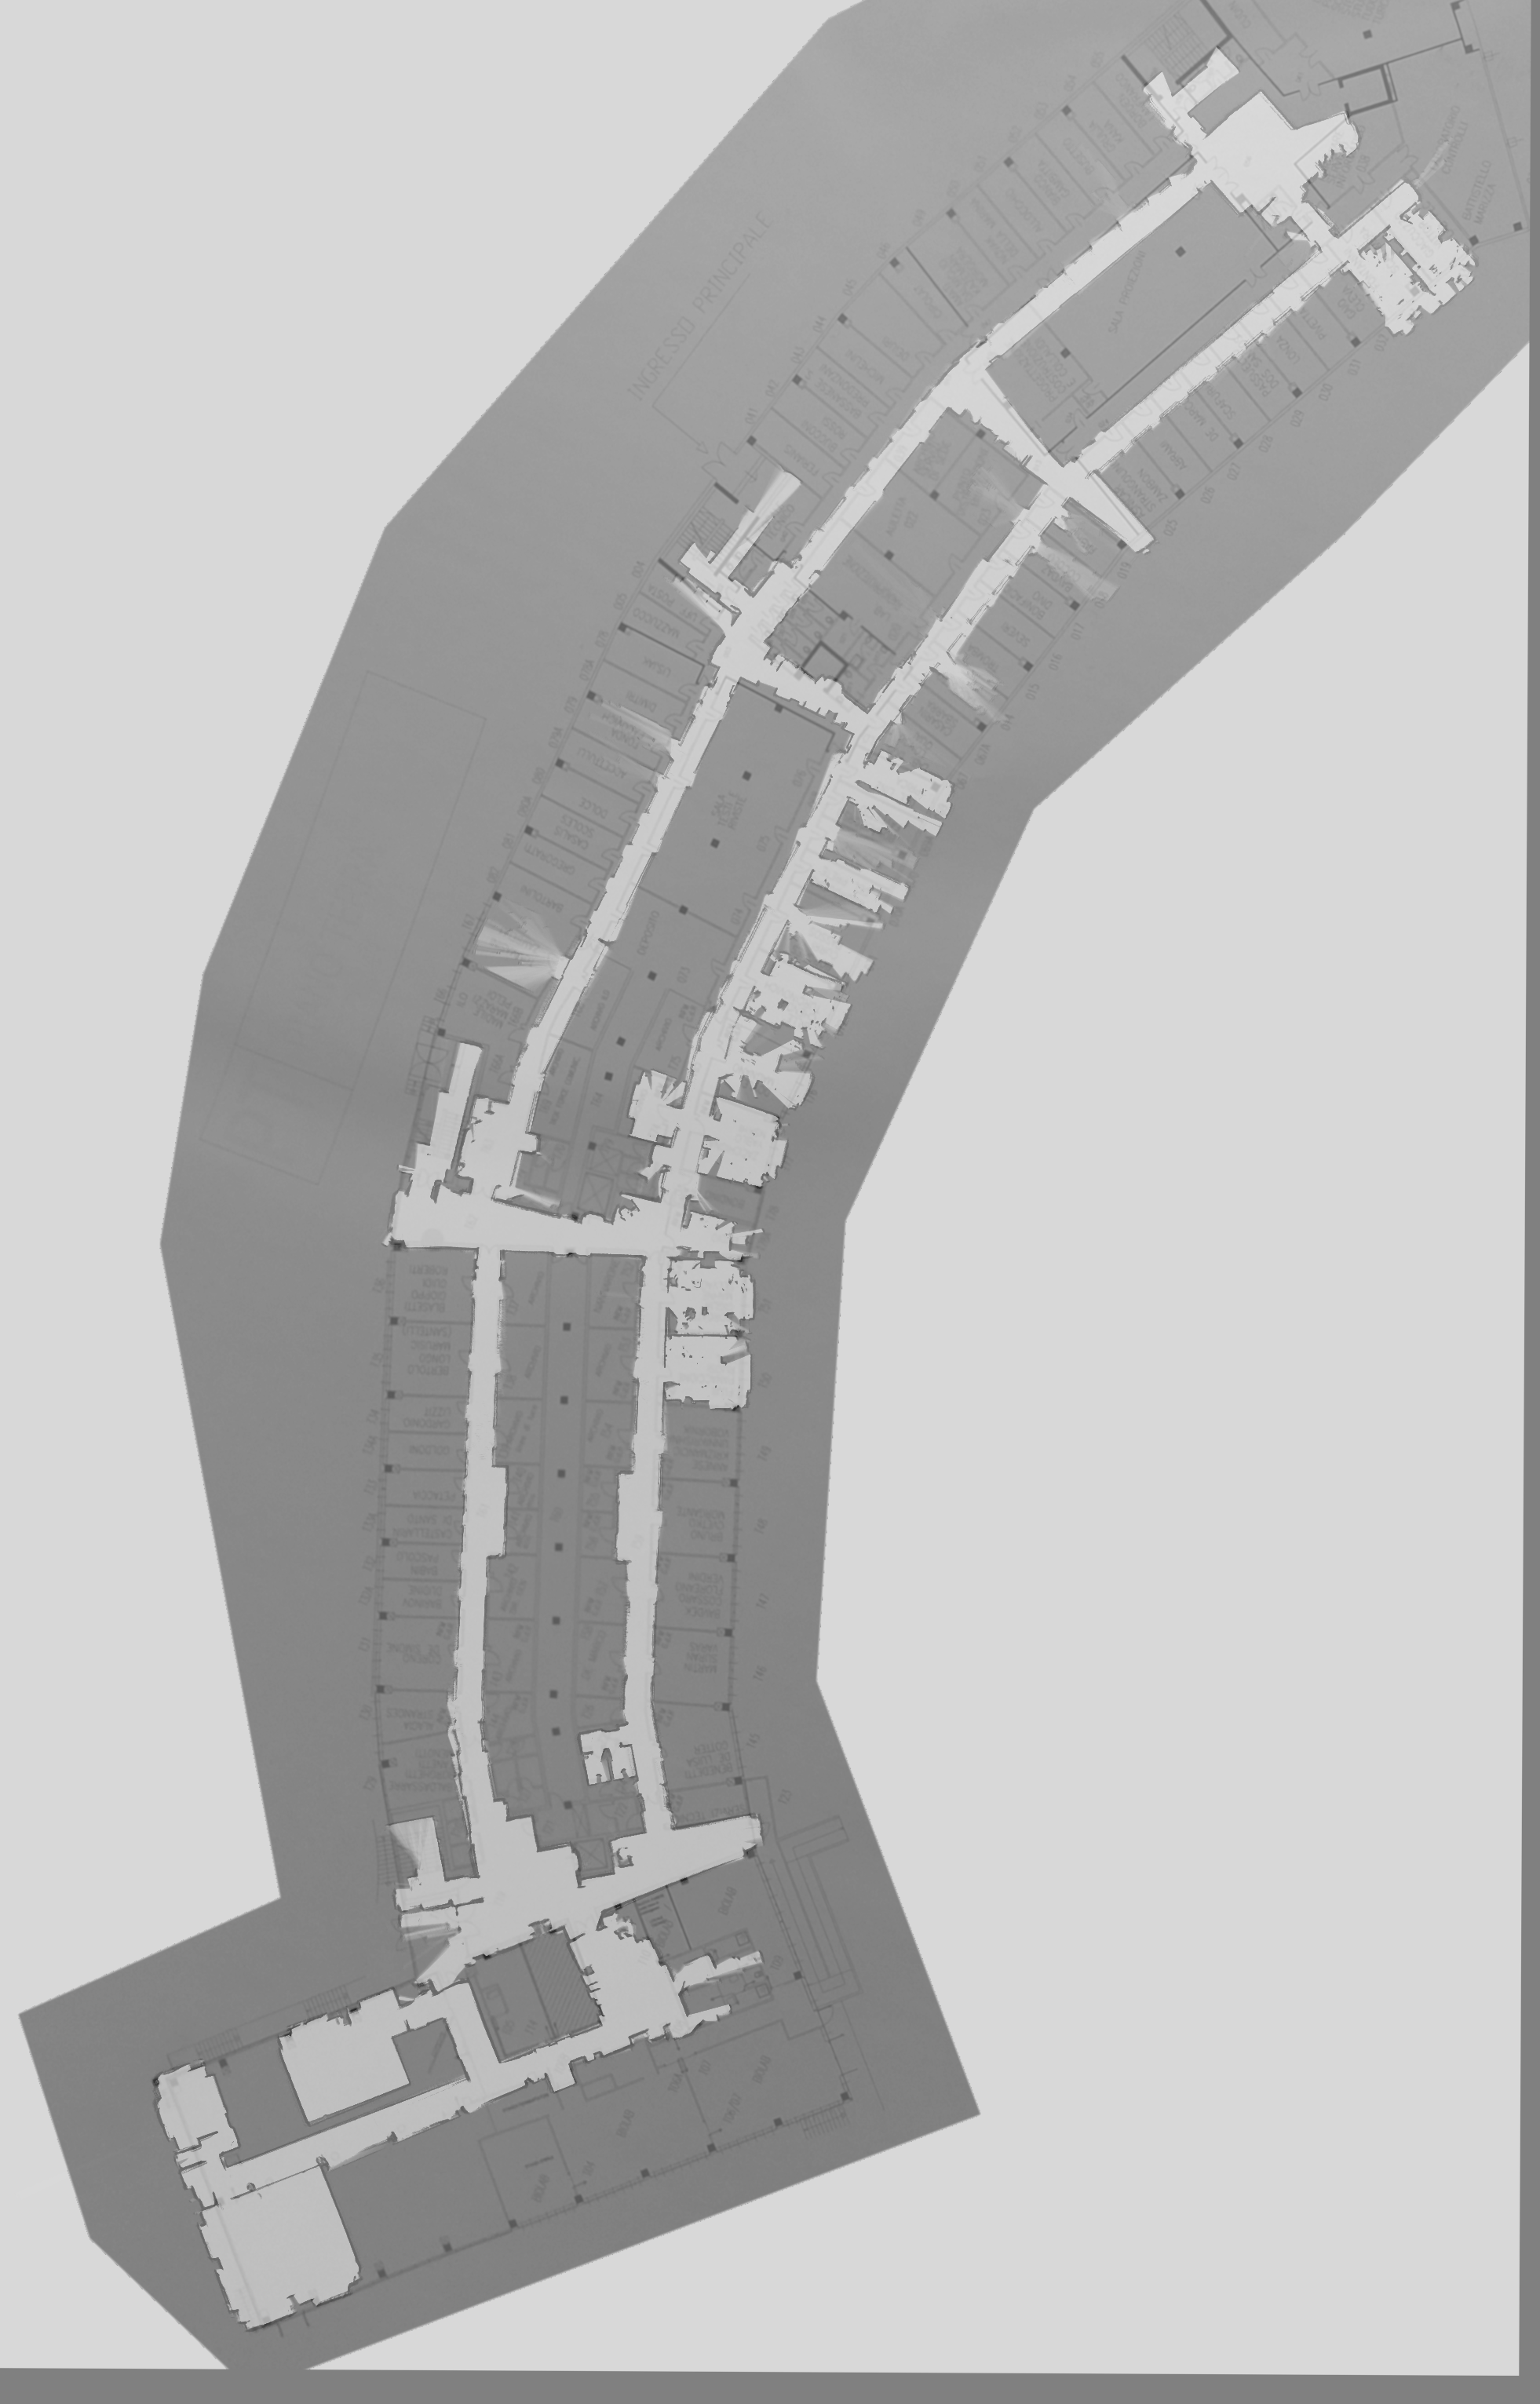
\includegraphics[width=0.7\linewidth]{img/mapComposizione.png}
	\captionof{figure}{Overlap Cartographer Map and photo of floor plan}
\end{figure}

\item For feaster the deployment of the robots, we used the  functionality of rosbag, a tool that allow to record the data published by some or all nodes and then republished after also with fastest velocity. This allot us to configure obtain the best outcome of process noise covariance of the localization node and the


\end{itemize}


\part{Results and Analysis}

\chapter{Presentation of results from testing and evaluation}
This part is divided based on the differents thing that have been completed:
\begin{itemize}
	\item porting the planner DStarGlobalPlanner from ROS 1 to ROS 2.
	\item given the robot platform rover mini build an autonomous mobile robot (AMR).
	\item given an the AMR jobot based on ROS 1 port it to ROS 2.
	\item implement the Open-RMF middleware using these robots.
\end{itemize}
\section{Porting the planner}
We have successfully port the code to ROS 2 and used for navigation. These are some output plan generated by the planner with different configuration parameters. More info about of the funtionality of the pramaters are described in its paper.
\\
\begin{figure}[h]
	\centering
	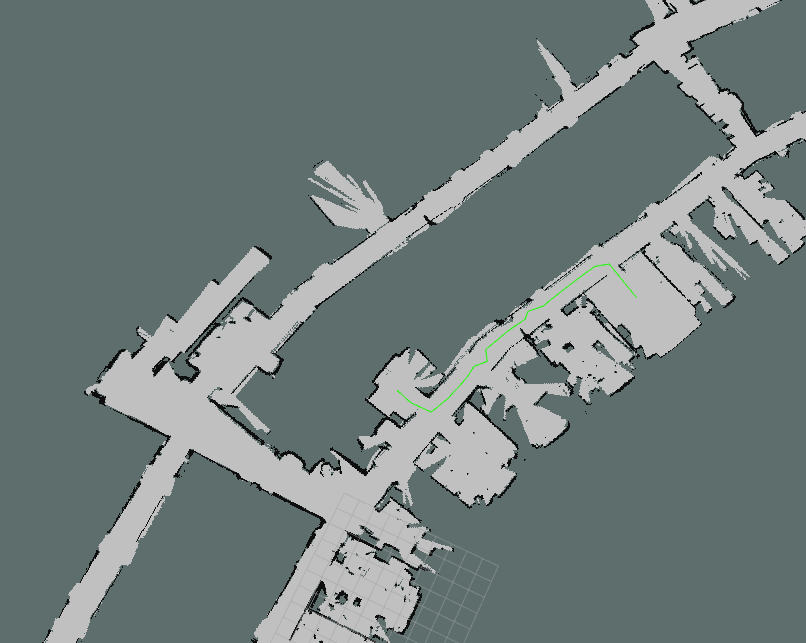
\includegraphics[width=0.6\linewidth]{img/Dstar_plan_ufficio_ripostiglio.png}
	\captionof{figure}{results obtained by the Dstar planner}
\end{figure}
\\
In the end, the logic transformation between the move\_base logic from ROS 1 to the Planner Server used in ROS 2 for the global planner are based on the implementation of the state machine Lyfecycle and the application of more advanced functionality of the languages used for programming.
\section{RoverRobotics Mini navigation result}
This are some images that display the Mini during navigation:\\
\begin{figure}[h]
\centering
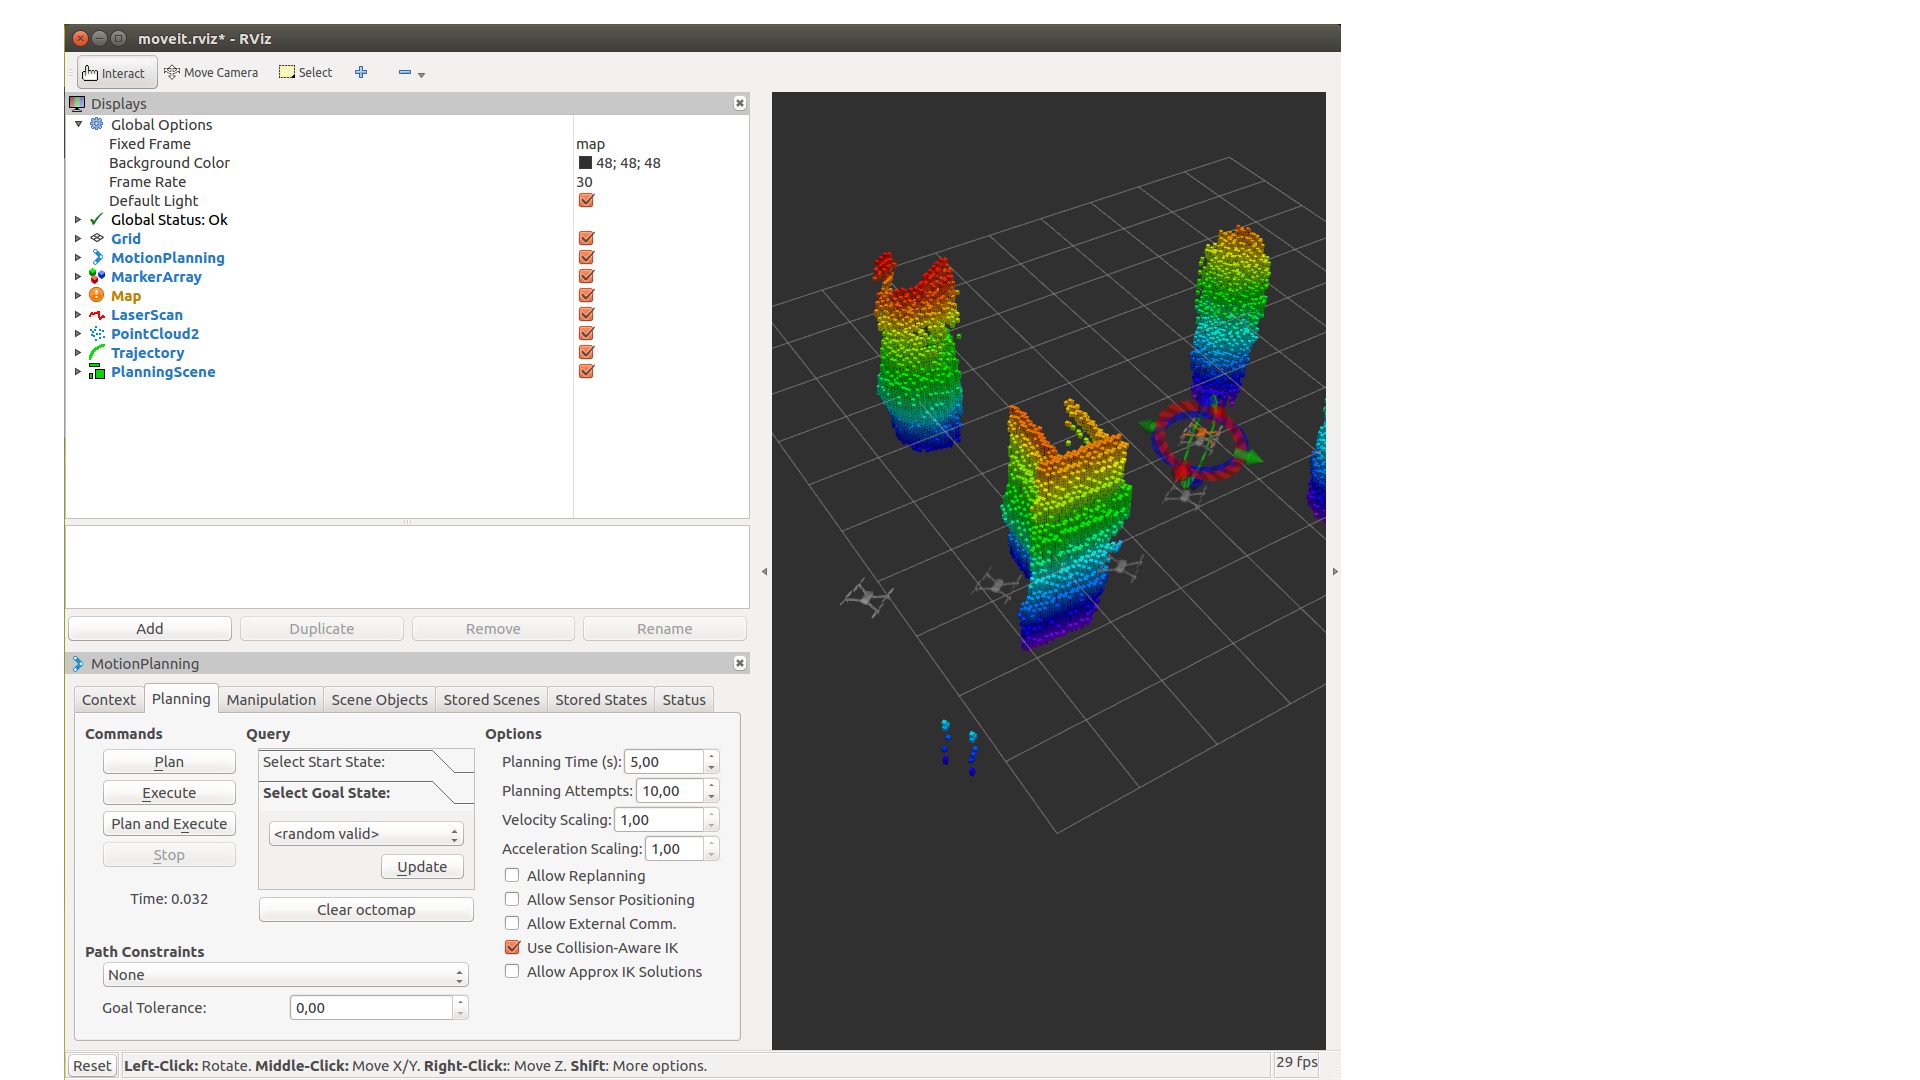
\includegraphics[width=0.7\linewidth]{img/rviz.png}
\captionof{figure}{results navigation of Mini}
\end{figure}
\\
The implementation was enough stray forward, building the robot and then apply the corrected nodes allow as to build a AMR. The tuning of the localization node and the localization node takes some time but is was reduced with the use of rosbag. 
\section{Jobot navigation result}
This are some images that display the Jobot during navigation:\\
\begin{figure}[h]
\centering
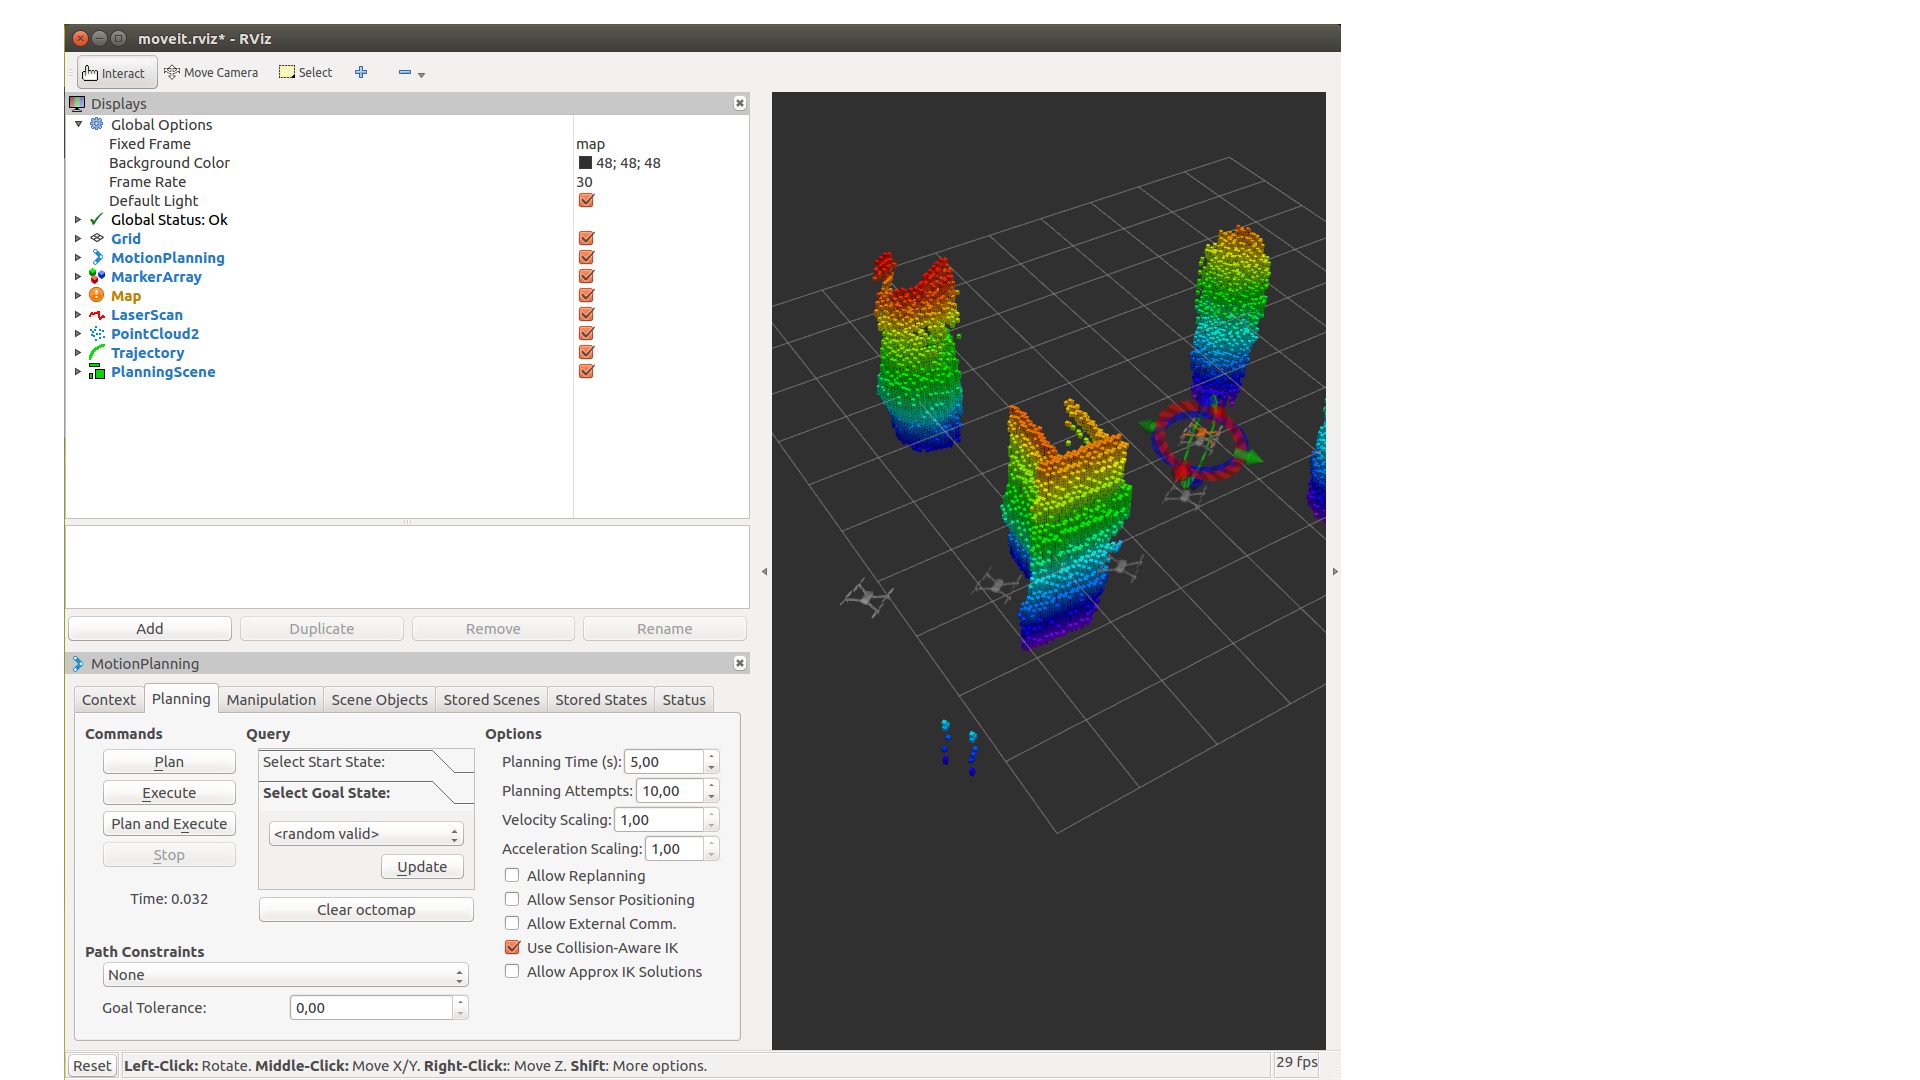
\includegraphics[width=0.7\linewidth]{img/rviz.png}
\captionof{figure}{results navigation of jobot}
\end{figure}
\\
Similar to the Mini, just more tuning.
\section{Open-RMF navigation result}
These are some images of the navigation of the 2 robots\\
\begin{figure}[h]
\centering
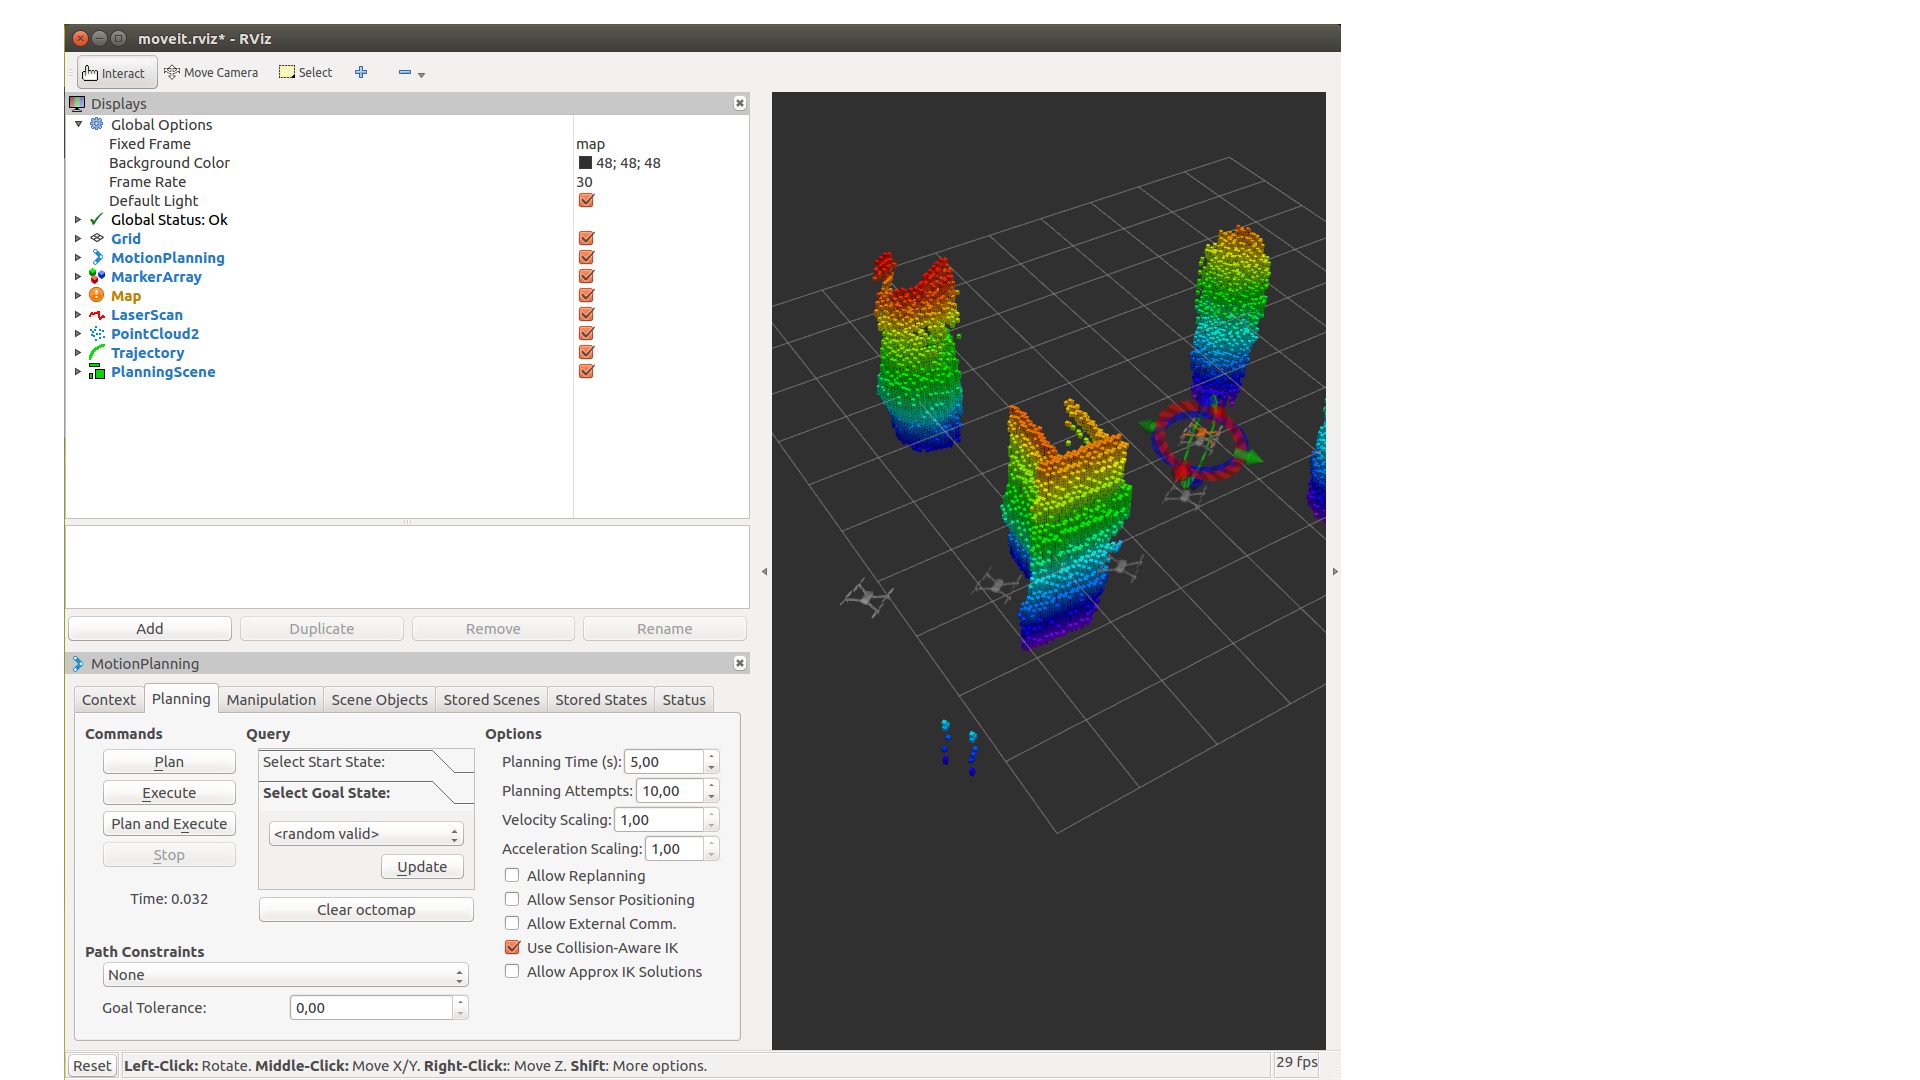
\includegraphics[width=0.7\linewidth]{img/rviz.png}
\captionof{figure}{images navigation of the 2 robots with open-rmf}
\end{figure}\\

\chapter{Comparison of system performance before and after the porting process}
This part is divided in section, in each section we evaluates the following:
\begin{itemize}
	\item calculation time for the planner on Mini rover
	\item navigation response from ROS 1 to ROS 2
\end{itemize}

\section{Planner calculation time comparisation before and after and vs new nav2 planner}
In this section, we present the time required for the global planner node to calculate the path from the planners, comparing the performance between the Jobot robot with ROS 1 built-in and the Docker ROS 2 image using the standard planner. \\
\begin{table}[h]
	\centering
	\begin{tabular}{|c|c|c|c|}
		\hline
		Start->End & ROS 1 D-start & ROS 2 D-start & ROS 2 NavfnPlanner \\
		\hline
		ufficio -> magazzino & 16.86 & 1.35 & 0.046 \\
		\hline
		ufficio -> ingresso & 73.238 & 1.35 & 0.073 \\
		\hline
		ingresso -> disegnatori & 60.41 & 1.35 & 0.081 \\
		\hline
	\end{tabular}
	\caption{result planner first request}
\end{table}\\
After the first iteration:
\begin{table}[h]
	\centering
	\begin{tabular}{|c|c|c|c|}
		\hline
		Start->End & ROS 1 D-start & ROS 2 D-start & ROS 2 NavfnPlanner \\
		\hline
		ufficio -> magazzino & 0.025 & 1.35 & 0.052 \\
		\hline
		ufficio -> ingresso & 0.091 & 1.35 & 0.069 \\
		\hline
		ingresso -> disegnatori & 0.158 & 1.35 & 0.084 \\
		\hline
	\end{tabular}
	\caption{result planner first request}
\end{table}\\

these are some results generated using the planner Dstar\\

\begin{figure}[h]
	\begin{subfigure}{.5\textwidth}
		\centering
		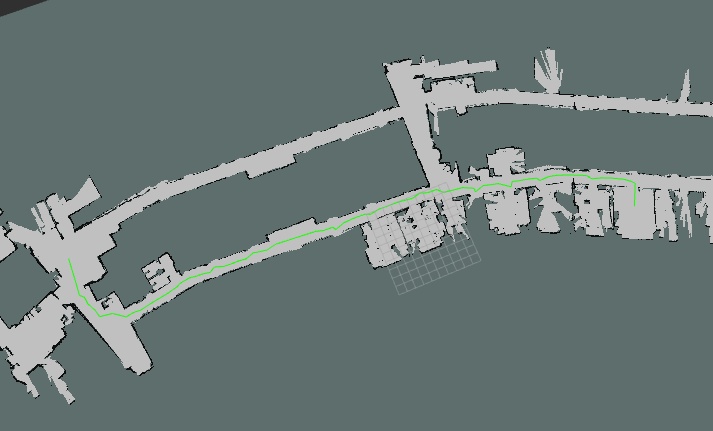
\includegraphics[width=.8\linewidth]{img/Dstar_plan_ufficio_ingresso.png}
	\end{subfigure}%
	\begin{subfigure}{.5\textwidth}
		\centering
		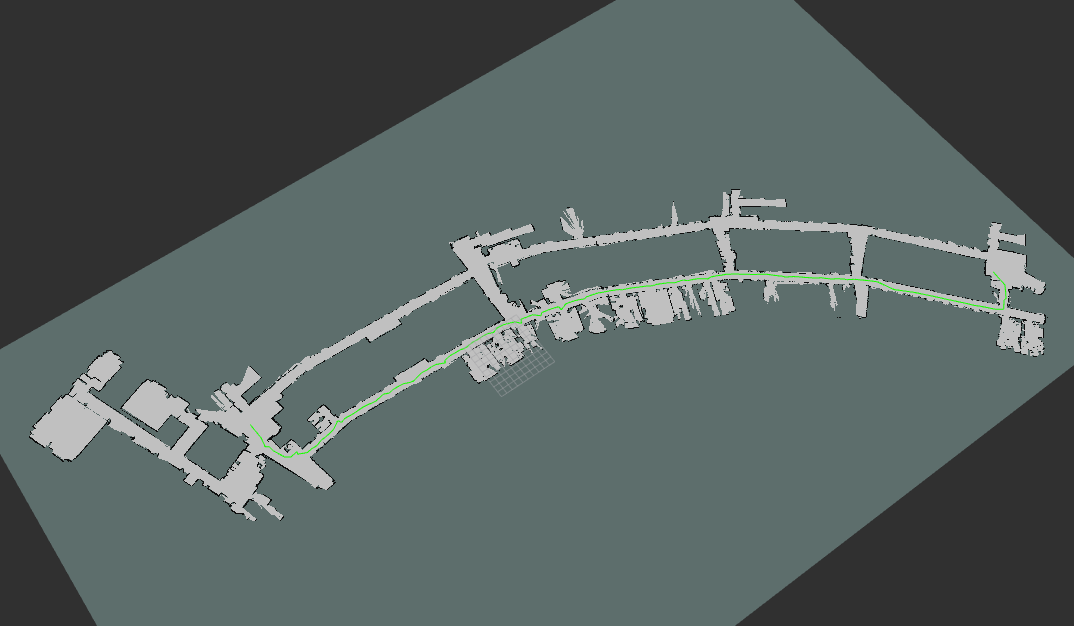
\includegraphics[width=.8\linewidth]{img/Dstar_plan_disegnatori_ingresso.png}
	\end{subfigure}
	\captionof{figure}{some of the plan generated by Dstar planner}
\end{figure}

and these are some generated by the NavfnPlanner

\begin{figure}[h]
	\begin{subfigure}{.5\textwidth}
		\centering
		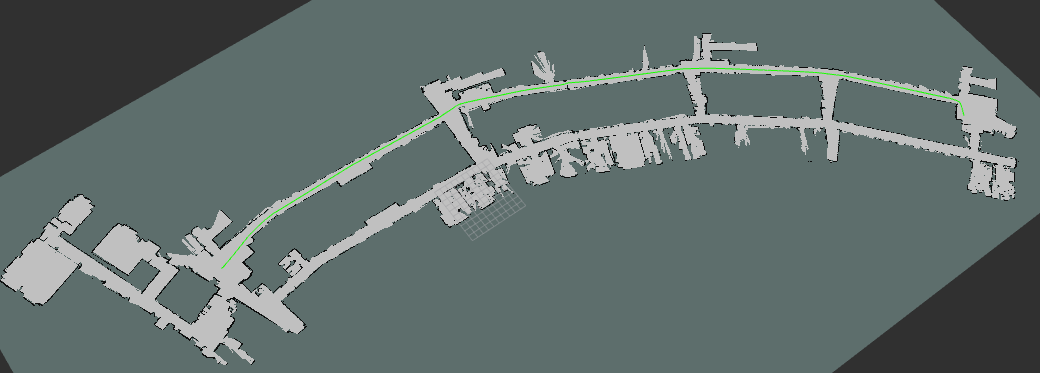
\includegraphics[width=.8\linewidth]{img/Navfn_plan_disegnatori_ingresso.png}
	\end{subfigure}%
	\begin{subfigure}{.5\textwidth}
		\centering
		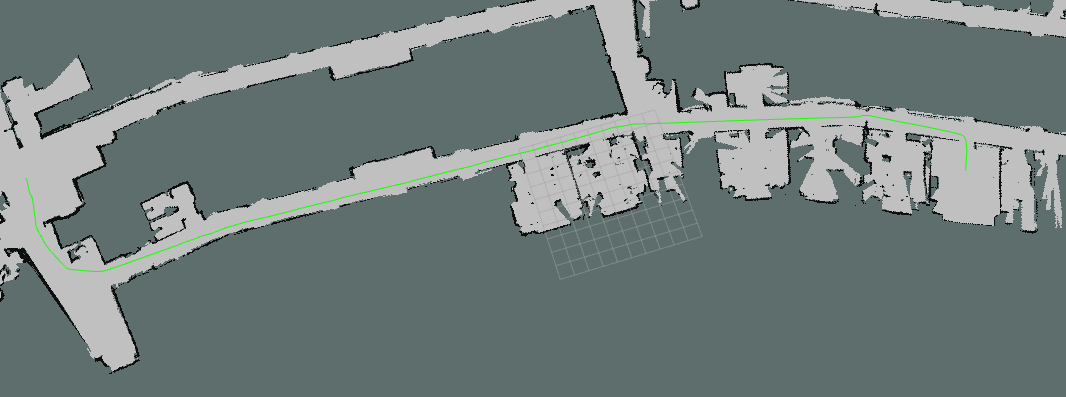
\includegraphics[width=.8\linewidth]{img/Navfn_plan_ufficio_ingresso.png}
	\end{subfigure}
	\captionof{figure}{some of the plan generated by NavfnPlanner planner}
\end{figure}

the result showed us:
\begin{itemize}
	\item time to calculate the first plan using Dstar is very higher than the NavfnPlanner
	\item after the first calculation the performances are similar
	\item without a fine tuning of the parameters of the Dstar planner hasnt returned an sub-optimal path
\end{itemize}

while porting there are some advantages that suggested an sub optimal application for open-rmf. it has an implemented a load from a file of paths but these need to reverse ingegneer to wrote down a json file compatible with that. A solution is to implement in the code a saving option for the planner.
 

\section{comparisation jobot navigation}
the test are performed using the same points as used before
\begin{table}[h]
	\centering
	\begin{tabular}{|c|c|c|}
		\hline
		Start->End & ROS 1 D-start & ROS 2 D-start \\
		\hline
		ufficio -> magazzino & 1.25 & 1.35\\
		\hline
		ufficio -> pausa lontana 1 & 1.25 & 1.35\\
		\hline
		magazzino -> pausa lontana 2 & 1.25 & 1.35\\
		\hline
	\end{tabular}
	\caption{result planner asking the node}
\end{table}
we obtain the following conclusion

\section{result analysis from Open-RMF}

\chapter{Discussion on the challenges encountered and how they were addressed}
the chalenges are:
\begin{itemize}
	\item high error on localization moving forward, it over estimate the movement comparing the map
	\item communication throught the wifi, since that the 
\end{itemize}




\part{Conclusion and Future Work}
Over this work we conclude the lot of benefits that the use of ROS 2 has made for an industrial standard.
\chapter{conclusion}
advantages using ROS 2 and his middleware structure (Zenoh)
\chapter{Future work}
improvement in the planner
\part{Appendices}
\chapter{Simulation}
In this part i will write some useful information for running the simulation.
All test were done on debian based machine:
To see the graphical interface launched in the docker container you need to have to share the access to the X server using the command \texttt{xhost local:root}.


today the tool for converting the data are 
\href{https://www.ros.org/blog/noetic-eol/}{https://www.ros.org/blog/noetic-eol/}

implement also \href{https://github.com/ros-navigation/navigation2/tree/main/tools/planner\_benchmarking}{planning benchmark}

describe and \textcolor{red}{use} composition in nav2 to obtain better performance \cite{10132508}


%\addcontentsline{toc}{chapter}{Bibliography}
%\bibliography{cap/references.bib}
\printbibliography
\end{document}